\documentclass[11pt,a4paper]{article}

% ── Packages ──────────────────────────────────────────────────────────
\usepackage[margin=0.85in,top=1in,bottom=1in]{geometry}
\usepackage{graphicx}
\usepackage{booktabs}
\usepackage{multirow}
\usepackage{amsmath,amssymb}
\usepackage{hyperref}
\usepackage{xcolor}
\usepackage{enumitem}
\usepackage{float}
\usepackage{caption}
\usepackage{subcaption}
\usepackage[numbers]{natbib}
\usepackage{fancyhdr}
\usepackage{titlesec}
\usepackage{parskip}
\usepackage{array}
\usepackage{makecell}
\usepackage{longtable}
\usepackage{colortbl}
\usepackage{adjustbox}
\usepackage{tikz}
\usepackage{multicol}
\usepackage{tabularx}
\usepackage{soul}
\usetikzlibrary{shapes.geometric,arrows,positioning,fit,calc,decorations.pathreplacing,backgrounds}

% ── Colors ────────────────────────────────────────────────────────────
\definecolor{bestblue}{RGB}{0,102,204}
\definecolor{lightgray}{gray}{0.95}
\definecolor{tabhead}{RGB}{41,65,122}
\definecolor{nodeblue}{RGB}{173,216,230}
\definecolor{nodegreen}{RGB}{144,238,144}
\definecolor{nodeorange}{RGB}{255,218,185}
\definecolor{nodepurple}{RGB}{216,191,216}
\definecolor{nodeyellow}{RGB}{255,255,153}
\definecolor{darkblue}{RGB}{0,0,139}
\definecolor{darkgreen}{RGB}{0,100,0}

% ── Page style ────────────────────────────────────────────────────────
\pagestyle{fancy}
\fancyhf{}
\rhead{\small ICD-10 Code Prediction from MIMIC-IV}
\lhead{\small NLP Final Project, Spring 2026}
\cfoot{\thepage}
\renewcommand{\headrulewidth}{0.4pt}

% ── Section formatting ────────────────────────────────────────────────
\titleformat{\section}{\Large\bfseries}{\thesection}{1em}{}[\vspace{2pt}\titlerule]
\titleformat{\subsection}{\large\bfseries}{\thesubsection}{1em}{}
\titleformat{\subsubsection}{\normalsize\bfseries}{\thesubsubsection}{1em}{}

% ── Hyperlink styling ─────────────────────────────────────────────────
\hypersetup{
    colorlinks=true,
    linkcolor=blue!70!black,
    citecolor=blue!70!black,
    urlcolor=blue!70!black,
}

% ── TikZ styles ───────────────────────────────────────────────────────
\tikzstyle{block} = [rectangle, rounded corners=4pt, minimum width=2.2cm,
    minimum height=0.7cm, text centered, text width=2.2cm, draw=black,
    font=\scriptsize\bfseries, line width=0.8pt]
\tikzstyle{arrow} = [thick,->,>=stealth]
\tikzstyle{dashed_box} = [rectangle, dashed, draw=gray!70, rounded corners=3pt,
    inner sep=4pt, line width=0.8pt]

\raggedbottom
\begin{document}

% ══════════════════════════════════════════════════════════════════════
% TITLE
% ══════════════════════════════════════════════════════════════════════
\begin{center}
    \vspace*{6pt}
    {\LARGE\bfseries ICD-10 Code Prediction from MIMIC-IV\\[4pt] Discharge Summaries}\\[16pt]
    {\large\textbf{Rohan Kumar Chitra} \quad\quad \textbf{Deva Sai Sunder Tangella}}\\[6pt]
    {\normalsize NLP Final Project, Spring 2026}
\end{center}

\vspace{6pt}
\noindent\rule{\textwidth}{1.0pt}

% ── Contributions ─────────────────────────────────────────────────────
\subsection*{Individual Contributions}

\begin{minipage}[t]{0.48\textwidth}
\textbf{Rohan Kumar Chitra} \textit{(Approach 1: Chunk-BERT + Label Attention)}
\begin{itemize}[nosep,leftmargin=1.2em]
    \item Designed sliding-window chunking (6$\times$512 tokens, stride 256) for full-document coverage.
    \item Implemented per-label attention with 50 learnable query vectors over Bio\_ClinicalBERT.
    \item Two-phase training: frozen encoder $\rightarrow$ fine-tune last 2 BERT layers.
    \item MIMIC-IV data extraction pipeline and cohort construction (122,304 admissions).
    \item Text preprocessing: de-identification stripping, normalization, TF-IDF engineering.
    \item Shared evaluation framework (threshold tuning, head/torso/tail analysis).
\end{itemize}
\end{minipage}
\hfill
\begin{minipage}[t]{0.48\textwidth}
\textbf{Deva Sai Sunder Tangella} \textit{(Approach 2: BiLSTM-LAAT)}
\begin{itemize}[nosep,leftmargin=1.2em]
    \item Implemented LAAT architecture: BiLSTM encoder + structured label attention.
    \item Word-level tokenization with 50,000-word vocabulary, native 4,000-token processing.
    \item Temperature calibration post-training (ECE: 0.07 $\rightarrow$ 0.02).
    \item Comparative evaluation: scatter analysis, bar charts, confusion matrices.
    \item Production packaging: \texttt{src/} module, FastAPI REST API, Streamlit demo.
    \item Pytest test suite: data processing, model shapes, API schema validation.
\end{itemize}
\end{minipage}

\smallskip
\noindent\textbf{Shared:} TF-IDF + SGD baseline, Bio\_ClinicalBERT truncation baseline, ensemble experiments, Streamlit web demo, report writing.

\vspace{6pt}
\noindent\rule{\textwidth}{1.0pt}
\vspace{6pt}

% ══════════════════════════════════════════════════════════════════════
% ABSTRACT
% ══════════════════════════════════════════════════════════════════════
\begin{abstract}
\noindent Manual assignment of ICD-10 diagnosis codes costs the U.S.\ healthcare system roughly \$25 billion a year, and the process is slow, tedious, and error prone. We frame ICD-10 coding as a multi-label classification task over the 50 most frequent codes in MIMIC-IV, covering 122,304 hospital admissions. Starting from a TF-IDF + SGD baseline (Micro F1 of 0.60), we develop two neural architectures that can handle full length discharge summaries: a Chunk-BERT architecture with per-label attention that processes full documents via overlapping 512-token windows over Bio\_ClinicalBERT, and a BiLSTM with Label-Aware Attention (BiLSTM-LAAT) encoding up to 4,000 word tokens in a single pass. BiLSTM-LAAT turns out to be the strongest single model, reaching Micro F1 of 0.72 with balanced precision and recall. A weighted ensemble combining BiLSTM-LAAT and TF-IDF + SGD maintains Micro F1 at 0.72 while pushing Macro F1 to 0.67 and AUROC to 0.95. Error analysis reveals that clinically related code pairs (e.g., systolic vs.\ diastolic heart failure) and administrative codes (e.g., BMI categories, DNR status) remain the most challenging. We provide a complete system including a Streamlit web demo and FastAPI service.
\end{abstract}

% ══════════════════════════════════════════════════════════════════════
% 1. INTRODUCTION
% ══════════════════════════════════════════════════════════════════════
\section{Introduction}

\subsection{Motivation}
Every hospital encounter in the United States gets tagged with a set of ICD-10 codes that drive billing, epidemiological tracking, and quality reporting. In practice, trained clinical coders read through discharge summaries and assign these codes by hand, a process that costs the healthcare system an estimated \$25 billion annually \cite{mullenbach2018explainable}. It is also slow and inconsistent: coders disagree on edge cases, and backlogs delay reimbursement. Automating even part of this workflow would save money, catch errors earlier, and speed up the revenue cycle.

\subsection{Problem Definition}
Given a clinical discharge summary $\mathbf{x}$ (typically 800--2,000 words), predict the set of ICD-10 diagnosis codes $\mathbf{y} = \{y_1, y_2, \ldots, y_k\}$ assigned to the hospital encounter. This is a \textit{multi-label classification} problem over the top-50 most frequent ICD-10 codes in MIMIC-IV.

\subsection{Challenges}
Several factors make this problem difficult. First, the label space is enormous: after filtering codes that appear fewer than 10 times we still have 7,940 unique ICD-10 codes, and the distribution is heavily long-tailed, with rare codes showing up in fewer than 0.10\% of admissions. Second, discharge summaries are long. The average note runs about 1,500 words (Figure \ref{fig:note_length}), well beyond BERT's 512-token window, so any transformer-based approach has to deal with truncation or chunking. Third, clinical language is messy: the same diagnosis can be phrased in many different ways, peppered with abbreviations and negation. Finally, ICD codes do not appear in isolation. Hypertension commonly co-occurs with diabetes, and closely related subtypes like systolic versus diastolic heart failure regularly trip up classifiers.

\subsection{Contributions}
Our main contributions are as follows. We build an end-to-end ICD-10 prediction pipeline on MIMIC-IV for the top-50 codes, using patient-level splits to avoid data leakage. We propose and compare two neural architectures that process full-length notes: Chunk-BERT with per-label attention and BiLSTM-LAAT. Across five individual models and five ensemble configurations we carry out a detailed error analysis, including per-label confusion matrices, head-versus-tail breakdowns, and identification of the most confused code pairs. We also package the best model into a Streamlit web interface backed by a FastAPI service.

% ── System Overview Diagram ────────────────────────────────────────────
\begin{figure}[H]
\centering
\resizebox{0.98\textwidth}{!}{%
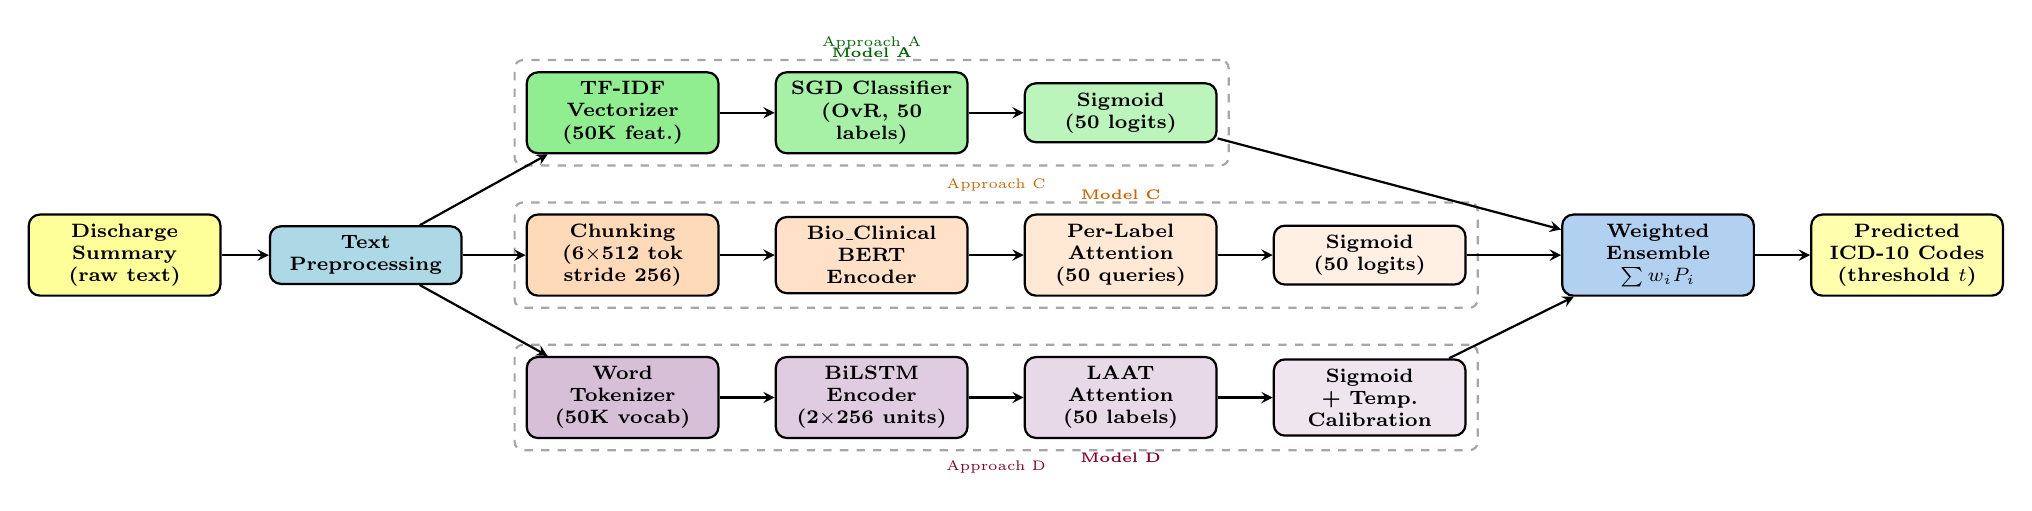
\begin{tikzpicture}[node distance=0.55cm and 0.45cm]

% ── Input ────
\node[block, fill=nodeyellow] (input) {Discharge Summary\\(raw text)};

% ── Preprocessing ────
\node[block, fill=nodeblue, right=0.6cm of input] (preprocess) {Text\\Preprocessing};

% ── Three paths ────
\node[block, fill=nodegreen, above right=0.9cm and 0.8cm of preprocess] (tfidf) {TF-IDF\\Vectorizer\\(50K feat.)};
\node[block, fill=nodeorange, right=0.8cm of preprocess] (chunk) {Chunking\\(6$\times$512 tok\\stride 256)};
\node[block, fill=nodepurple, below right=0.9cm and 0.8cm of preprocess] (bilstm_tok) {Word\\Tokenizer\\(50K vocab)};

% ── Model encoders ────
\node[block, fill=nodegreen!80, right=0.7cm of tfidf] (sgd) {SGD Classifier\\(OvR, 50 labels)};
\node[block, fill=nodeorange!80, right=0.7cm of chunk] (bert) {Bio\_Clinical\\BERT\\Encoder};
\node[block, fill=nodepurple!80, right=0.7cm of bilstm_tok] (bilstm) {BiLSTM\\Encoder\\(2$\times$256 units)};

% ── Attention / head ────
\node[block, fill=nodeorange!60, right=0.7cm of bert] (lbl_attn) {Per-Label\\Attention\\(50 queries)};
\node[block, fill=nodepurple!60, right=0.7cm of bilstm] (laat) {LAAT\\Attention\\(50 labels)};

% ── Classifiers ────
\node[block, fill=nodegreen!60, right=0.7cm of sgd] (sigA) {Sigmoid\\(50 logits)};
\node[block, fill=nodeorange!40, right=0.7cm of lbl_attn] (sigC) {Sigmoid\\(50 logits)};
\node[block, fill=nodepurple!40, right=0.7cm of laat] (sigD) {Sigmoid + Temp.\\Calibration};

% ── Ensemble ────
\node[block, fill=bestblue!30, right=1.2cm of sigC] (ensemble) {Weighted\\Ensemble\\$\sum w_i P_i$};

% ── Output ────
\node[block, fill=nodeyellow!80, right=0.7cm of ensemble] (output) {Predicted\\ICD-10 Codes\\(threshold $t$)};

% ── Arrows ────
\draw[arrow] (input) -- (preprocess);
\draw[arrow] (preprocess) -- (tfidf);
\draw[arrow] (preprocess) -- (chunk);
\draw[arrow] (preprocess) -- (bilstm_tok);
\draw[arrow] (tfidf) -- (sgd);
\draw[arrow] (chunk) -- (bert);
\draw[arrow] (bilstm_tok) -- (bilstm);
\draw[arrow] (sgd) -- (sigA);
\draw[arrow] (bert) -- (lbl_attn);
\draw[arrow] (bilstm) -- (laat);
\draw[arrow] (lbl_attn) -- (sigC);
\draw[arrow] (laat) -- (sigD);
\draw[arrow] (sigA) -- (ensemble);
\draw[arrow] (sigC) -- (ensemble);
\draw[arrow] (sigD) -- (ensemble);
\draw[arrow] (ensemble) -- (output);

% ── Model labels ────
\node[above=0.05cm of sgd, font=\tiny\bfseries\color{darkgreen}] {Model A};
\node[above=0.05cm of lbl_attn, font=\tiny\bfseries\color{orange!80!black}] {Model C};
\node[below=0.05cm of laat, font=\tiny\bfseries\color{purple!70!black}] {Model D};

% ── Dashed boxes ────
\begin{scope}[on background layer]
\node[dashed_box, fit=(tfidf)(sgd)(sigA), label={[font=\tiny,color=darkgreen]above:Approach A}] {};
\node[dashed_box, fit=(chunk)(bert)(lbl_attn)(sigC), label={[font=\tiny,color=orange!80!black]above:Approach C}] {};
\node[dashed_box, fit=(bilstm_tok)(bilstm)(laat)(sigD), label={[font=\tiny,color=purple!70!black]below:Approach D}] {};
\end{scope}

\end{tikzpicture}
}
\caption{Overall system architecture. Three model families process discharge summaries independently; their sigmoid probabilities are combined via weighted ensemble, and a global threshold produces final ICD-10 predictions.}
\label{fig:system}
\end{figure}

% ══════════════════════════════════════════════════════════════════════
% 2. PRIOR WORK
% ══════════════════════════════════════════════════════════════════════
\section{Prior Work}

Research on automated ICD coding has moved through several phases. Early systems relied on bag-of-words features with SVMs or logistic regression applied to MIMIC-III notes \cite{perotte2014diagnosis}, and TF-IDF baselines with one-vs-rest classifiers still hold up surprisingly well because ICD codes often hinge on specific medical terms.

\citet{mullenbach2018explainable} introduced CAML, a CNN encoder paired with per-label attention, along with a description-regularized variant (DR-CAML) that used ICD code descriptions as auxiliary supervision. This work established per-label attention as a key ingredient for multi-label clinical coding.

More recently, \citet{huang2022plmicd} showed that combining a pretrained language model with overlapping text chunks and per-label attention (PLM-ICD) could reach state-of-the-art on MIMIC-III across the full label set. Our Chunk-BERT architecture borrows heavily from this design. On the recurrent side, \citet{vu2020label} proposed LAAT, a BiLSTM with structured label attention that matched or beat transformer-based methods at a fraction of the training cost. We adopt this idea in our BiLSTM-LAAT model.

For the encoder, we use Bio\_ClinicalBERT \cite{alsentzer2019publicly}, which was pretrained on MIMIC-III clinical notes. Its 512-token limit throws away a large portion of each discharge summary, which is exactly why we need the chunking and recurrent strategies described above. To handle class imbalance, we use focal loss \cite{lin2017focal} in both Chunk-BERT v2 and BiLSTM-LAAT, down-weighting easy examples so the model pays more attention to rare codes.

% ══════════════════════════════════════════════════════════════════════
% 3. DATASET
% ══════════════════════════════════════════════════════════════════════
\section{Dataset}

\subsection{Data Source}
All experiments use MIMIC-IV \cite{johnson2023mimiciv}, a de-identified collection of electronic health records from Beth Israel Deaconess Medical Center. We pull data from two tables: \texttt{discharge}, which contains 331,793 clinical notes, and \texttt{diagnoses\_icd}, with 6,364,488 code assignments. Joining these on admission identifiers and dropping rows that lack either a note or an ICD-10 code leaves us with \textbf{122,304 admissions}.

\subsection{Label Statistics and Data Split}

\begin{table}[H]
\centering
\caption{Dataset statistics overview.}
\label{tab:data_stats}
\small
\begin{tabular}{lrl}
\toprule
\textbf{Statistic} & \textbf{Value} & \textbf{Note} \\
\midrule
Total discharge notes                      & 331,793 & 100\% of notes \\
Admissions with notes + ICD-10 codes       & 122,304 & 36.86\% \\
Unique ICD-10 codes (freq $\geq$ 10)      & 7,940   & Full label space \\
Top-$K$ codes used in experiments          & 50      & 0.63\% of 7,940 \\
Top-50 label coverage (code assignments)   & 32.50\% & Benchmark standard \\
Mean labels per admission                  & 5.10    & Multi-label \\
Mean note length (words)                   & 1,500   & Exceeds 512-tok limit \\
\bottomrule
\end{tabular}
\end{table}

We split by patient (seed = 42) so that no patient's admissions appear in more than one partition:

\begin{table}[H]
\centering
\caption{Train / validation / test split sizes.}
\label{tab:split}
\small
\begin{tabular}{lcccc}
\toprule
\textbf{Split} & \textbf{Admissions} & \textbf{Percentage} & \textbf{Label matrix shape} \\
\midrule
Train      & 85,081  & 69.57\% & $(85{,}081 \times 50)$ \\
Validation & 18,371  & 15.02\% & $(18{,}371 \times 50)$ \\
Test       & 18,852  & 15.41\% & $(18{,}852 \times 50)$ \\
\midrule
\textbf{Total} & \textbf{122,304} & \textbf{100\%} & -- \\
\bottomrule
\end{tabular}
\end{table}

\subsection{Preprocessing}
We clean each note by stripping out the de-identification placeholders (\texttt{[** ... **]}), lowercasing, removing non-alphanumeric characters (while keeping medical values like ``WBC-4.80''), and collapsing extra whitespace. For the ClinicalBERT baseline, which is limited to 512 tokens, we apply a \emph{smart truncation} heuristic that uses regex patterns to keep the discharge diagnoses, hospital course, and history of present illness sections, since those tend to carry the most coding-relevant information.

\begin{figure}[H]
\centering
\begin{subfigure}[b]{0.48\textwidth}
\centering
\resizebox{\textwidth}{!}{%
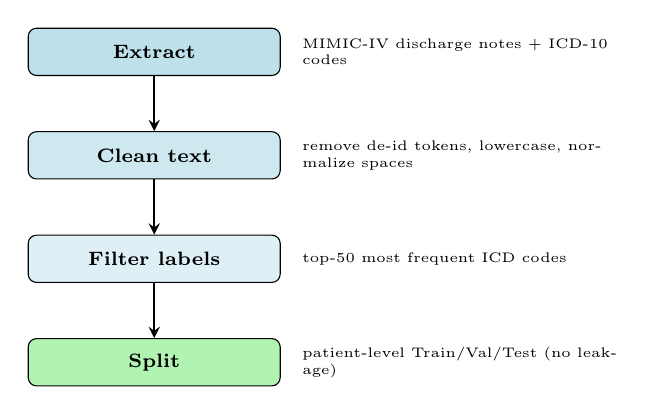
\begin{tikzpicture}[
    step/.style={rectangle, rounded corners=3pt, draw=black, fill=#1,
                 minimum width=3.2cm, minimum height=0.6cm, text centered,
                 font=\scriptsize\bfseries, text=black},
    desc/.style={font=\tiny, anchor=west, text width=4cm},
    arrow/.style={->, thick, >=stealth},
    node distance=0.7cm
]
\node[step=nodeblue!80] (s1) {Extract};
\node[desc, right=0.15cm of s1] (d1) {MIMIC-IV discharge notes + ICD-10 codes};
\node[step=nodeblue!60, below=of s1] (s2) {Clean text};
\node[desc, right=0.15cm of s2] (d2) {remove de-id tokens, lowercase, normalize spaces};
\node[step=nodeblue!40, below=of s2] (s3) {Filter labels};
\node[desc, right=0.15cm of s3] (d3) {top-50 most frequent ICD codes};
\node[step=nodegreen!70, below=of s3] (s4) {Split};
\node[desc, right=0.15cm of s4] (d4) {patient-level Train/Val/Test (no leakage)};
\draw[arrow] (s1) -- (s2);
\draw[arrow] (s2) -- (s3);
\draw[arrow] (s3) -- (s4);
\end{tikzpicture}
}
\caption{Text preprocessing pipeline}
\end{subfigure}
\hfill
\begin{subfigure}[b]{0.48\textwidth}
\centering
\resizebox{\textwidth}{!}{%
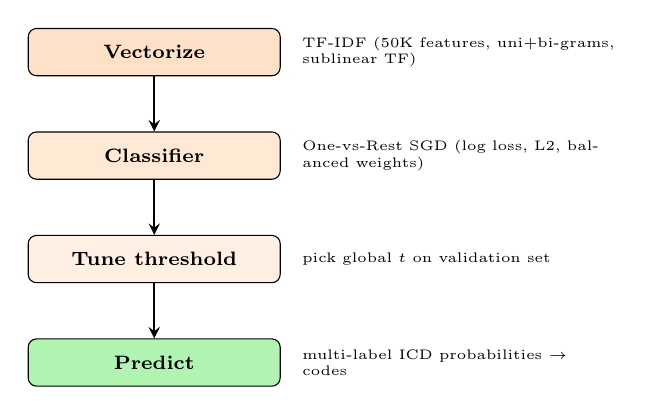
\begin{tikzpicture}[
    step/.style={rectangle, rounded corners=3pt, draw=black, fill=#1,
                 minimum width=3.2cm, minimum height=0.6cm, text centered,
                 font=\scriptsize\bfseries, text=black},
    desc/.style={font=\tiny, anchor=west, text width=4cm},
    arrow/.style={->, thick, >=stealth},
    node distance=0.7cm
]
\node[step=nodeorange!80] (s1) {Vectorize};
\node[desc, right=0.15cm of s1] (d1) {TF-IDF (50K features, uni+bi-grams, sublinear TF)};
\node[step=nodeorange!60, below=of s1] (s2) {Classifier};
\node[desc, right=0.15cm of s2] (d2) {One-vs-Rest SGD (log loss, L2, balanced weights)};
\node[step=nodeorange!40, below=of s2] (s3) {Tune threshold};
\node[desc, right=0.15cm of s3] (d3) {pick global $t$ on validation set};
\node[step=nodegreen!70, below=of s3] (s4) {Predict};
\node[desc, right=0.15cm of s4] (d4) {multi-label ICD probabilities $\rightarrow$ codes};
\draw[arrow] (s1) -- (s2);
\draw[arrow] (s2) -- (s3);
\draw[arrow] (s3) -- (s4);
\end{tikzpicture}
}
\caption{TF-IDF feature extraction pipeline}
\end{subfigure}
\caption{Data preprocessing and feature engineering pipelines.}
\label{fig:preprocessing}
\end{figure}

\subsection{Exploratory Data Analysis}

\begin{figure}[H]
    \centering
    \begin{subfigure}[b]{0.48\textwidth}
        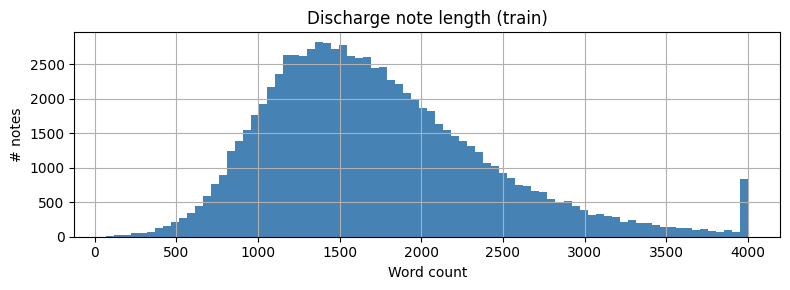
\includegraphics[width=\textwidth]{figures/note_length_dist.png}
        \caption{Distribution of discharge note lengths (words).}
        \label{fig:note_length}
    \end{subfigure}
    \hfill
    \begin{subfigure}[b]{0.48\textwidth}
        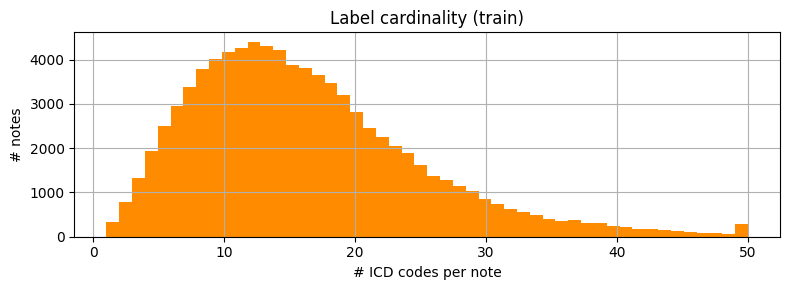
\includegraphics[width=\textwidth]{figures/label_cardinality.png}
        \caption{Distribution of label cardinality per admission.}
        \label{fig:label_card}
    \end{subfigure}
    \caption{Exploratory data analysis of MIMIC-IV discharge notes.}
\end{figure}

\begin{figure}[H]
    \centering
    \begin{subfigure}[b]{0.48\textwidth}
        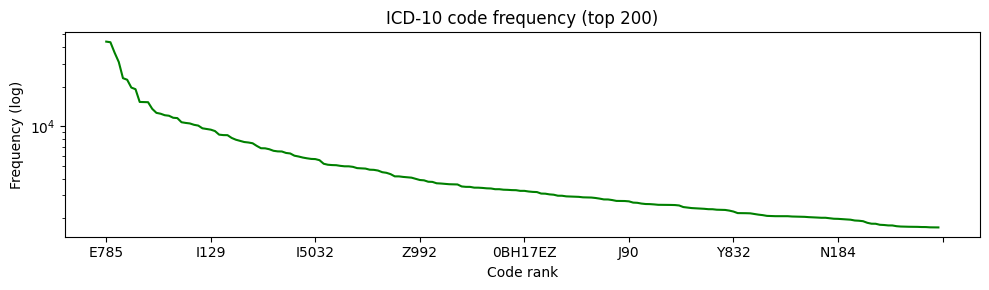
\includegraphics[width=\textwidth,height=5.5cm,keepaspectratio]{figures/code_freq_tail.png}
        \caption{Top-200 ICD-10 code frequencies (long-tail distribution).}
        \label{fig:code_freq}
    \end{subfigure}
    \hfill
    \begin{subfigure}[b]{0.48\textwidth}
        
\includegraphics[width=\textwidth,height=5.5cm,keepaspectratio]{figures/split_counts.png}
        \caption{Number of admissions and percentage per data split.}
        \label{fig:split_counts}
    \end{subfigure}
    \caption{Label distribution and data split visualization.}
\end{figure}

% ══════════════════════════════════════════════════════════════════════
% 4. METHODS
% ══════════════════════════════════════════════════════════════════════
\section{Methods}

We experiment with five models spanning three families: a TF-IDF + SGD baseline, a truncated ClinicalBERT baseline, Chunk-BERT with label attention, BiLSTM-LAAT, and several weighted-probability ensembles. Figure \ref{fig:system} shows how the pieces fit together.

\subsection{TF-IDF + SGD (Model A: Baseline)}

\textbf{Feature extraction.} TF-IDF vectorization with 50,000 features, unigram+bigram range, and sublinear TF scaling ($1 + \log(\text{tf})$) $\rightarrow$ sparse matrix $\mathbf{X} \in \mathbb{R}^{n \times 50{,}000}$.

\textbf{Classifier.} \texttt{OneVsRestClassifier} wrapping \texttt{SGDClassifier} with log-loss, L2 regularization, and balanced class weights. Global threshold sweep on validation set $\rightarrow$ $t^* = 0.53$.

\textbf{Training time:} roughly 2 minutes on CPU, compared to hours when training on the full 7,940-label set with SAGA.

\subsection{ClinicalBERT with Truncation (Model B: Baseline)}

This baseline fine-tunes Bio\_ClinicalBERT \cite{alsentzer2019publicly}, taking the \texttt{[CLS]} embedding through dropout ($p = 0.10$) and a 50-output linear head. Smart truncation keeps the most informative sections within the 512-token window. We train for 3 epochs with AdamW ($\text{lr} = 2\times10^{-5}$), BCE loss, and fp16 mixed precision. The best threshold on the validation set is $t^* = 0.28$. Training loss drops from 0.29 to 0.22, and validation Micro-F1 reaches 0.47.

Even with smart truncation, 512 tokens is not enough. The average note is about 1,500 words, so ClinicalBERT throws away the majority of the document. The next two approaches tackle this limitation head-on.

\subsection{Approach 1: Chunk-BERT + Label Attention (Model C)}
\label{sec:chunk_bert}

Our first proposed approach follows the PLM-ICD recipe \cite{huang2022plmicd}: split the document into overlapping 512-token windows, encode each with Bio\_ClinicalBERT, and let a per-label attention layer pick out the relevant pieces.

\begin{figure}[H]
\centering
\resizebox{0.92\textwidth}{!}{%
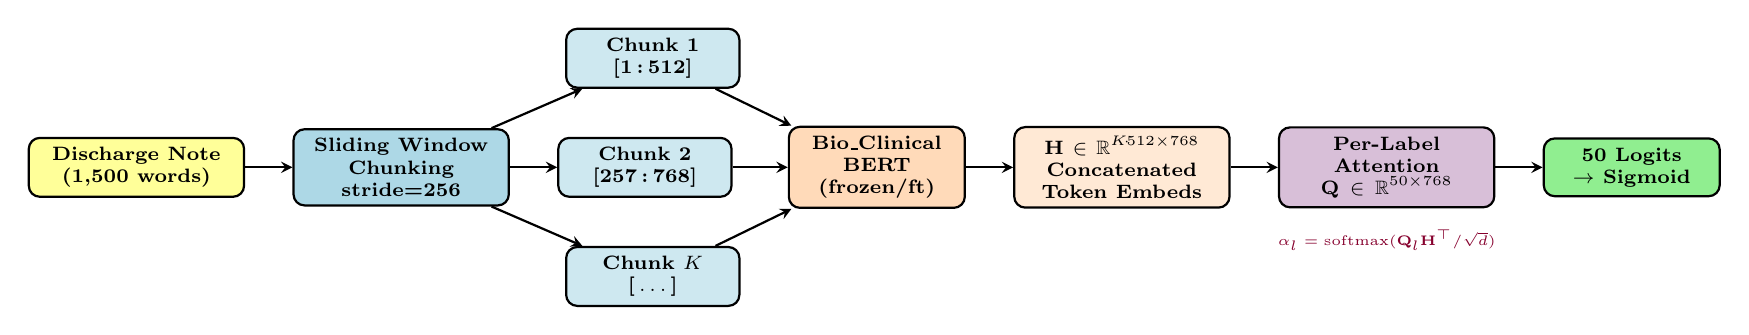
\begin{tikzpicture}[node distance=0.5cm and 0.5cm]
% Input
\node[block, fill=nodeyellow, text width=2.5cm] (note) {Discharge Note\\(1,500 words)};
% Chunking
\node[block, fill=nodeblue, right=0.6cm of note, text width=2.5cm] (chunk_op) {Sliding Window\\Chunking\\stride=256};
% Chunks
\node[block, fill=nodeblue!60, above right=0.5cm and 0.7cm of chunk_op, text width=1.8cm] (c1) {Chunk 1\\{[1\,:\,512]}};
\node[block, fill=nodeblue!60, right=0.6cm of chunk_op, text width=1.8cm] (c2) {Chunk 2\\{[257\,:\,768]}};
\node[block, fill=nodeblue!60, below right=0.5cm and 0.7cm of chunk_op, text width=1.8cm] (cK) {Chunk $K$\\{[\,$\ldots$\,]}};
% BERT
\node[block, fill=nodeorange, right=0.7cm of c2, text width=2.0cm] (bert2) {Bio\_Clinical\\BERT\\(frozen/ft)};
% H
\node[block, fill=nodeorange!60, right=0.6cm of bert2, text width=2.5cm] (Hmat) {$\mathbf{H} \in \mathbb{R}^{K\!\cdot\!512 \times 768}$\\Concatenated\\Token Embeds};
% Label Attention
\node[block, fill=nodepurple, right=0.6cm of Hmat, text width=2.5cm] (lattn) {Per-Label\\Attention\\$\mathbf{Q}\in\mathbb{R}^{50\times768}$};
% Output
\node[block, fill=nodegreen, right=0.6cm of lattn, text width=2.0cm] (out) {50 Logits\\$\rightarrow$ Sigmoid};
% Arrows
\draw[arrow] (note) -- (chunk_op);
\draw[arrow] (chunk_op) -- (c1);
\draw[arrow] (chunk_op) -- (c2);
\draw[arrow] (chunk_op) -- (cK);
\draw[arrow] (c1) -- (bert2);
\draw[arrow] (c2) -- (bert2);
\draw[arrow] (cK) -- (bert2);
\draw[arrow] (bert2) -- (Hmat);
\draw[arrow] (Hmat) -- (lattn);
\draw[arrow] (lattn) -- (out);
% Annotation
\node[below=0.15cm of lattn, font=\tiny, text=purple!70!black] {$\alpha_l = \text{softmax}(\mathbf{Q}_l \mathbf{H}^\top / \sqrt{d})$};
\end{tikzpicture}
}
\caption{Chunk-BERT architecture (Model C). Discharge notes are split into $K$ overlapping 512-token chunks, each encoded by Bio\_ClinicalBERT. Token embeddings are concatenated and processed through per-label attention for 50 ICD-10 logits.}
\label{fig:chunk_bert_arch}
\end{figure}

\textbf{Chunking.} Up to $K = 6$ overlapping chunks of 512 tokens, stride 256. A chunk-level mask prevents attention to padding.

\textbf{Encoding.} Bio\_ClinicalBERT encodes each chunk $\rightarrow$ $\mathbf{H}_k \in \mathbb{R}^{512 \times 768}$. All concatenated: $\mathbf{H} \in \mathbb{R}^{(K \cdot 512) \times 768}$.

\textbf{Label attention.} Learnable queries $\mathbf{Q} \in \mathbb{R}^{50 \times 768}$ (Xavier-initialized). For each label $l$:
\begin{equation}
    \alpha_l = \text{softmax}\!\left(\frac{\mathbf{Q}_l \cdot \mathbf{H}^\top}{\sqrt{768}}\right), \quad \mathbf{c}_l = \alpha_l \cdot \mathbf{H}, \quad \hat{y}_l = \mathbf{w}_l^\top \mathbf{c}_l + b_l
\end{equation}

\textbf{Two-phase training.}
\begin{itemize}[nosep,leftmargin=1.5em]
    \item \textit{Phase 1 (frozen):} 5 epochs at $\text{lr} = 10^{-3}$; trains attention + classifier only.
    \item \textit{Phase 2 (fine-tune):} 7 epochs at $\text{lr} = 2 \times 10^{-5}$ with last 2 BERT layers unfrozen.
\end{itemize}
Effective batch size 32 (micro-batch 4 $\times$ gradient accumulation 8). Focal loss ($\gamma = 2.00$, $\alpha = 0.25$) in Chunk-BERT v2. Early stopping patience = 3.

\textbf{Training progression (Chunk-BERT v1):}

\begin{table}[H]
\centering
\caption{Chunk-BERT v1 training progression.}
\label{tab:train_c}
\small
\begin{tabular}{cclcc}
\toprule
\textbf{Epoch} & \textbf{Phase} & \textbf{Phase Description} & \textbf{Train Loss} & \textbf{Val Micro-F1} \\
\midrule
1 & Frozen & Initial attention learning & 0.99 & 0.41 \\
2 & Frozen & Continued training        & 0.83 & 0.43 \\
3 & Frozen & Loss plateau              & 0.81 & 0.43 \\
4 & Frozen & Near convergence          & 0.80 & 0.43 \\
5 & Frozen & Phase 1 final             & 0.80 & 0.43 \\
6 & Fine-tune & BERT layers unfrozen   & 0.78 & 0.45 \\
7 & Fine-tune & Best performance       & 0.74 & \textbf{0.47} \\
8 & Fine-tune & Early stop             & 0.73 & 0.47 \\
\bottomrule
\end{tabular}
\end{table}

\subsection{Approach 2: BiLSTM-LAAT (Model D)}
\label{sec:bilstm_laat}

Our second approach sidesteps chunking entirely. Following \citet{vu2020label}, we feed documents of up to 4,000 word tokens straight into a bidirectional LSTM, which can process the whole sequence in one shot. Because the model sees the full note without artificial breaks, it avoids the information loss that happens at chunk boundaries in the BERT-based pipeline.

\textbf{Embedding.} A vocabulary of 50,000 tokens is constructed from the training corpus. Documents are padded or truncated to 4,000 tokens and mapped through a trainable embedding layer ($d = 200$).

\textbf{BiLSTM encoder.} A single-layer bidirectional LSTM with 256 hidden units per direction produces contextualized representations $\mathbf{H} \in \mathbb{R}^{T \times 512}$, where each token encodes both left and right context.

\textbf{Label attention (LAAT).} Following \citet{vu2020label}, label-specific representations are computed via:
\begin{align}
    \mathbf{Z} &= \tanh(\mathbf{W} \cdot \mathbf{H}^\top) \in \mathbb{R}^{d_a \times T}, \quad d_a = 256 \\
    \mathbf{A} &= \text{softmax}(\mathbf{U} \cdot \mathbf{Z}) \in \mathbb{R}^{L \times T} \\
    \mathbf{V} &= \mathbf{A} \cdot \mathbf{H} \in \mathbb{R}^{L \times 512}
\end{align}
where $\mathbf{W} \in \mathbb{R}^{256 \times 512}$, $\mathbf{U} \in \mathbb{R}^{50 \times 256}$ are learnable parameters. Each label-specific vector $\mathbf{v}_l$ is classified by a per-label linear layer with sigmoid activation. The attention weights $\mathbf{A}$ provide built-in interpretability, highlighting which tokens contribute most to each predicted code.

\begin{figure}[H]
\centering
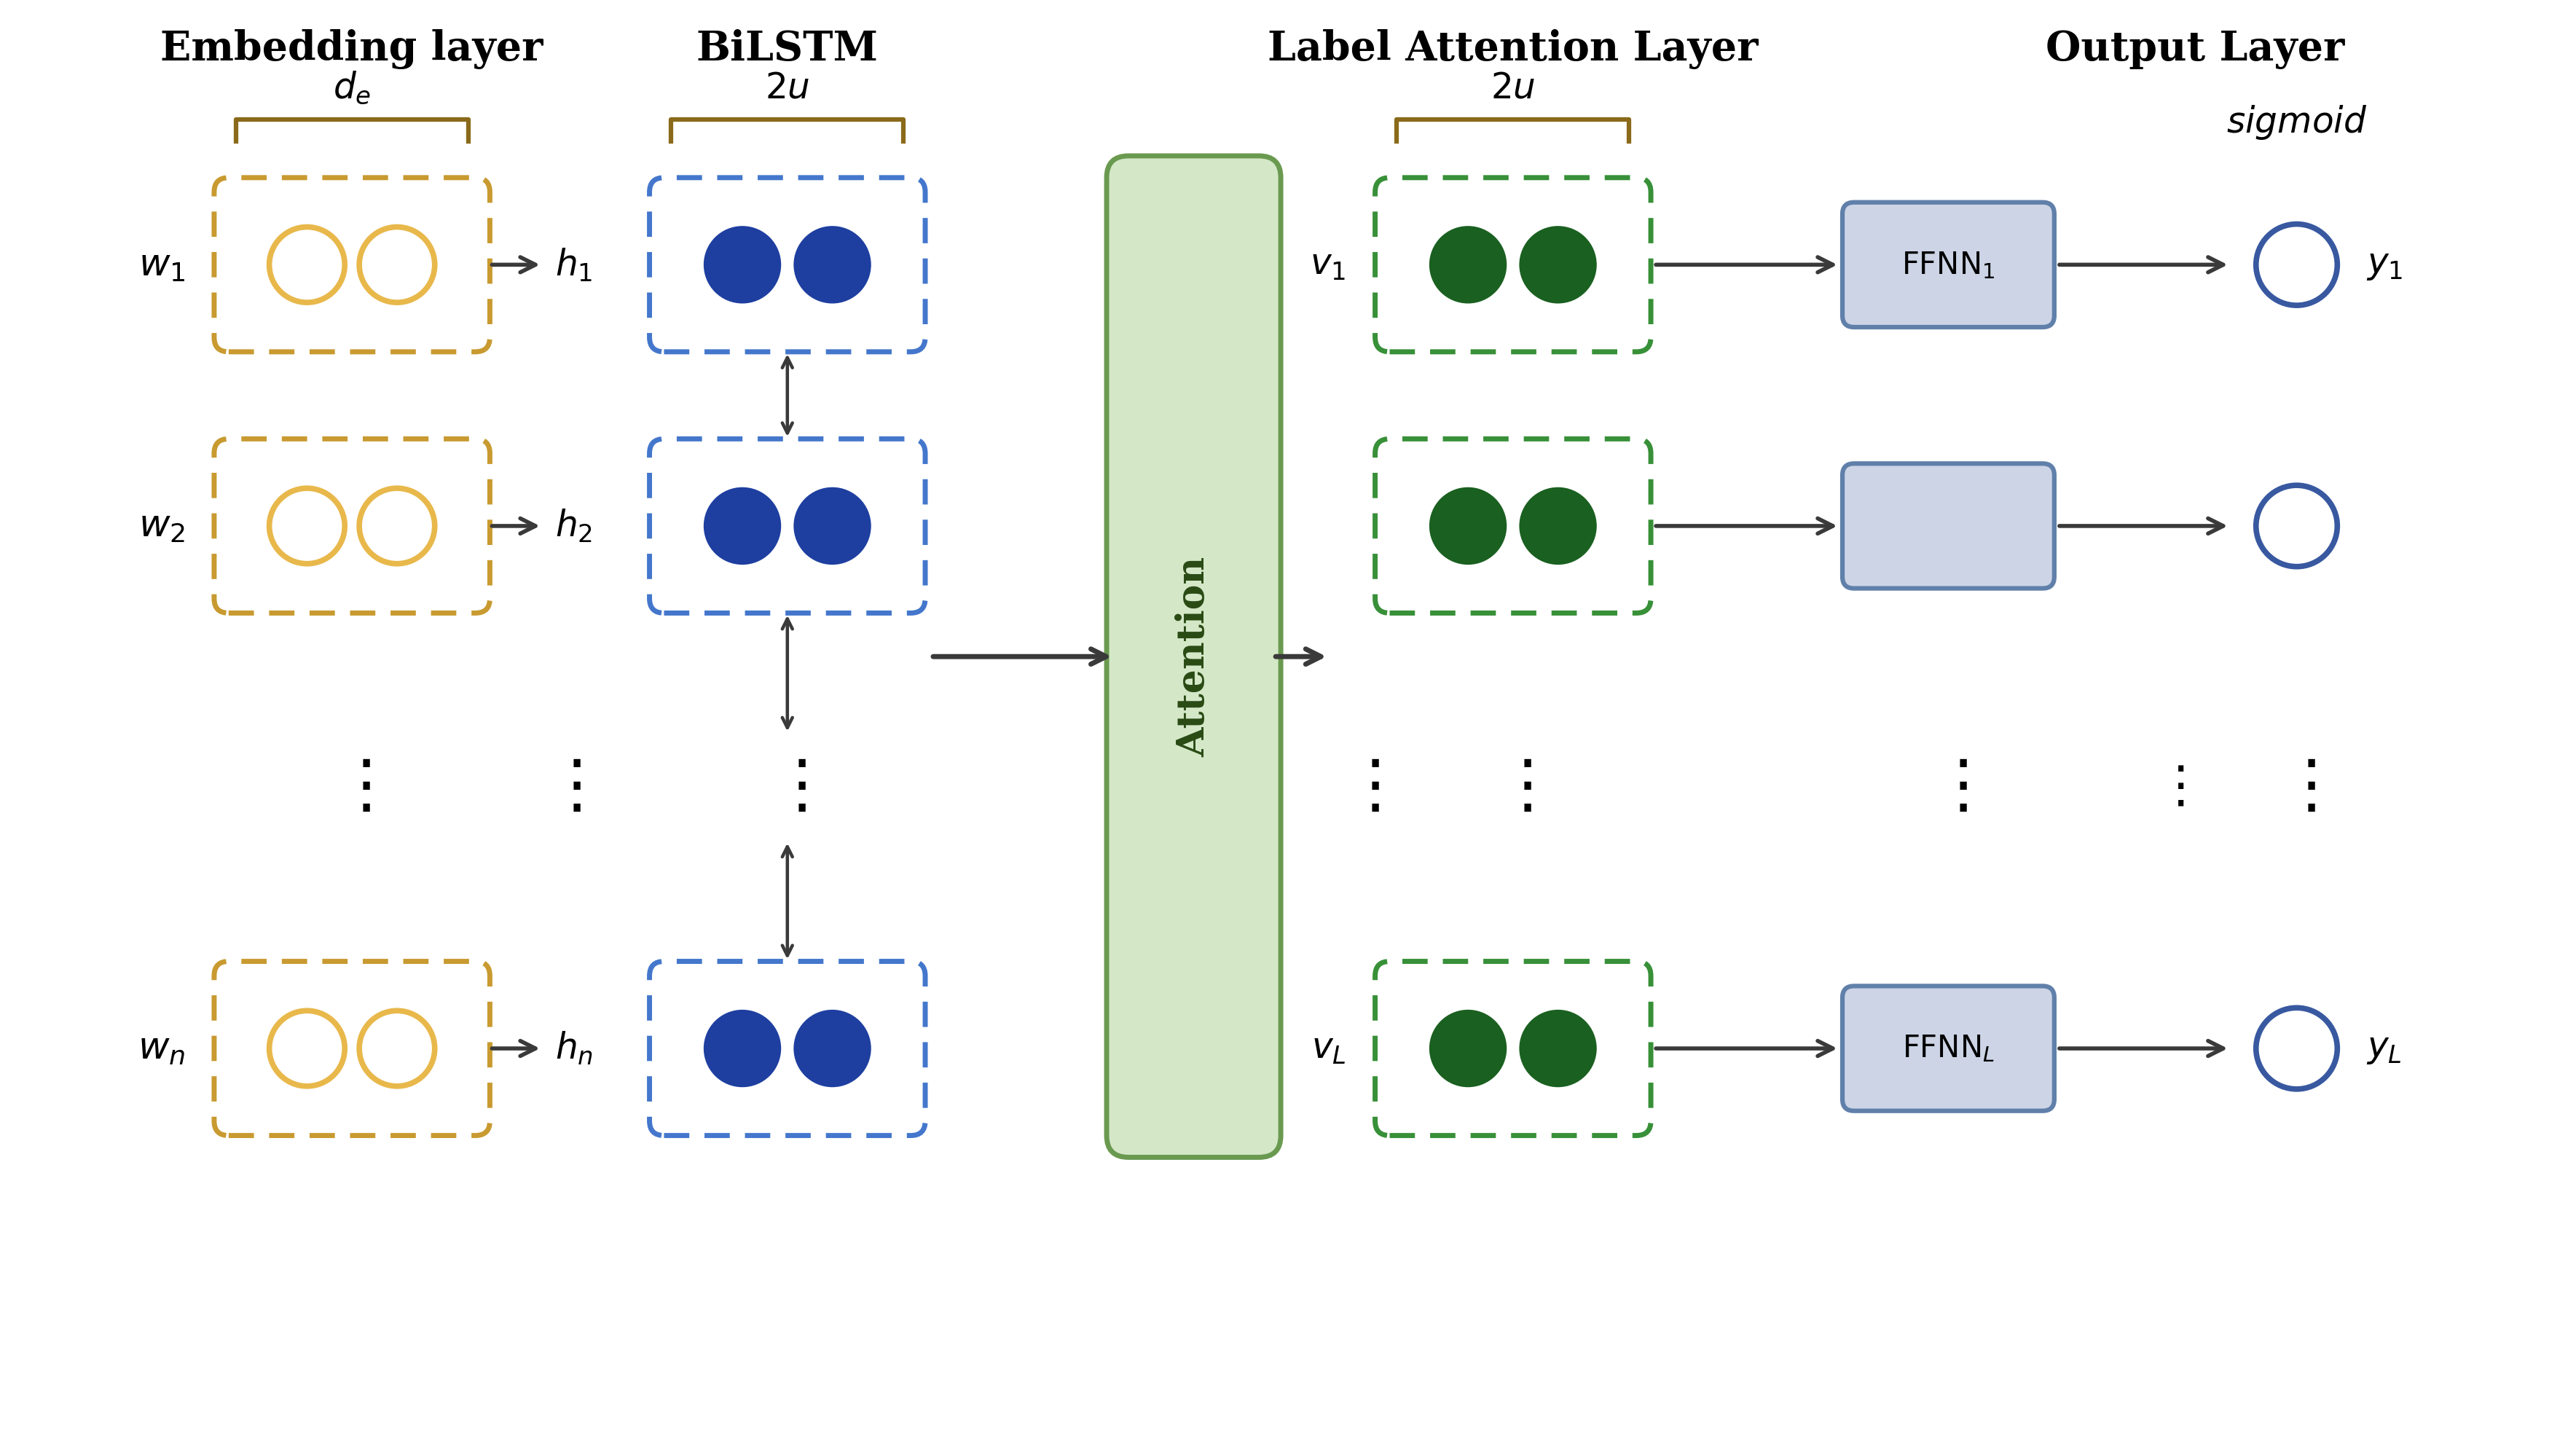
\includegraphics[width=0.75\textwidth]{figures/bilstm_laat_arch.png}
\caption{Architecture of the BiLSTM-LAAT model (Model D), following \citet{vu2020label}. Input word tokens $w_1, \ldots, w_n$ (up to 4,000) are embedded ($d_e\!=\!200$) and encoded by a bidirectional LSTM ($2u\!=\!512$). The label attention mechanism computes $L\!=\!50$ label-specific vectors via learned attention weights, each classified independently through a per-label FFNN with sigmoid activation.}
\label{fig:bilstm_arch}
\end{figure}

\textbf{Training.} AdamW optimizer, $\text{lr} = 10^{-3}$, batch size 32, 10 epochs, focal loss ($\gamma = 2.00$), dropout $p = 0.30$, early stopping with patience 3. \textbf{11,107,506 trainable parameters.}

\textbf{Temperature calibration.} A single scalar parameter $T^*= 0.63$ is fitted on the validation set, reducing expected calibration error from 0.07 to 0.02.

\textbf{Training progression (BiLSTM-LAAT):}

\begin{table}[H]
\centering
\caption{BiLSTM-LAAT (Model D) training progression.}
\label{tab:train_d}
\small
\begin{tabular}{ccc}
\toprule
\textbf{Epoch} & \textbf{Train Loss} & \textbf{Val Micro-F1} \\
\midrule
1  & 0.03 & 0.67 \\
2  & 0.02 & 0.69 \\
3  & 0.02 & 0.71 \\
4  & 0.02 & 0.71 \\
5  & 0.02 & 0.71 \\
6  & 0.01 & 0.72 \\
7  & 0.01 & 0.72 \\
8  & 0.01 & 0.72 \\
9  & 0.01 & 0.72 \\
10 & 0.01 & \textbf{0.72} \\
\bottomrule
\end{tabular}
\end{table}

\subsection{Ensemble Methods}

We combine models by averaging their predicted probabilities with learned weights: $\mathbf{P}_{\text{ens}} = \sum_i w_i \cdot \mathbf{P}_i$, where $\sum_i w_i = 1$. Both the weights and the global decision threshold are tuned jointly on the validation set:

\begin{table}[H]
\centering
\caption{Ensemble configurations with validation-tuned weights and thresholds.}
\label{tab:ensemble_weights}
\small
\begin{tabular}{llccccl}
\toprule
\textbf{Variant} & \textbf{Components} & $w_{\text{TF}}$ & $w_{\text{CB1}}$ & $w_{\text{CB2}}$ & $w_{\text{BL}}$ & \textbf{Thr.} \\
\midrule
v1 & TF-IDF + Chunk-BERT v1          & 0.65 & 0.35 & --  & --  & 0.63 \\
v2 & TF-IDF + Chunk-BERT v2          & 0.35 & --  & 0.65 & --  & 0.43 \\
v3 & TF-IDF + Chunk-BERT v1 + v2     & 0.30 & 0.00 & 0.70 & --  & 0.40 \\
\rowcolor{lightgray}
v4 & TF-IDF + BiLSTM-LAAT            & 0.15 & --  & --  & 0.85 & 0.35 \\
v5 & TF-IDF + Chunk-BERT v2 + BiLSTM & 0.10 & --  & 0.30 & 0.60 & 0.35 \\
\bottomrule
\end{tabular}

\vspace{4pt}
\parbox{0.9\textwidth}{\footnotesize TF = TF-IDF+SGD, CB = Chunk-BERT, BL = BiLSTM-LAAT. \textbf{v4 is the best ensemble.}}
\end{table}

\subsection{Hyperparameter Summary}

\begin{table}[H]
\centering
\caption{Hyperparameter comparison across all models.}
\label{tab:hyperparams}
\small
\begin{tabular}{lcccc}
\toprule
\textbf{Hyperparameter} & \textbf{TF-IDF+SGD} & \textbf{ClinicalBERT} & \textbf{Chunk-BERT} & \textbf{BiLSTM-LAAT} \\
\midrule
Encoder          & TF-IDF         & Bio\_ClinicalBERT  & Bio\_ClinicalBERT  & BiLSTM \\
Parameters       & 2,500,000      & 108,000,000        & 108,000,000        & 11,107,506 \\
Max tokens       & 50K features   & 512                & 3,072 (6$\times$512)    & 4,000 \\
Learning rate    & N/A            & $2\!\times\!10^{-5}$ & $10^{-3}$ / $2\!\times\!10^{-5}$ & $10^{-3}$ \\
Batch size       & Full dataset   & 32                 & 4 $\times$ 8 = 32  & 32 \\
Epochs           & 100 iter.      & 3                  & 5 + 7              & 10 \\
Loss             & Log loss       & BCE                & Focal ($\gamma\!=\!2.00$) & Focal ($\gamma\!=\!2.00$) \\
Dropout          & --            & 0.10               & 0.10               & 0.30 \\
Optimizer        & SGD            & AdamW              & AdamW              & AdamW \\
Train time       & 2 min (CPU)    & 1.50 hr (L4)       & 8 hr (L4)          & 30 min (L4) \\
Val Micro-F1     & 0.58           & 0.47               & 0.47               & \textbf{0.72} \\
\bottomrule
\end{tabular}
\end{table}

% ══════════════════════════════════════════════════════════════════════
% 5. RESULTS
% ══════════════════════════════════════════════════════════════════════
\section{Results}

\subsection{Main Results}

Figure \ref{fig:comparison_bars} and Table \ref{tab:main_results} summarize test-set performance across all models and ensembles ($n = 18{,}852$, top-50 codes).

\begin{figure}[H]
    \centering
    
\includegraphics[width=0.80\textwidth,height=6cm]{figures/model_comparison_bars.png}
    \caption{Metric comparison across all models and ensemble variants.}
    \label{fig:comparison_bars}
\end{figure}

The standout result is BiLSTM-LAAT: with only 11.10M parameters it reaches Micro-F1 = 0.72, beating TF-IDF+SGD by 0.12 points and truncated ClinicalBERT by 0.20. Ensemble v4 (85\% BiLSTM-LAAT, 15\% TF-IDF) does not improve Micro-F1 further but nudges Macro-F1 up to 0.67, suggesting the TF-IDF component helps on a few tail codes.

A few other patterns are worth noting. TF-IDF + SGD has the highest recall of any single model (0.75), which makes sense given that ICD codes often boil down to specific medical terms that bigram features capture well. Truncated ClinicalBERT, on the other hand, is the weakest model across the board (Micro-F1 = 0.52), confirming that chopping off most of the note is a dealbreaker. Chunk-BERT v2 with focal loss goes the other way, achieving the highest precision (0.79) but at the expense of recall (0.42), because focal loss pushes the model to only predict codes it is very confident about. Finally, the AUROC of 0.95 for Ensemble v4 indicates strong ranking ability; the gap between AUROC and F1 suggests that per-label threshold tuning could close some of the remaining performance gap.

\begin{table}[H]
\centering
\caption{Test-set results for all models and ensembles (Top-50, $n\!=\!18{,}852$). Best in \textbf{bold}.}
\label{tab:main_results}
\small
\resizebox{\textwidth}{!}{%
\begin{tabular}{l c c c c c c c}
\toprule
\textbf{Model} & \textbf{Thr.} & \textbf{Mi-F1} & \textbf{Ma-F1} & \textbf{Mi-P} & \textbf{Mi-R} & \textbf{Ma-AUP} & \textbf{Mi-AUC} \\
\midrule
\multicolumn{8}{l}{\textit{Individual Models}} \\
\midrule
TF-IDF + SGD (Model A)         & 0.53 & 0.60 & 0.57 & 0.49 & 0.75 & 0.57 & 0.93 \\
ClinicalBERT (Model B)         & 0.28 & 0.52 & 0.44 & 0.52 & 0.52 & 0.45 & 0.87 \\
Chunk-BERT v1 (Model C)        & 0.63 & 0.53 & 0.50 & 0.42 & 0.72 & 0.52 & 0.89 \\
Chunk-BERT v2 / Focal          & 0.05 & 0.55 & 0.43 & 0.79 & 0.42 & 0.56 & 0.92 \\
\rowcolor{lightgray}
\textbf{BiLSTM-LAAT (Model D)} & \textbf{0.30} & \textbf{0.72} & \textbf{0.66} & 0.72 & 0.72 & 0.68 & 0.95 \\
\midrule
\multicolumn{8}{l}{\textit{Ensemble Models}} \\
\midrule
Ens.\ v1 (TF-IDF + CB\,v1)         & 0.63 & 0.62 & 0.59 & 0.57 & 0.69 & 0.59 & 0.93 \\
Ens.\ v2 (TF-IDF + CB\,v2)         & 0.43 & 0.53 & 0.40 & 0.81 & 0.39 & 0.61 & 0.94 \\
Ens.\ v3 (TF-IDF + CB\,v1+v2)      & 0.40 & 0.53 & 0.40 & 0.81 & 0.39 & 0.61 & 0.94 \\
\rowcolor{lightgray}
\textbf{Ens.\ v4 (TF-IDF + BiLSTM)} & \textbf{0.35} & \textbf{0.72} & \textbf{0.67} & 0.72 & 0.72 & \textbf{0.69} & \textbf{0.95} \\
Ens.\ v5 (TF-IDF + CB\,v2 + BiLSTM) & 0.35 & 0.69 & 0.61 & \textbf{0.80} & 0.62 & 0.68 & \textbf{0.95} \\
\bottomrule
\end{tabular}}
\vspace{2pt}

{\footnotesize Mi = Micro, Ma = Macro, P = Precision, R = Recall, AUP = AUPRC, AUC = AUROC. CB = Chunk-BERT.}
\end{table}

\subsection{Training Curves}

Figure \ref{fig:training_curves_detail} plots the training loss and validation F1 over time for Chunk-BERT v1 and BiLSTM-LAAT. The two models behave quite differently: BiLSTM-LAAT's loss falls steadily across all 10 epochs, while Chunk-BERT shows a clear kink at epoch 6 when we unfreeze the last two BERT layers.

\begin{figure}[H]
    \centering
    \begin{subfigure}[b]{0.48\textwidth}
        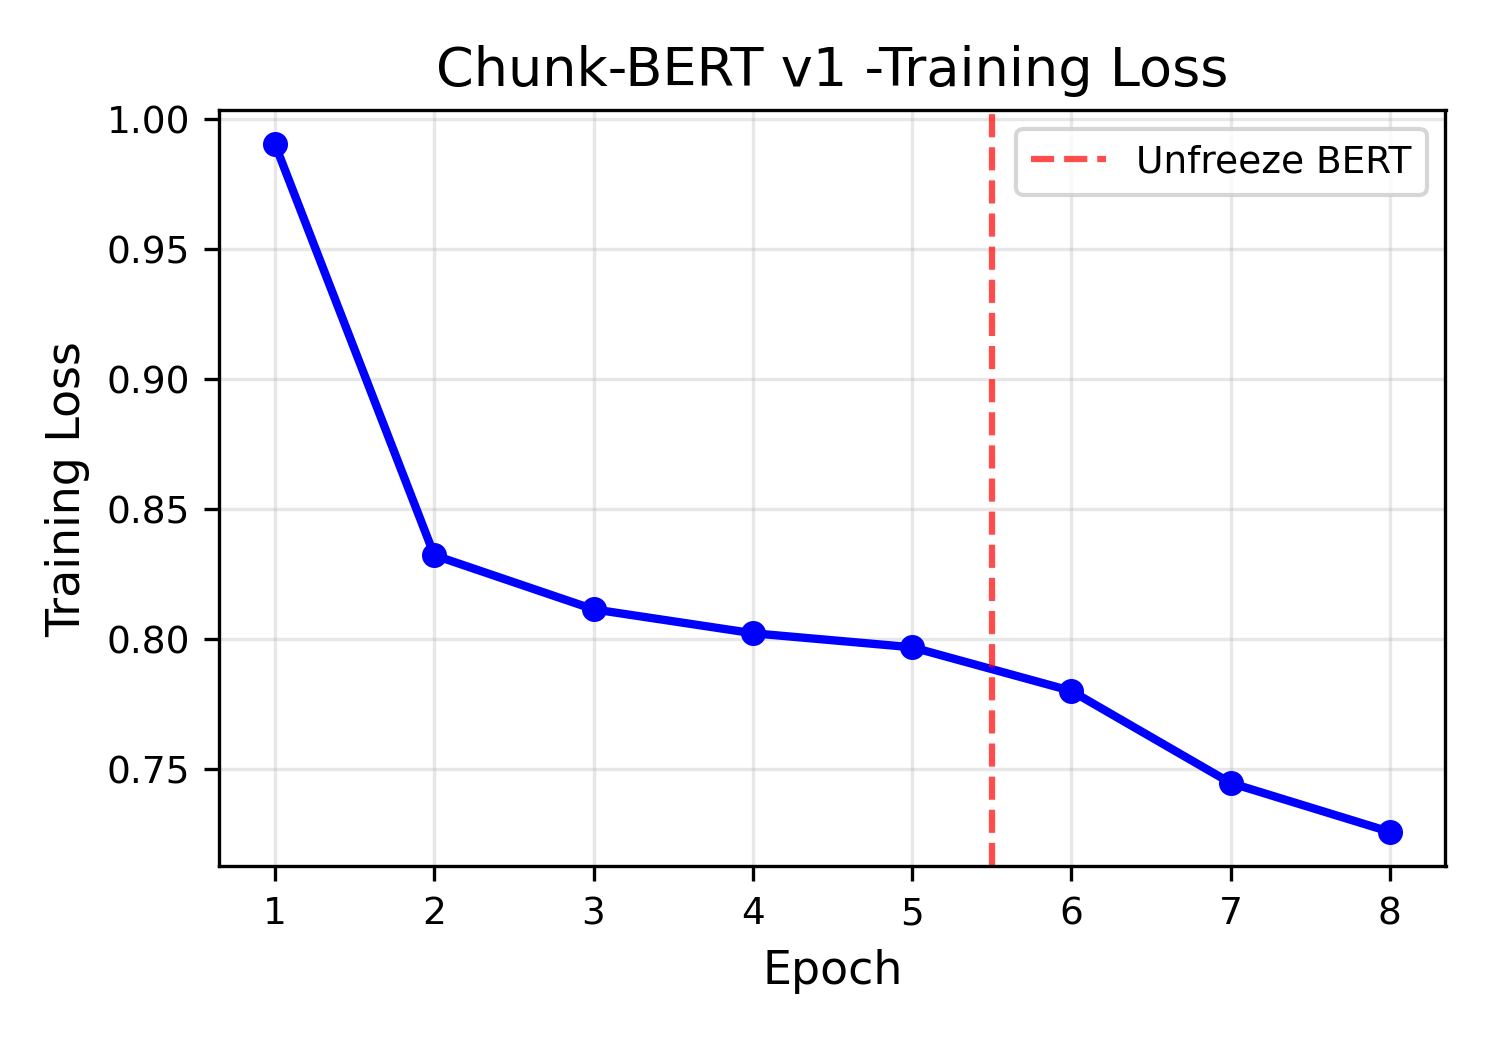
\includegraphics[width=\textwidth]{figures/training_loss_c.png}
        \caption{Chunk-BERT v1 training loss}
    \end{subfigure}
    \hfill
    \begin{subfigure}[b]{0.48\textwidth}
        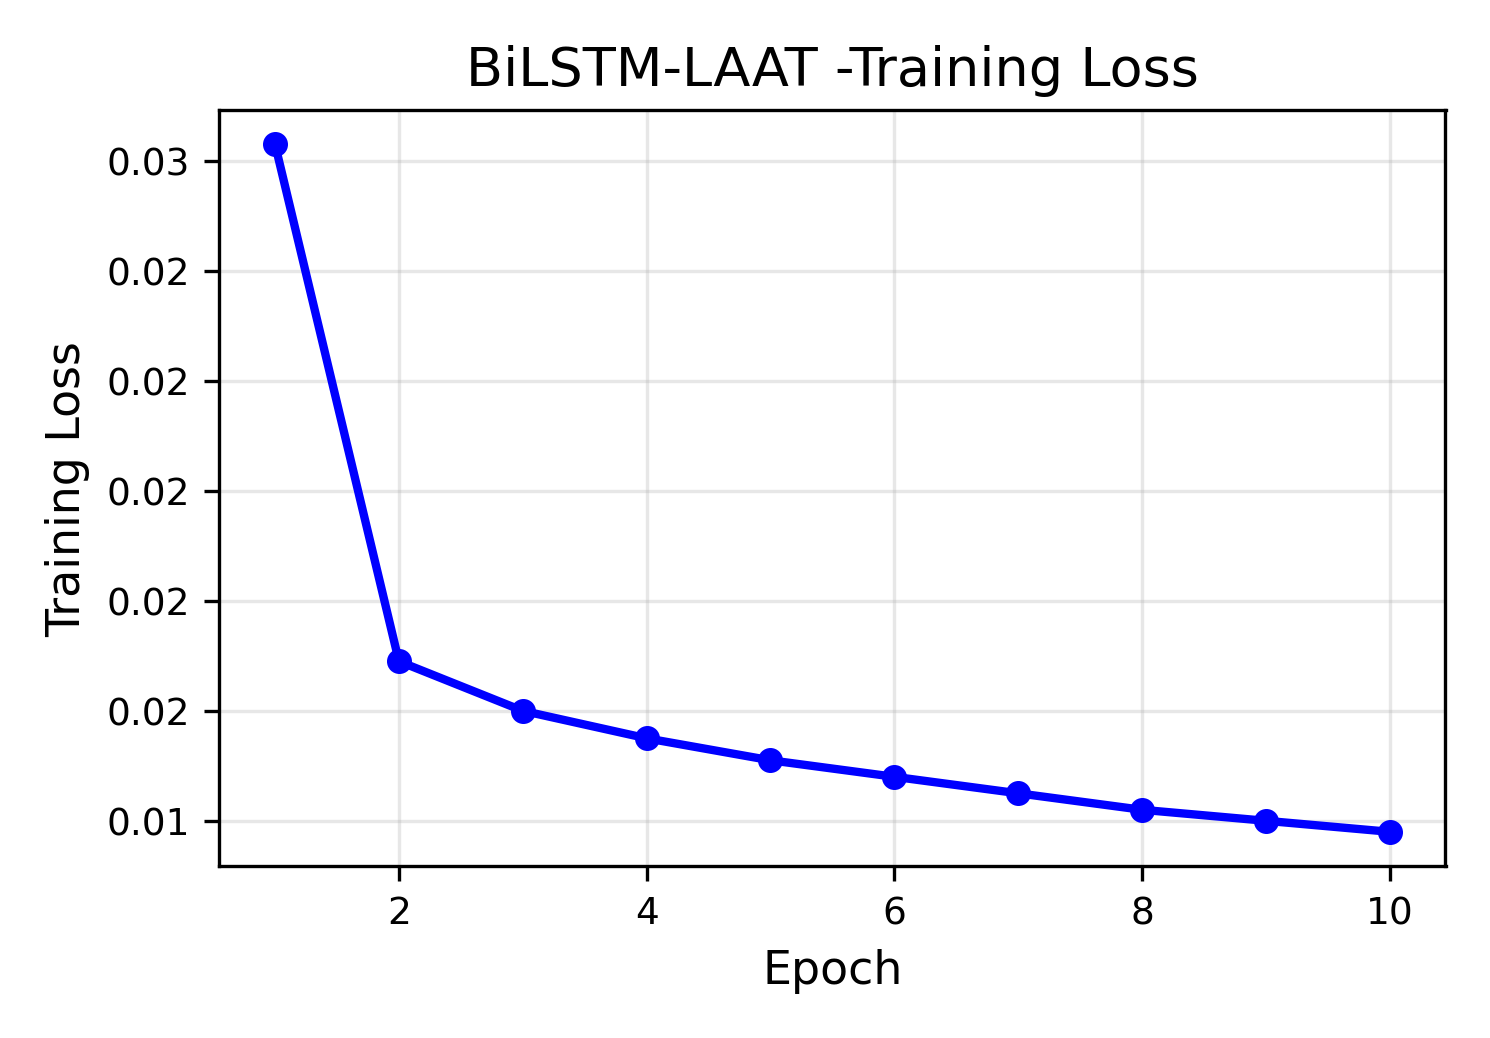
\includegraphics[width=\textwidth]{figures/training_loss_d.png}
        \caption{BiLSTM-LAAT training loss}
    \end{subfigure}
    \\[6pt]
    \begin{subfigure}[b]{0.48\textwidth}
        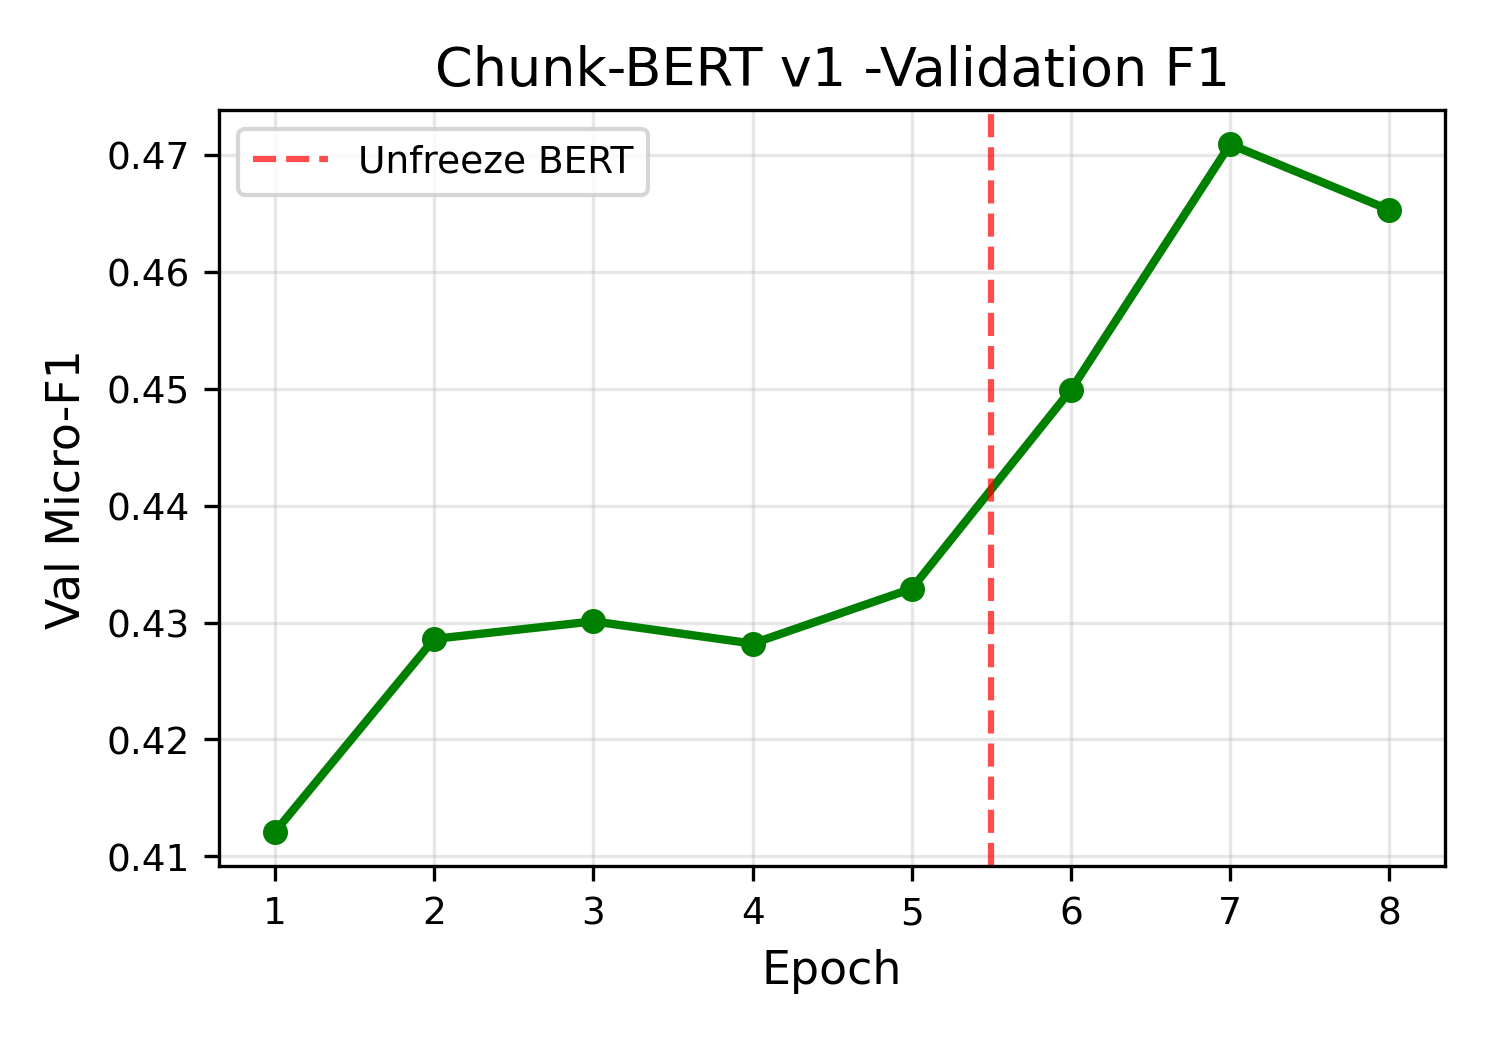
\includegraphics[width=\textwidth]{figures/training_f1_c.png}
        \caption{Chunk-BERT v1 validation F1}
    \end{subfigure}
    \hfill
    \begin{subfigure}[b]{0.48\textwidth}
        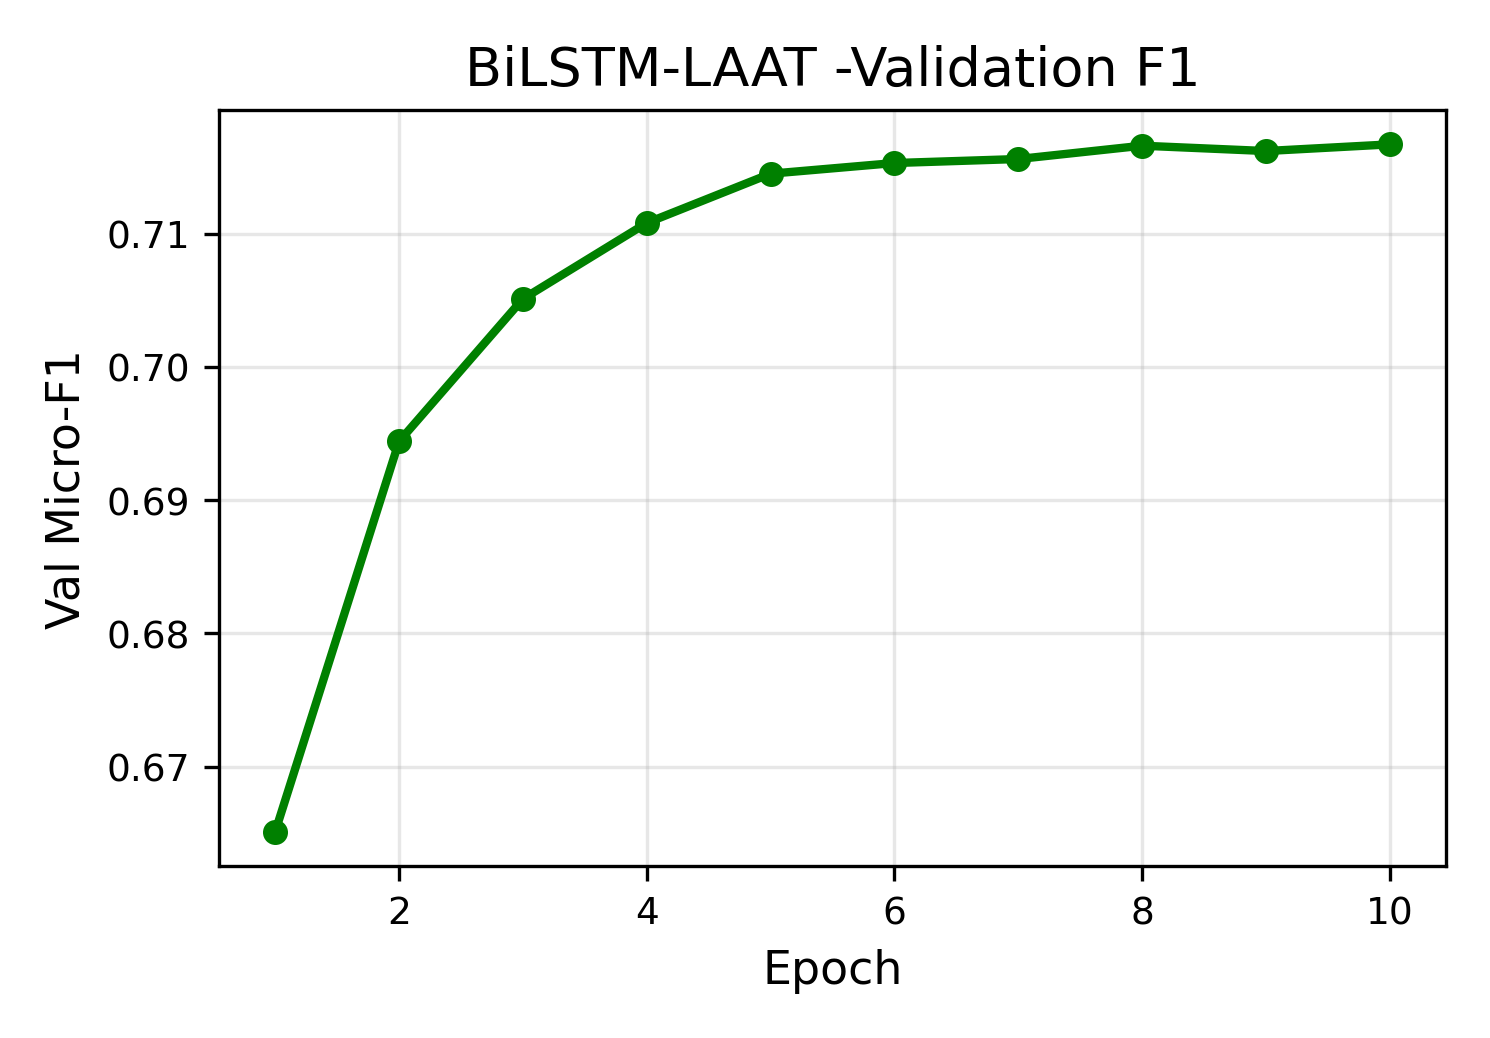
\includegraphics[width=\textwidth]{figures/training_f1_d.png}
        \caption{BiLSTM-LAAT validation F1}
    \end{subfigure}
    \caption{Detailed training curves. BiLSTM-LAAT achieves faster and more stable convergence, while Chunk-BERT shows a two-phase pattern with an inflection at epoch 6 when BERT layers are unfrozen.}
    \label{fig:training_curves_detail}
\end{figure}

Looking at the curves in more detail, BiLSTM-LAAT's loss drops from 0.03 to 0.01 across 10 epochs while validation F1 climbs from 0.67 to 0.72. The trajectory is still gently improving at epoch 10, so more training might squeeze out a bit more. For Chunk-BERT v1, validation F1 stalls around 0.43 during the frozen phase (epochs 1 to 5). The moment we unfreeze the BERT layers at epoch 6, F1 jumps to 0.45 and peaks at 0.47 by epoch 7, after which early stopping kicks in. This makes it clear that end-to-end fine-tuning matters a lot for the chunked setup. Chunk-BERT v2 with focal loss ($\gamma = 2.00$) converges faster early on but trades recall for precision; its optimal threshold ends up at just 0.05, a sign that the model's probability outputs are tightly clustered near zero for most codes.

\subsection{Per-Label Confusion Matrices}

Figures \ref{fig:confusion_baseline} through \ref{fig:confusion_ens} show per-label confusion matrices for the 10 most frequent codes. TF-IDF picks up most frequent codes but sprays false positives, ClinicalBERT misses many codes entirely because it never sees the relevant text, and BiLSTM-LAAT has the most even balance between true positives and false negatives regardless of code frequency.

\begin{figure}[H]
    \centering
    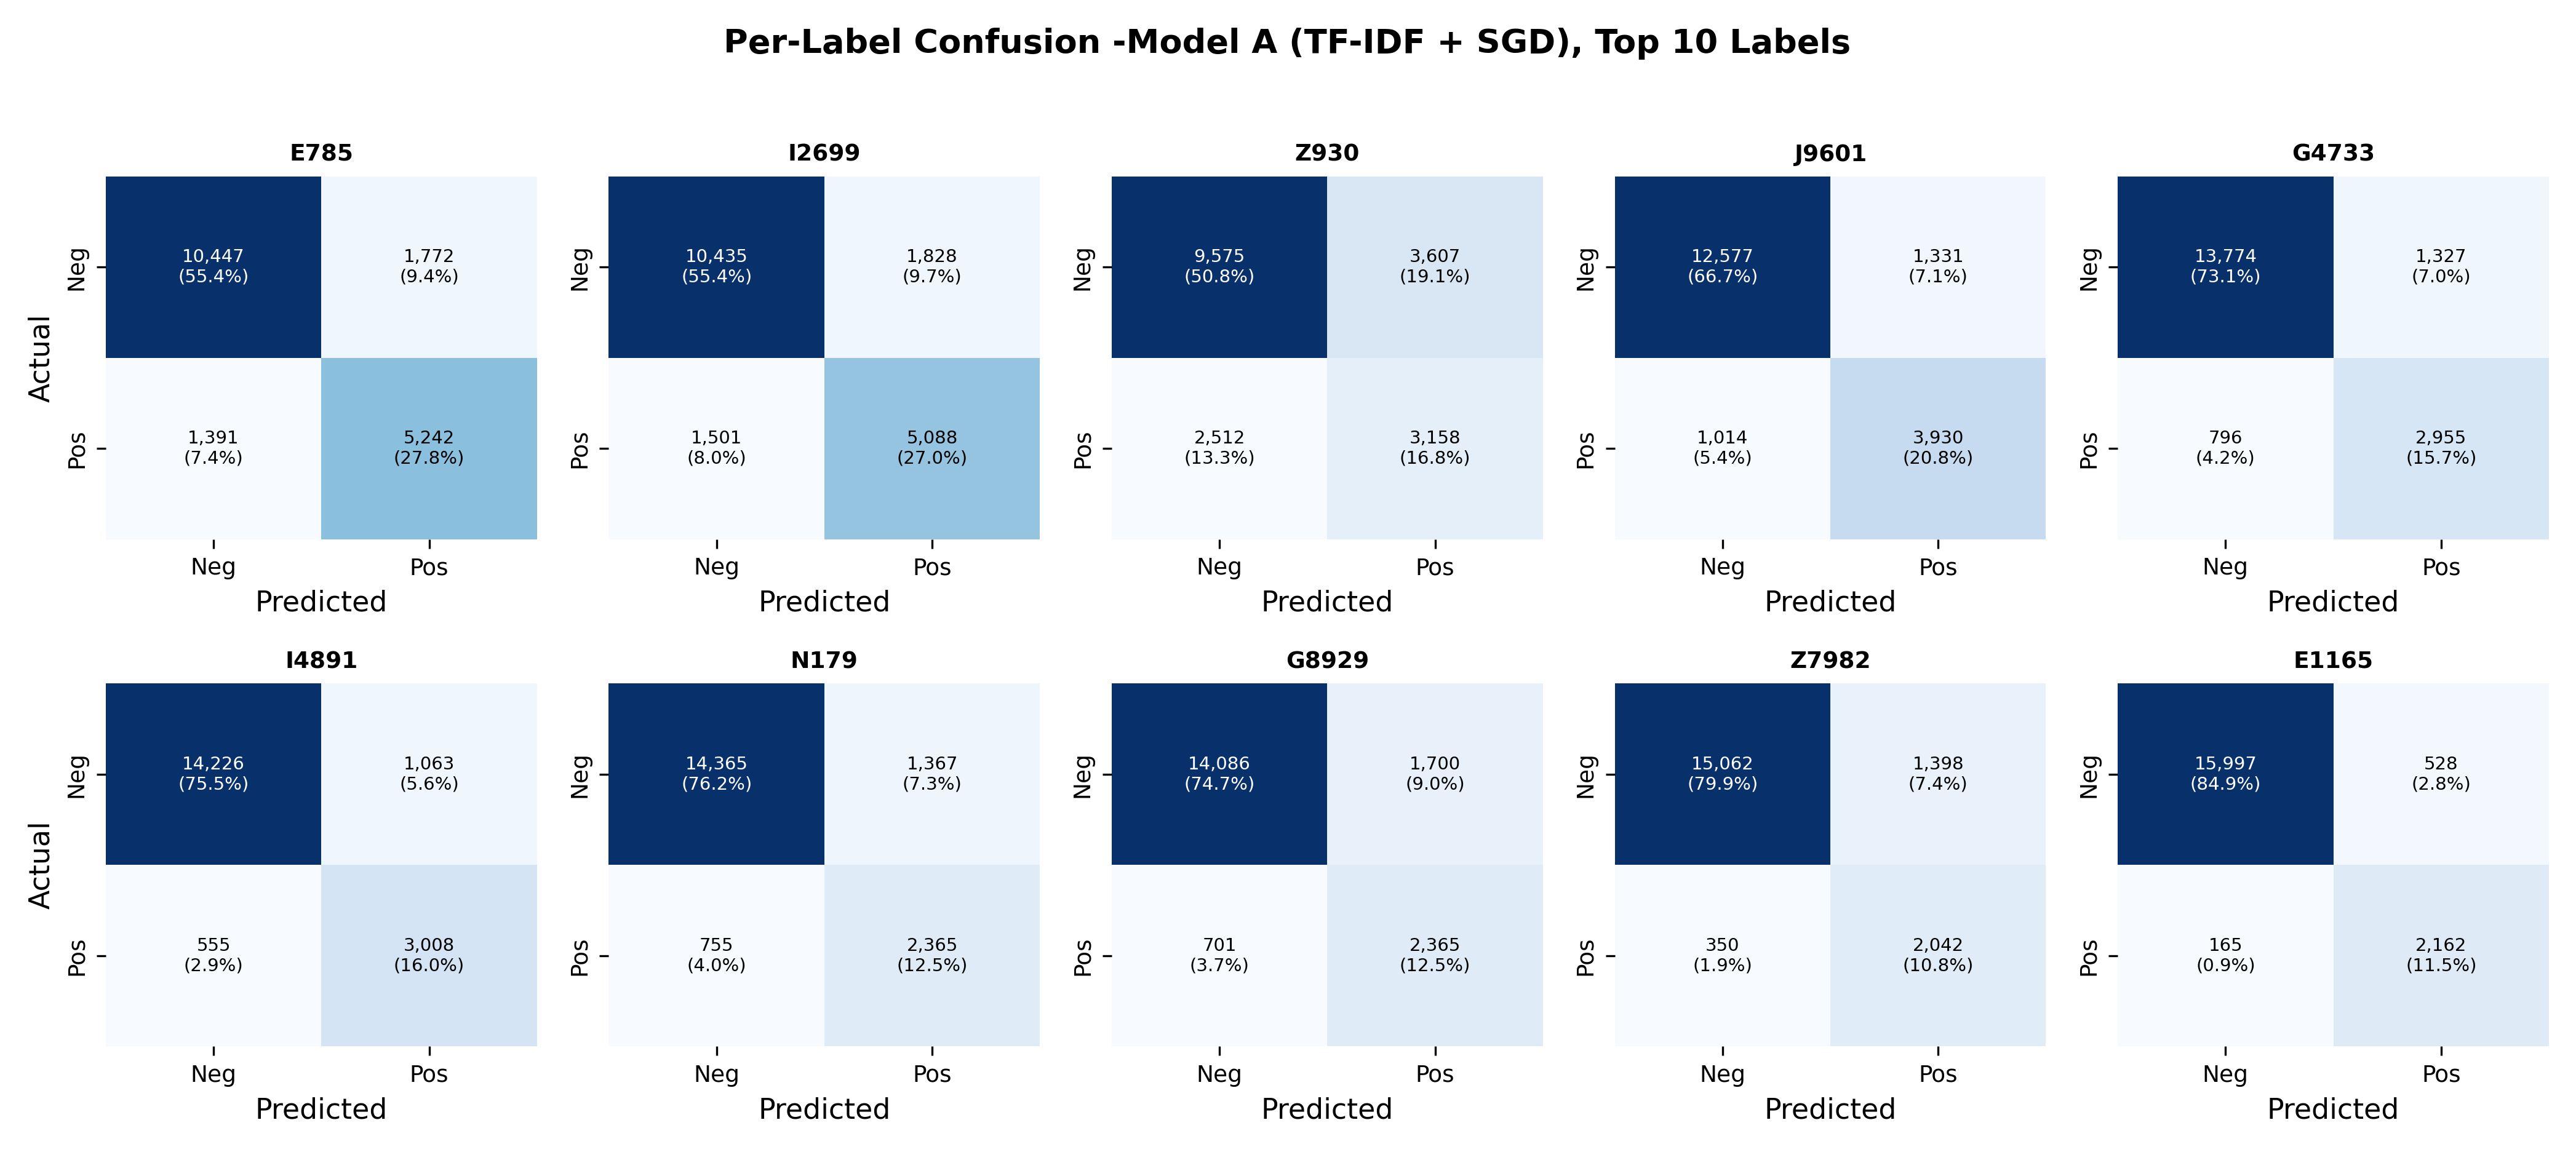
\includegraphics[width=\textwidth]{figures/confusion_matrix_a.png}
    \caption{Per-label confusion matrix (top-10 codes) for TF-IDF + SGD (Model A).}
    \label{fig:confusion_baseline}
\end{figure}
\vspace{-6pt}
\begin{figure}[H]
    \centering
    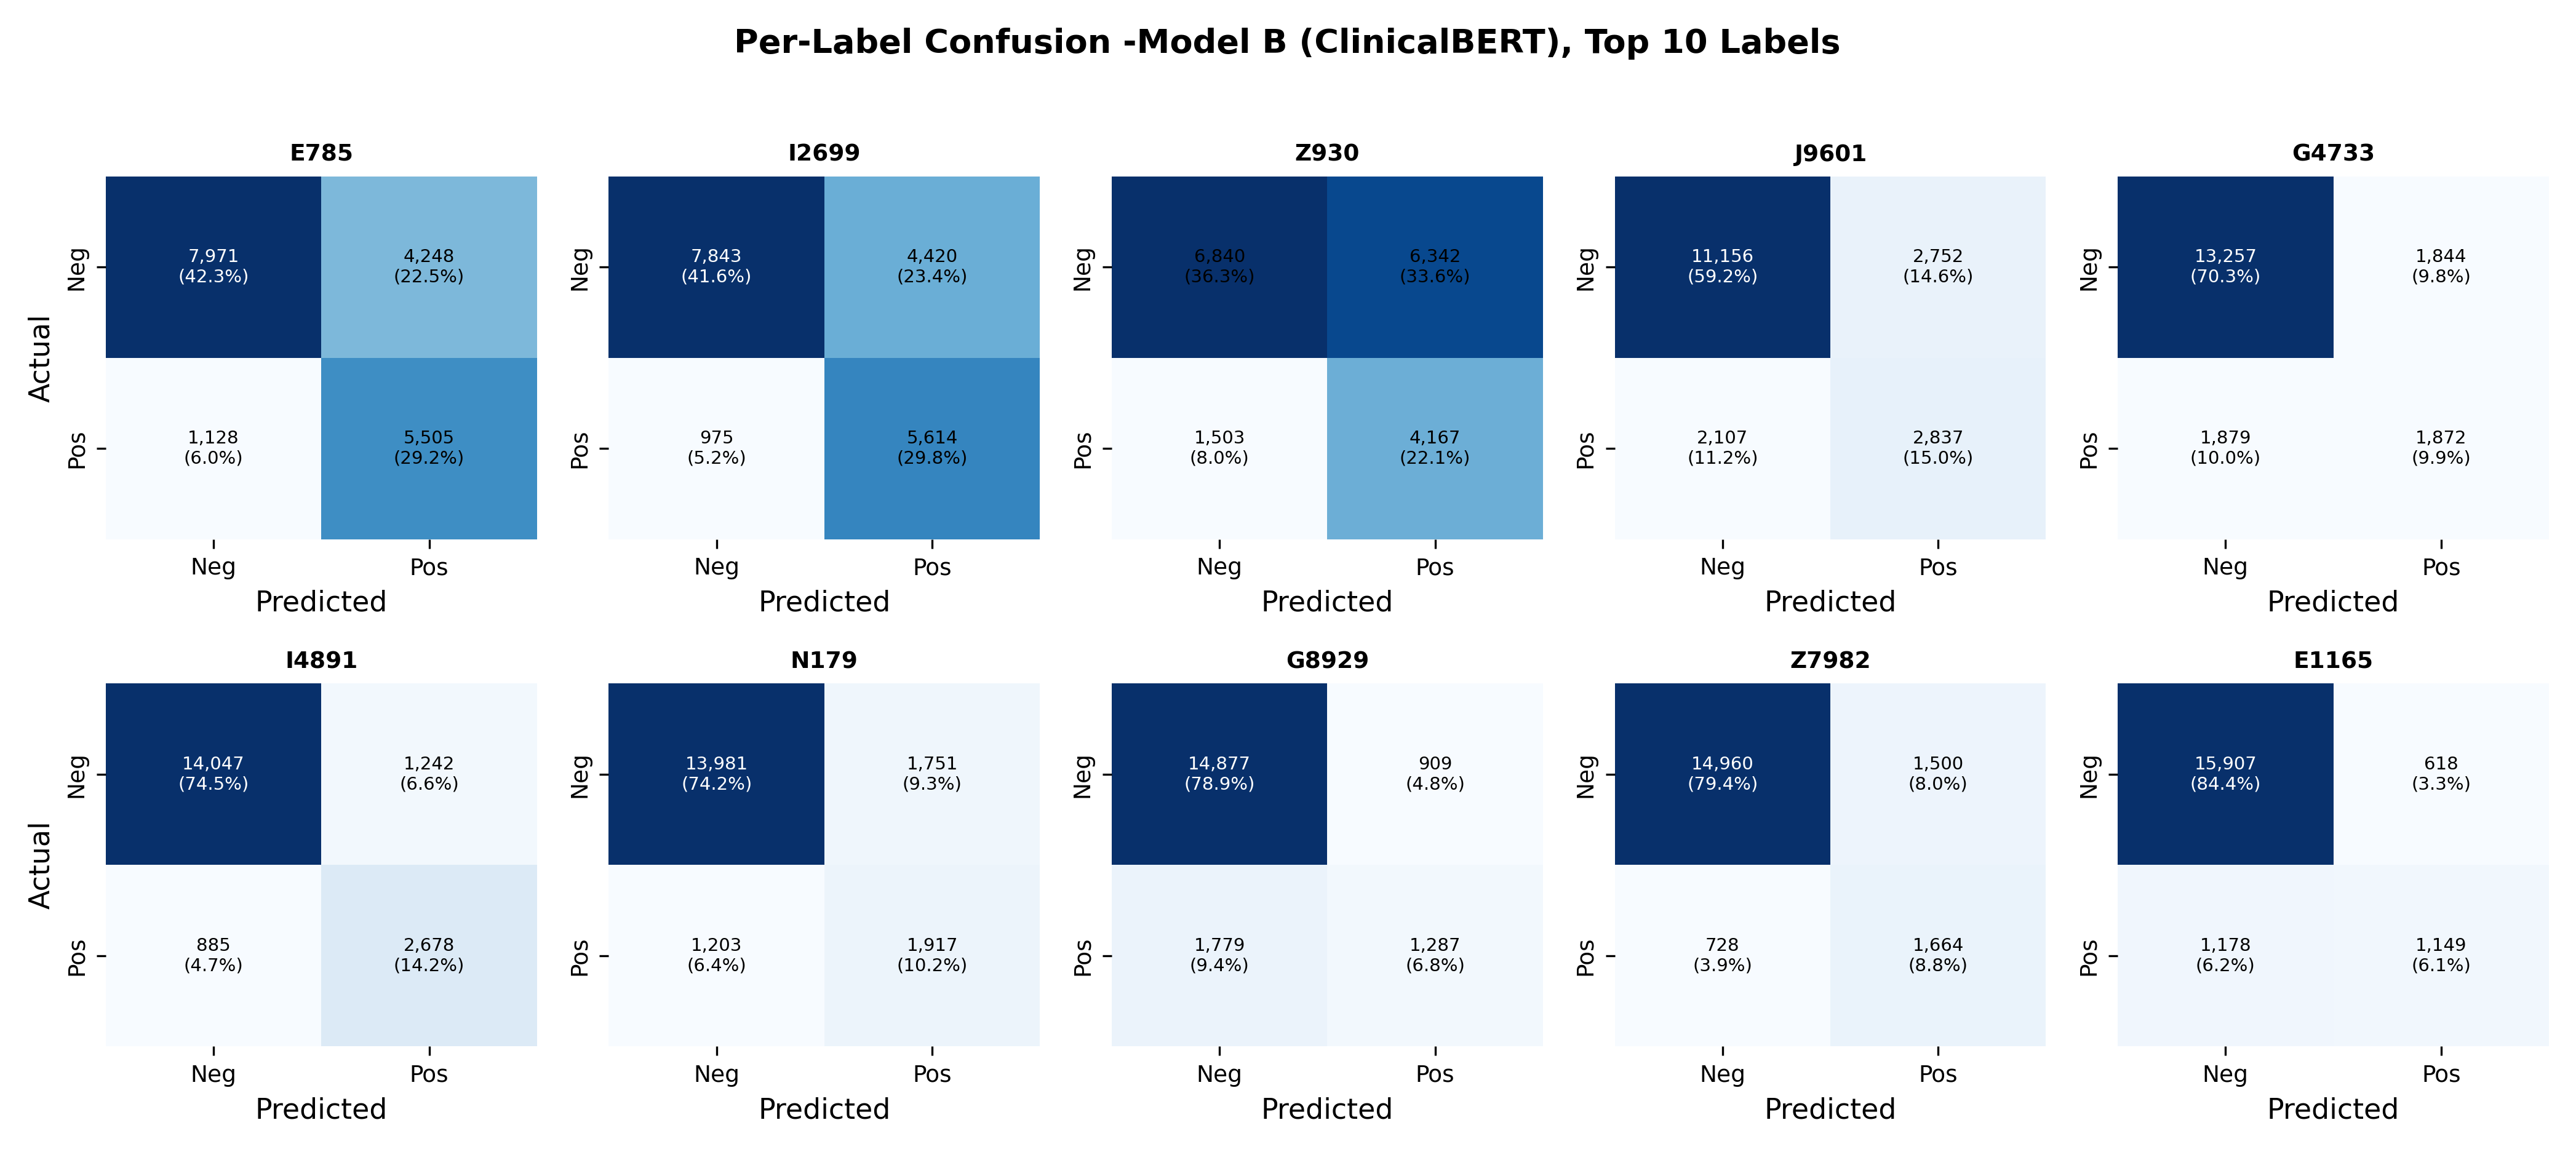
\includegraphics[width=\textwidth]{figures/confusion_matrix_b.png}
    \caption{Per-label confusion matrix for ClinicalBERT (Model B). Struggles with rare codes due to truncation.}
    \label{fig:confusion_b}
\end{figure}

\clearpage

\begin{figure}[H]
    \centering
    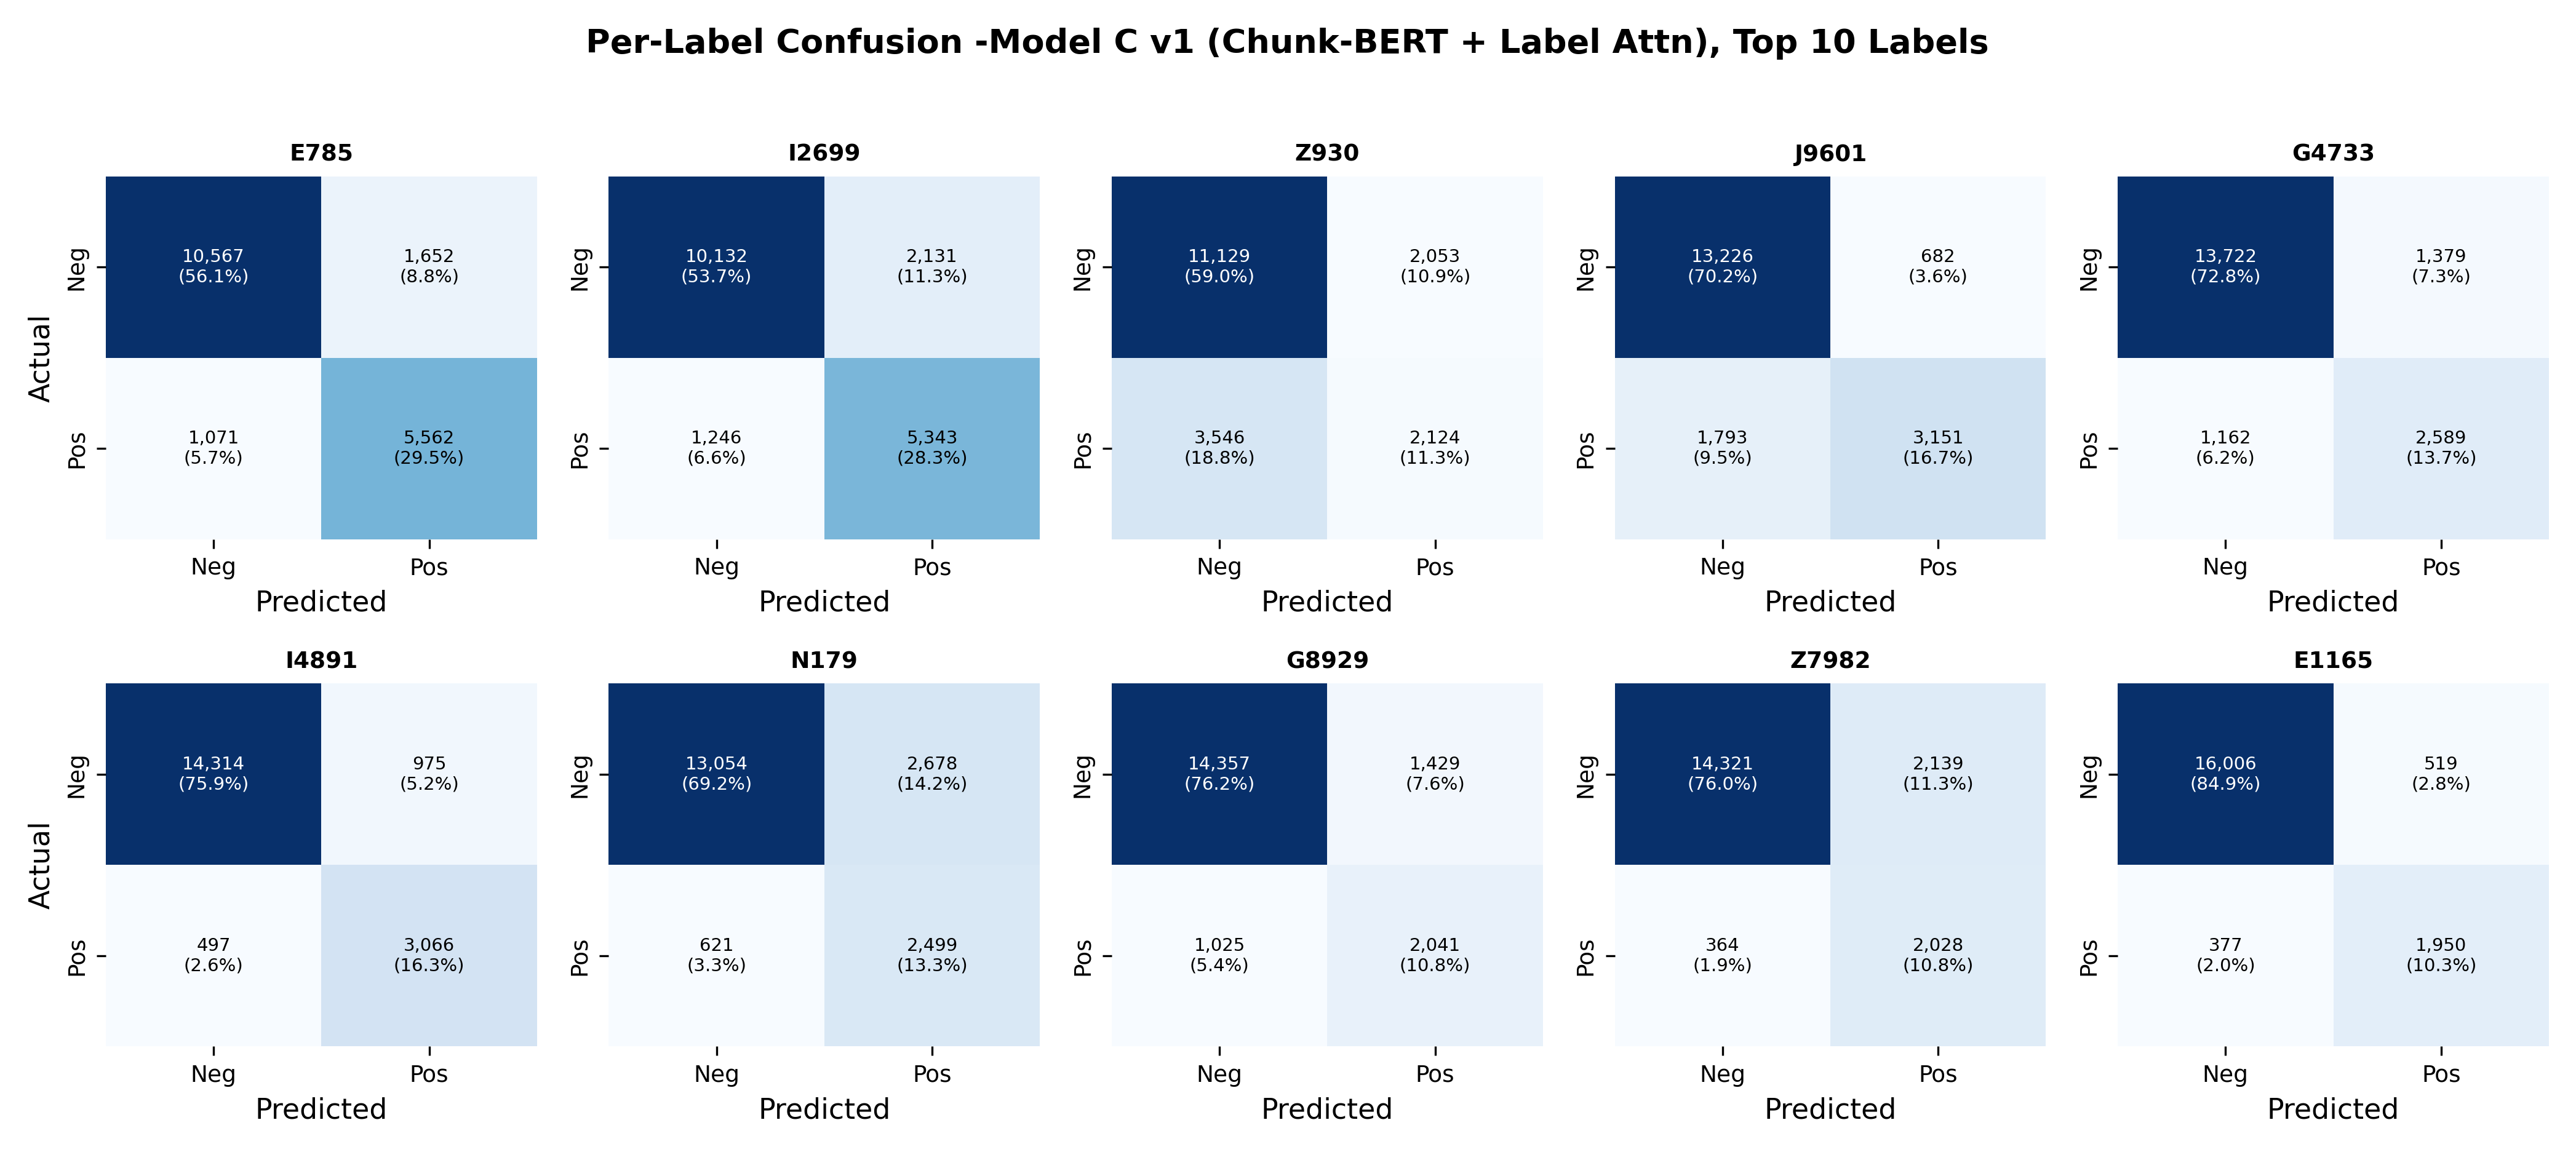
\includegraphics[width=\textwidth]{figures/confusion_matrix_c.png}
    \caption{Per-label confusion matrix for Chunk-BERT v1 (Model C).}
    \label{fig:confusion_approaches}
\end{figure}
\vspace{-6pt}
\begin{figure}[H]
    \centering
    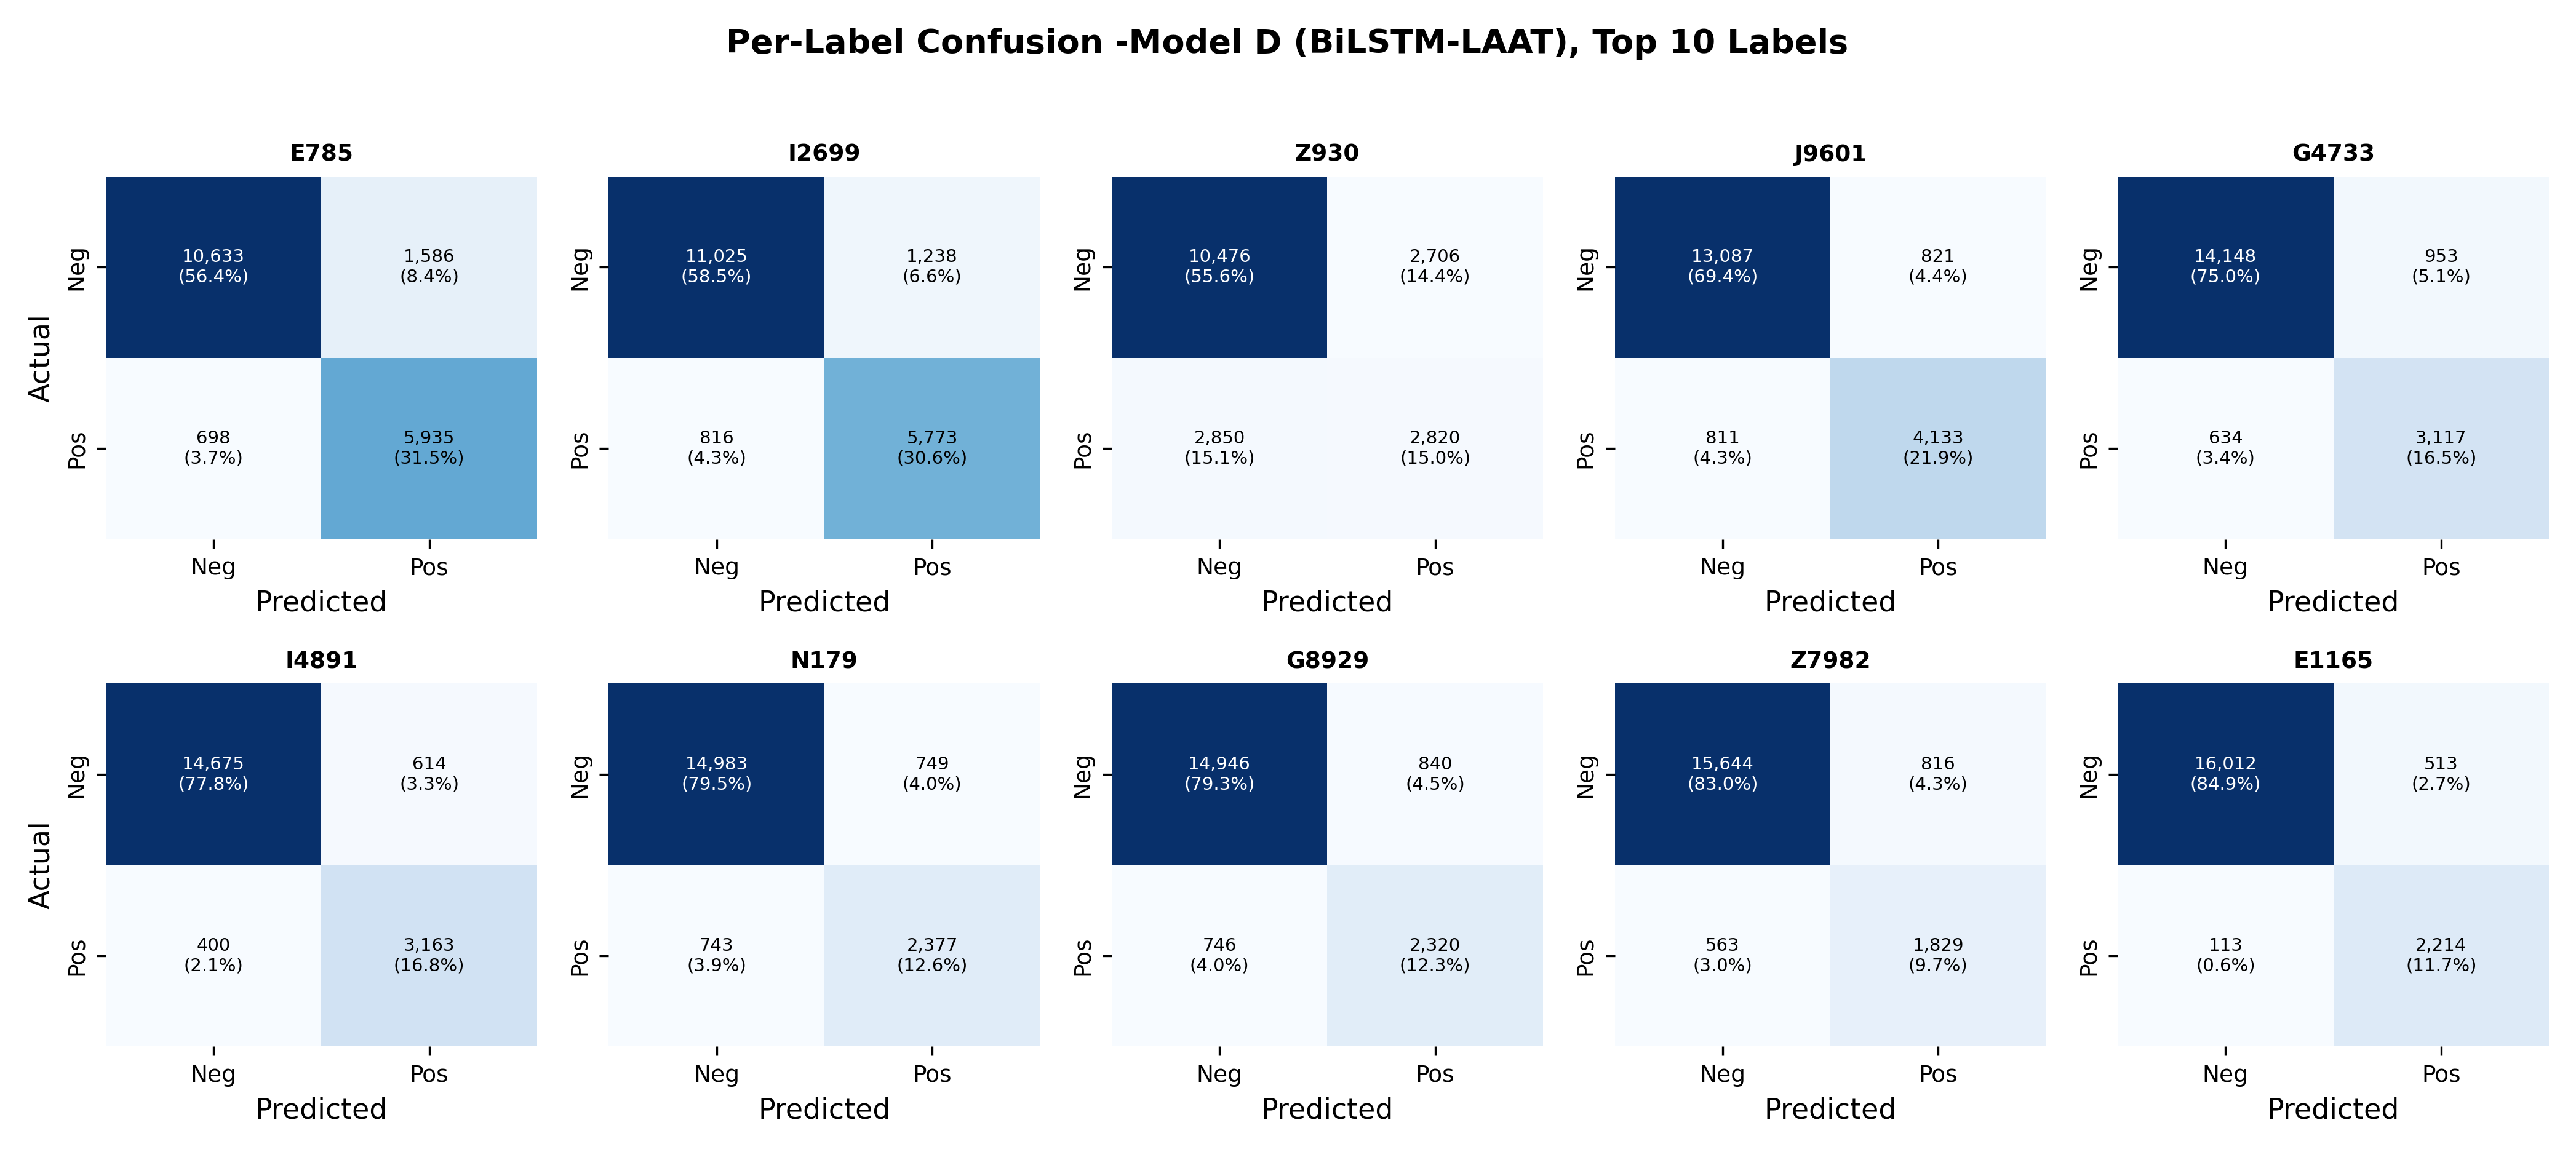
\includegraphics[width=\textwidth]{figures/confusion_matrix_d.png}
    \caption{Per-label confusion matrix for BiLSTM-LAAT (Model D). Most balanced TP/FN ratios across all frequency tiers.}
    \label{fig:confusion_d}
\end{figure}

\clearpage

\begin{figure}[H]
    \centering
    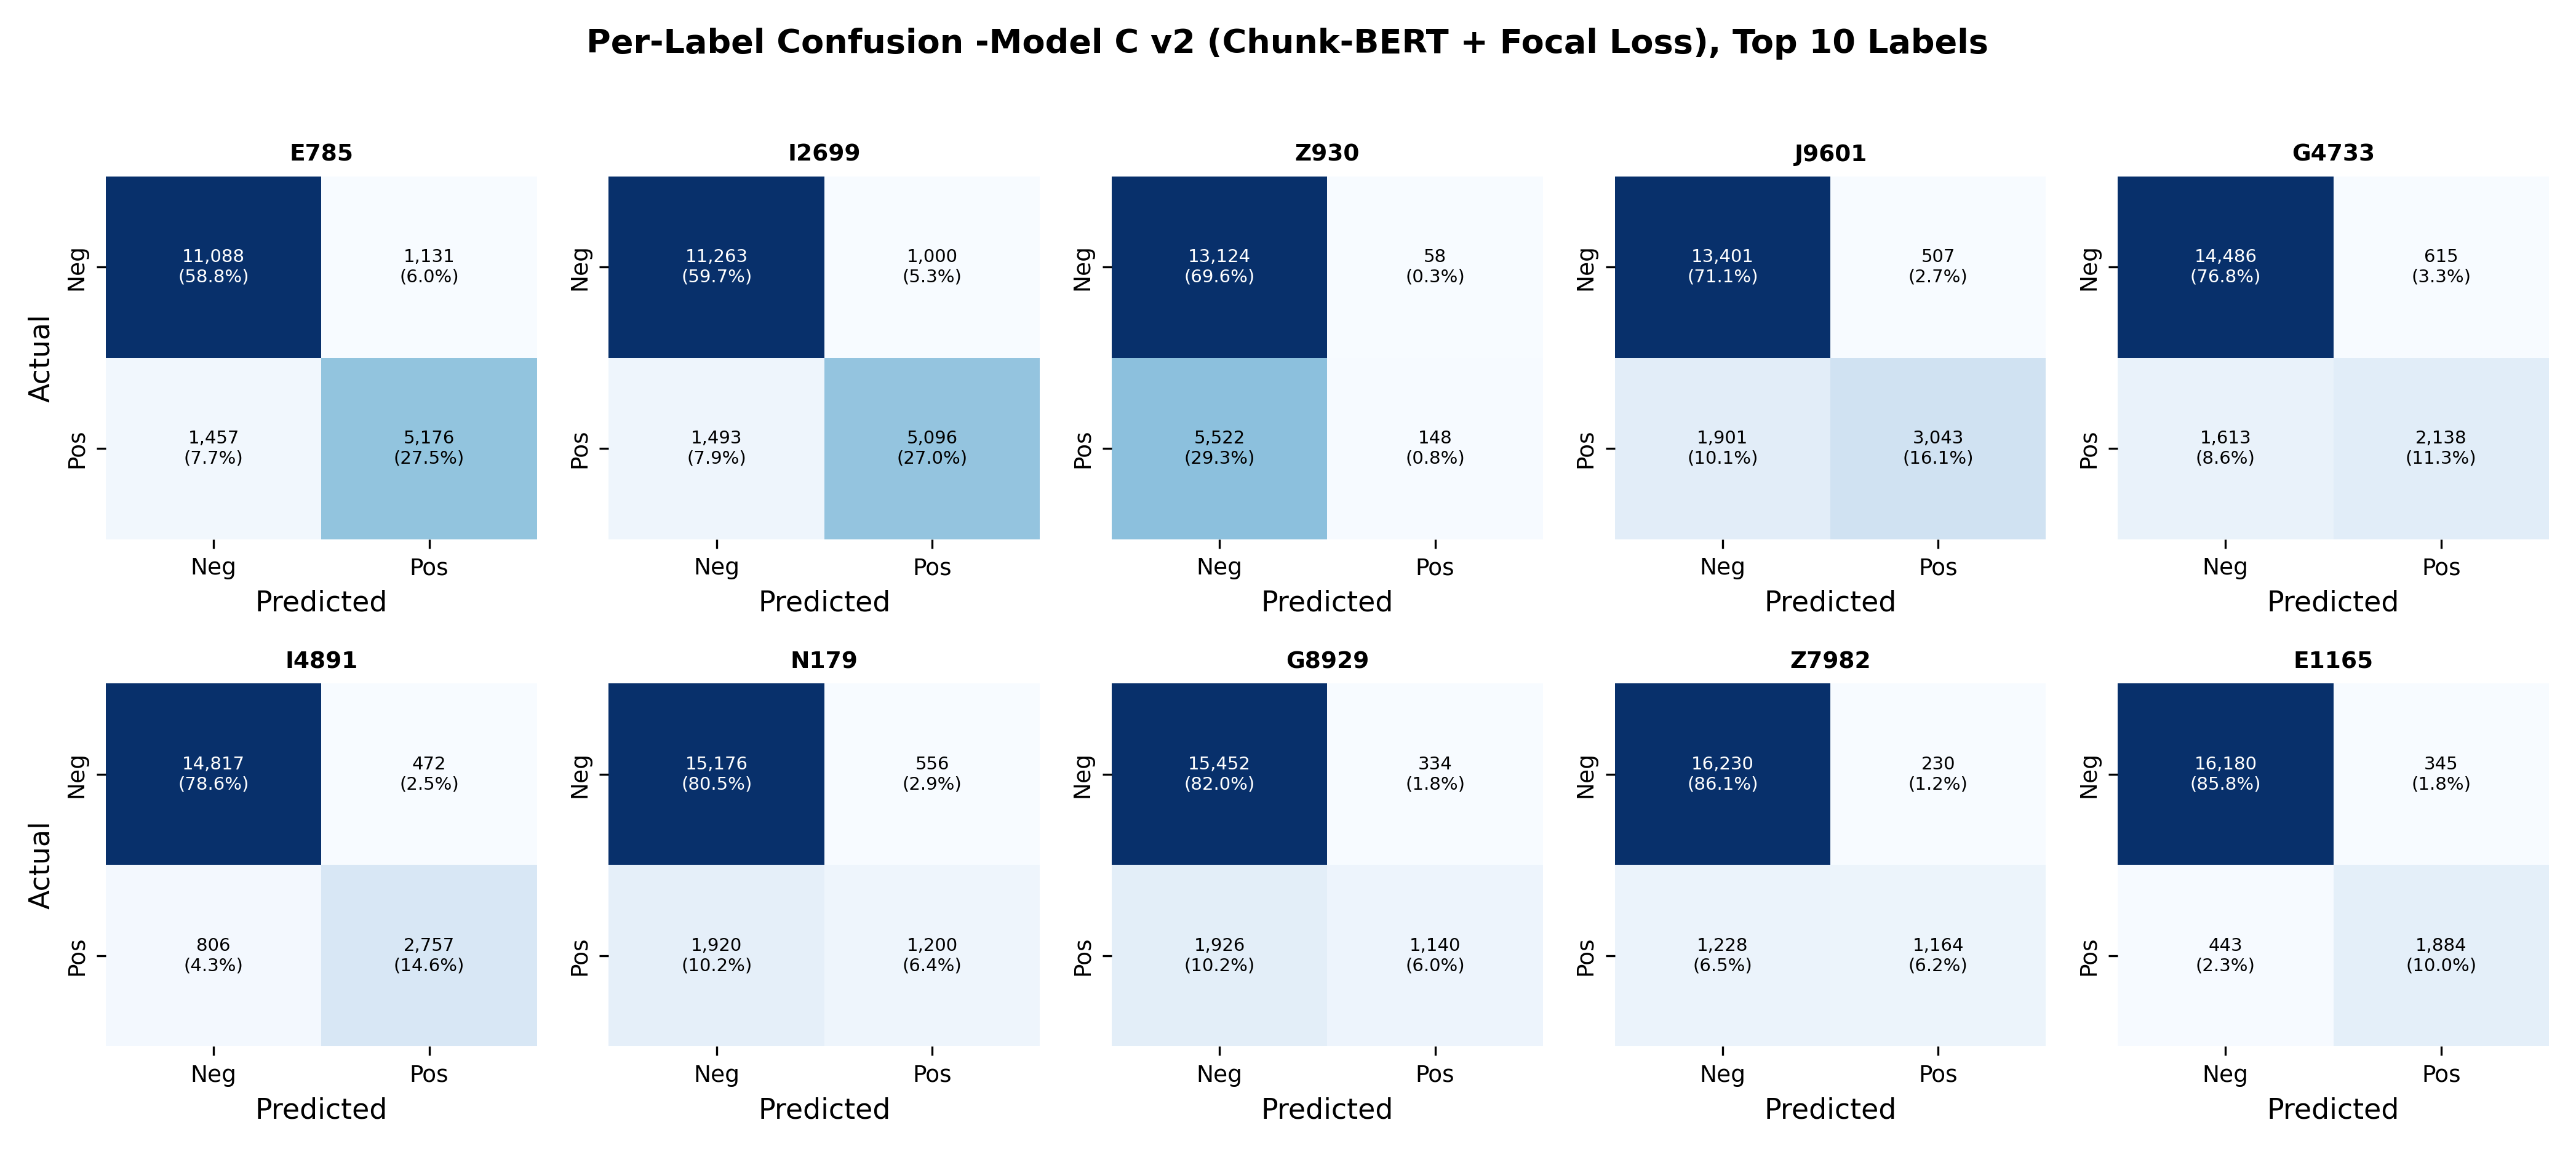
\includegraphics[width=\textwidth]{figures/confusion_matrix_c_v2.png}
    \caption{Per-label confusion matrix for Chunk-BERT v2 (Focal Loss).}
    \label{fig:confusion_v2_ens}
\end{figure}
\vspace{-6pt}
\begin{figure}[H]
    \centering
    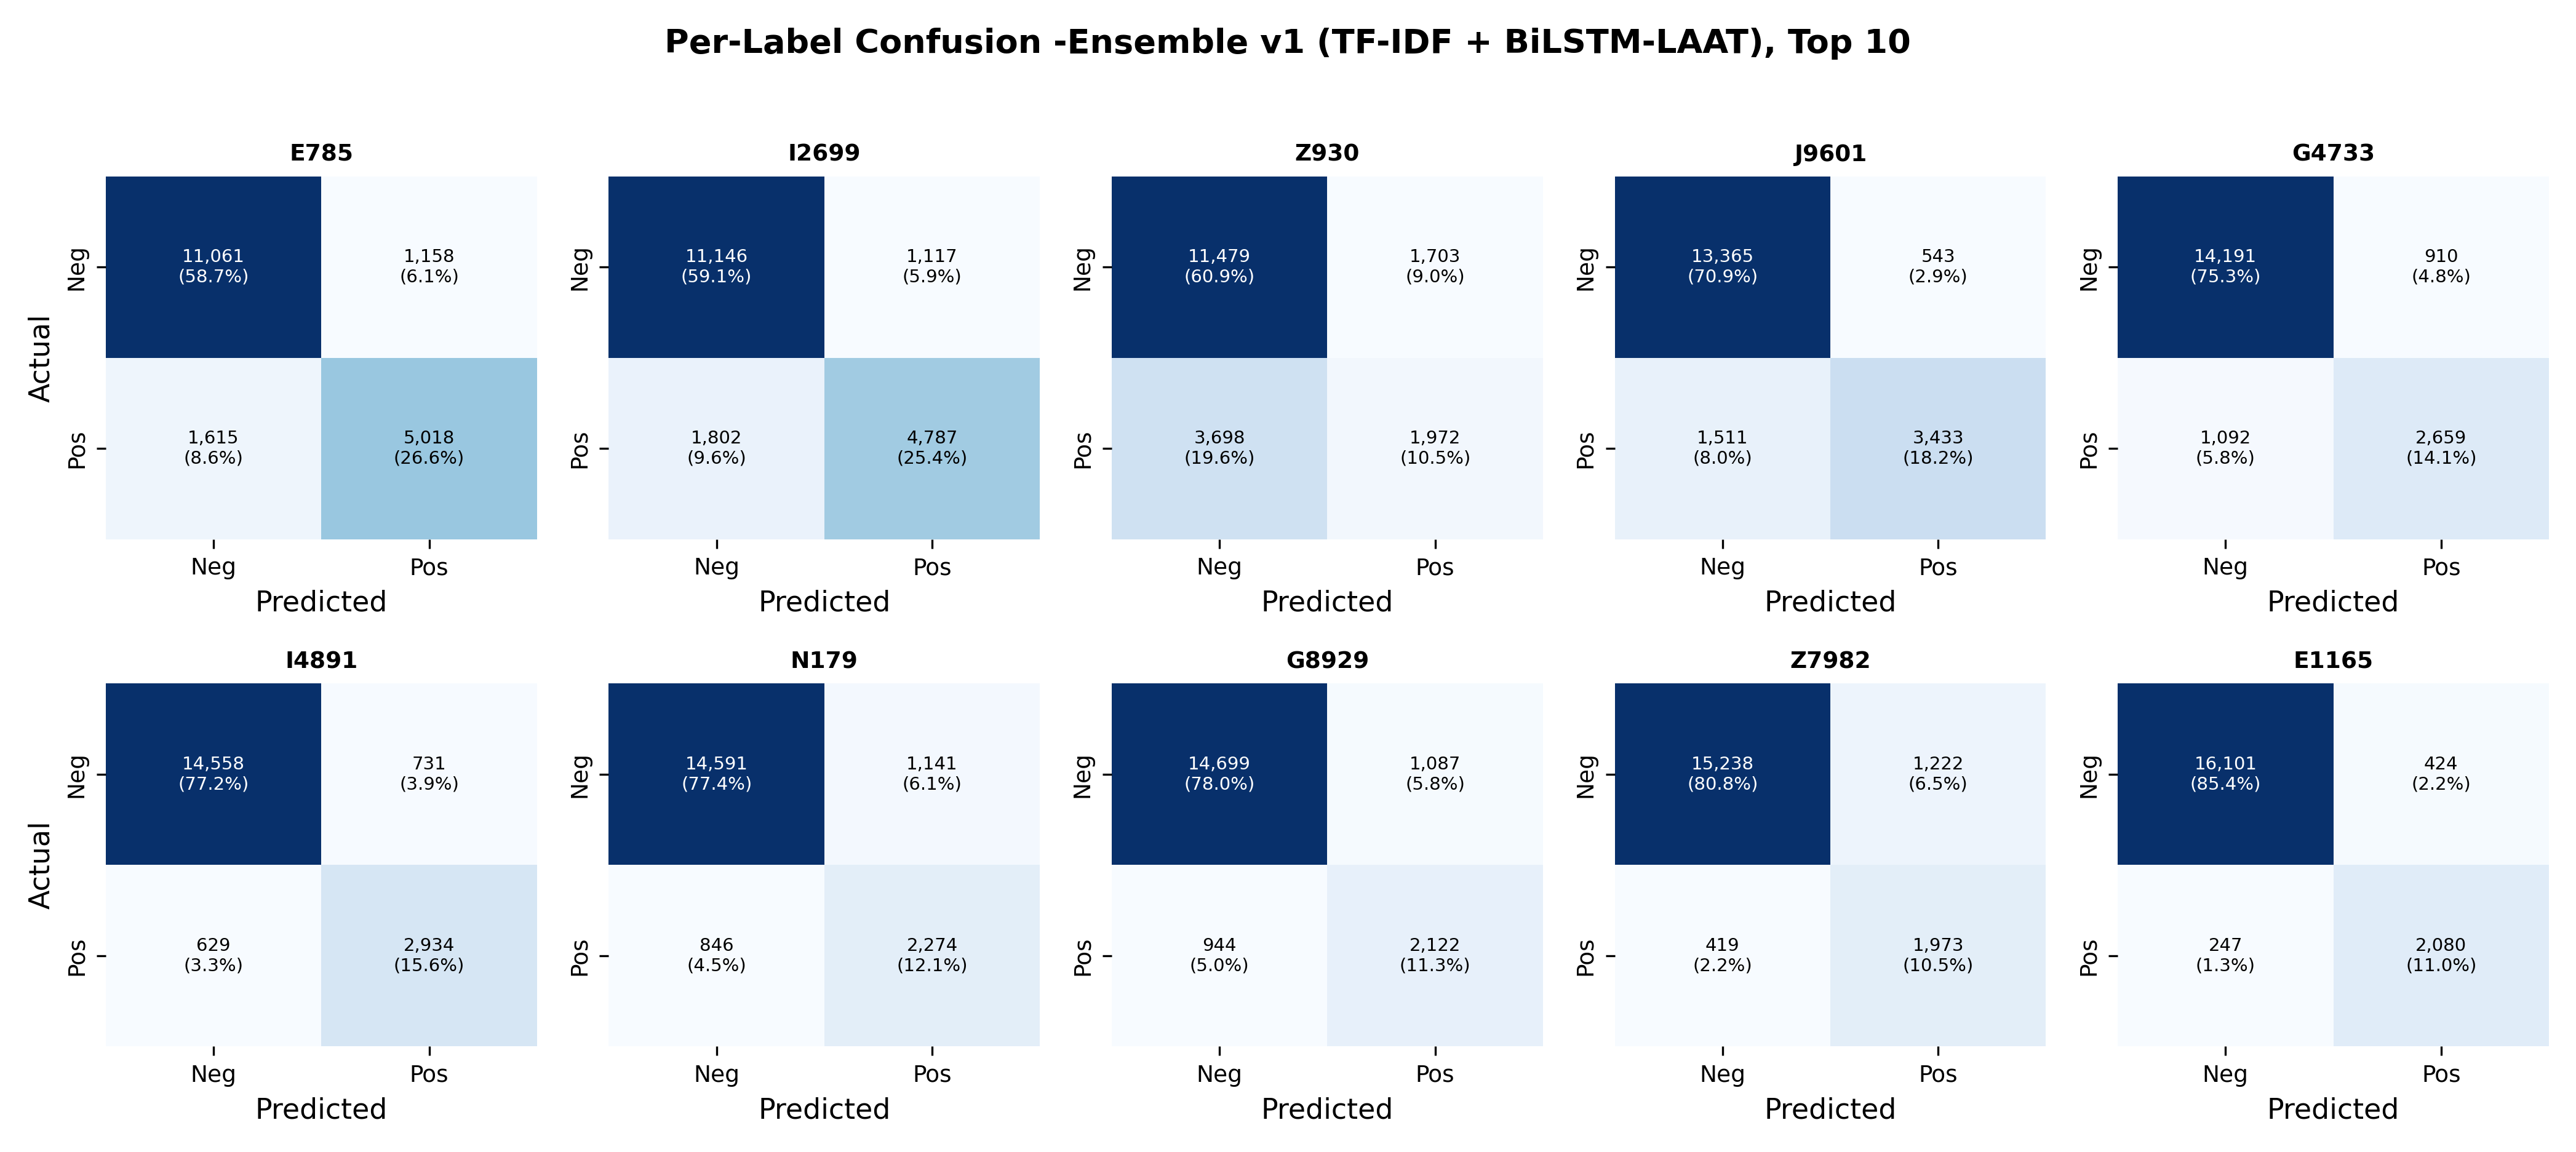
\includegraphics[width=\textwidth]{figures/confusion_matrix_ensemble.png}
    \caption{Per-label confusion matrix for Ensemble v4 (TF-IDF + BiLSTM). Closely matches BiLSTM-LAAT performance.}
    \label{fig:confusion_ens}
\end{figure}

\subsection{Full 50-Label Inter-Code Confusion Heatmaps}

The following $50\times50$ heatmaps show, for each true label, what fraction of its samples were also assigned every other label. Bright off-diagonal spots flag code pairs that a model frequently confuses or co-predicts.

\begin{figure}[H]
    \centering
    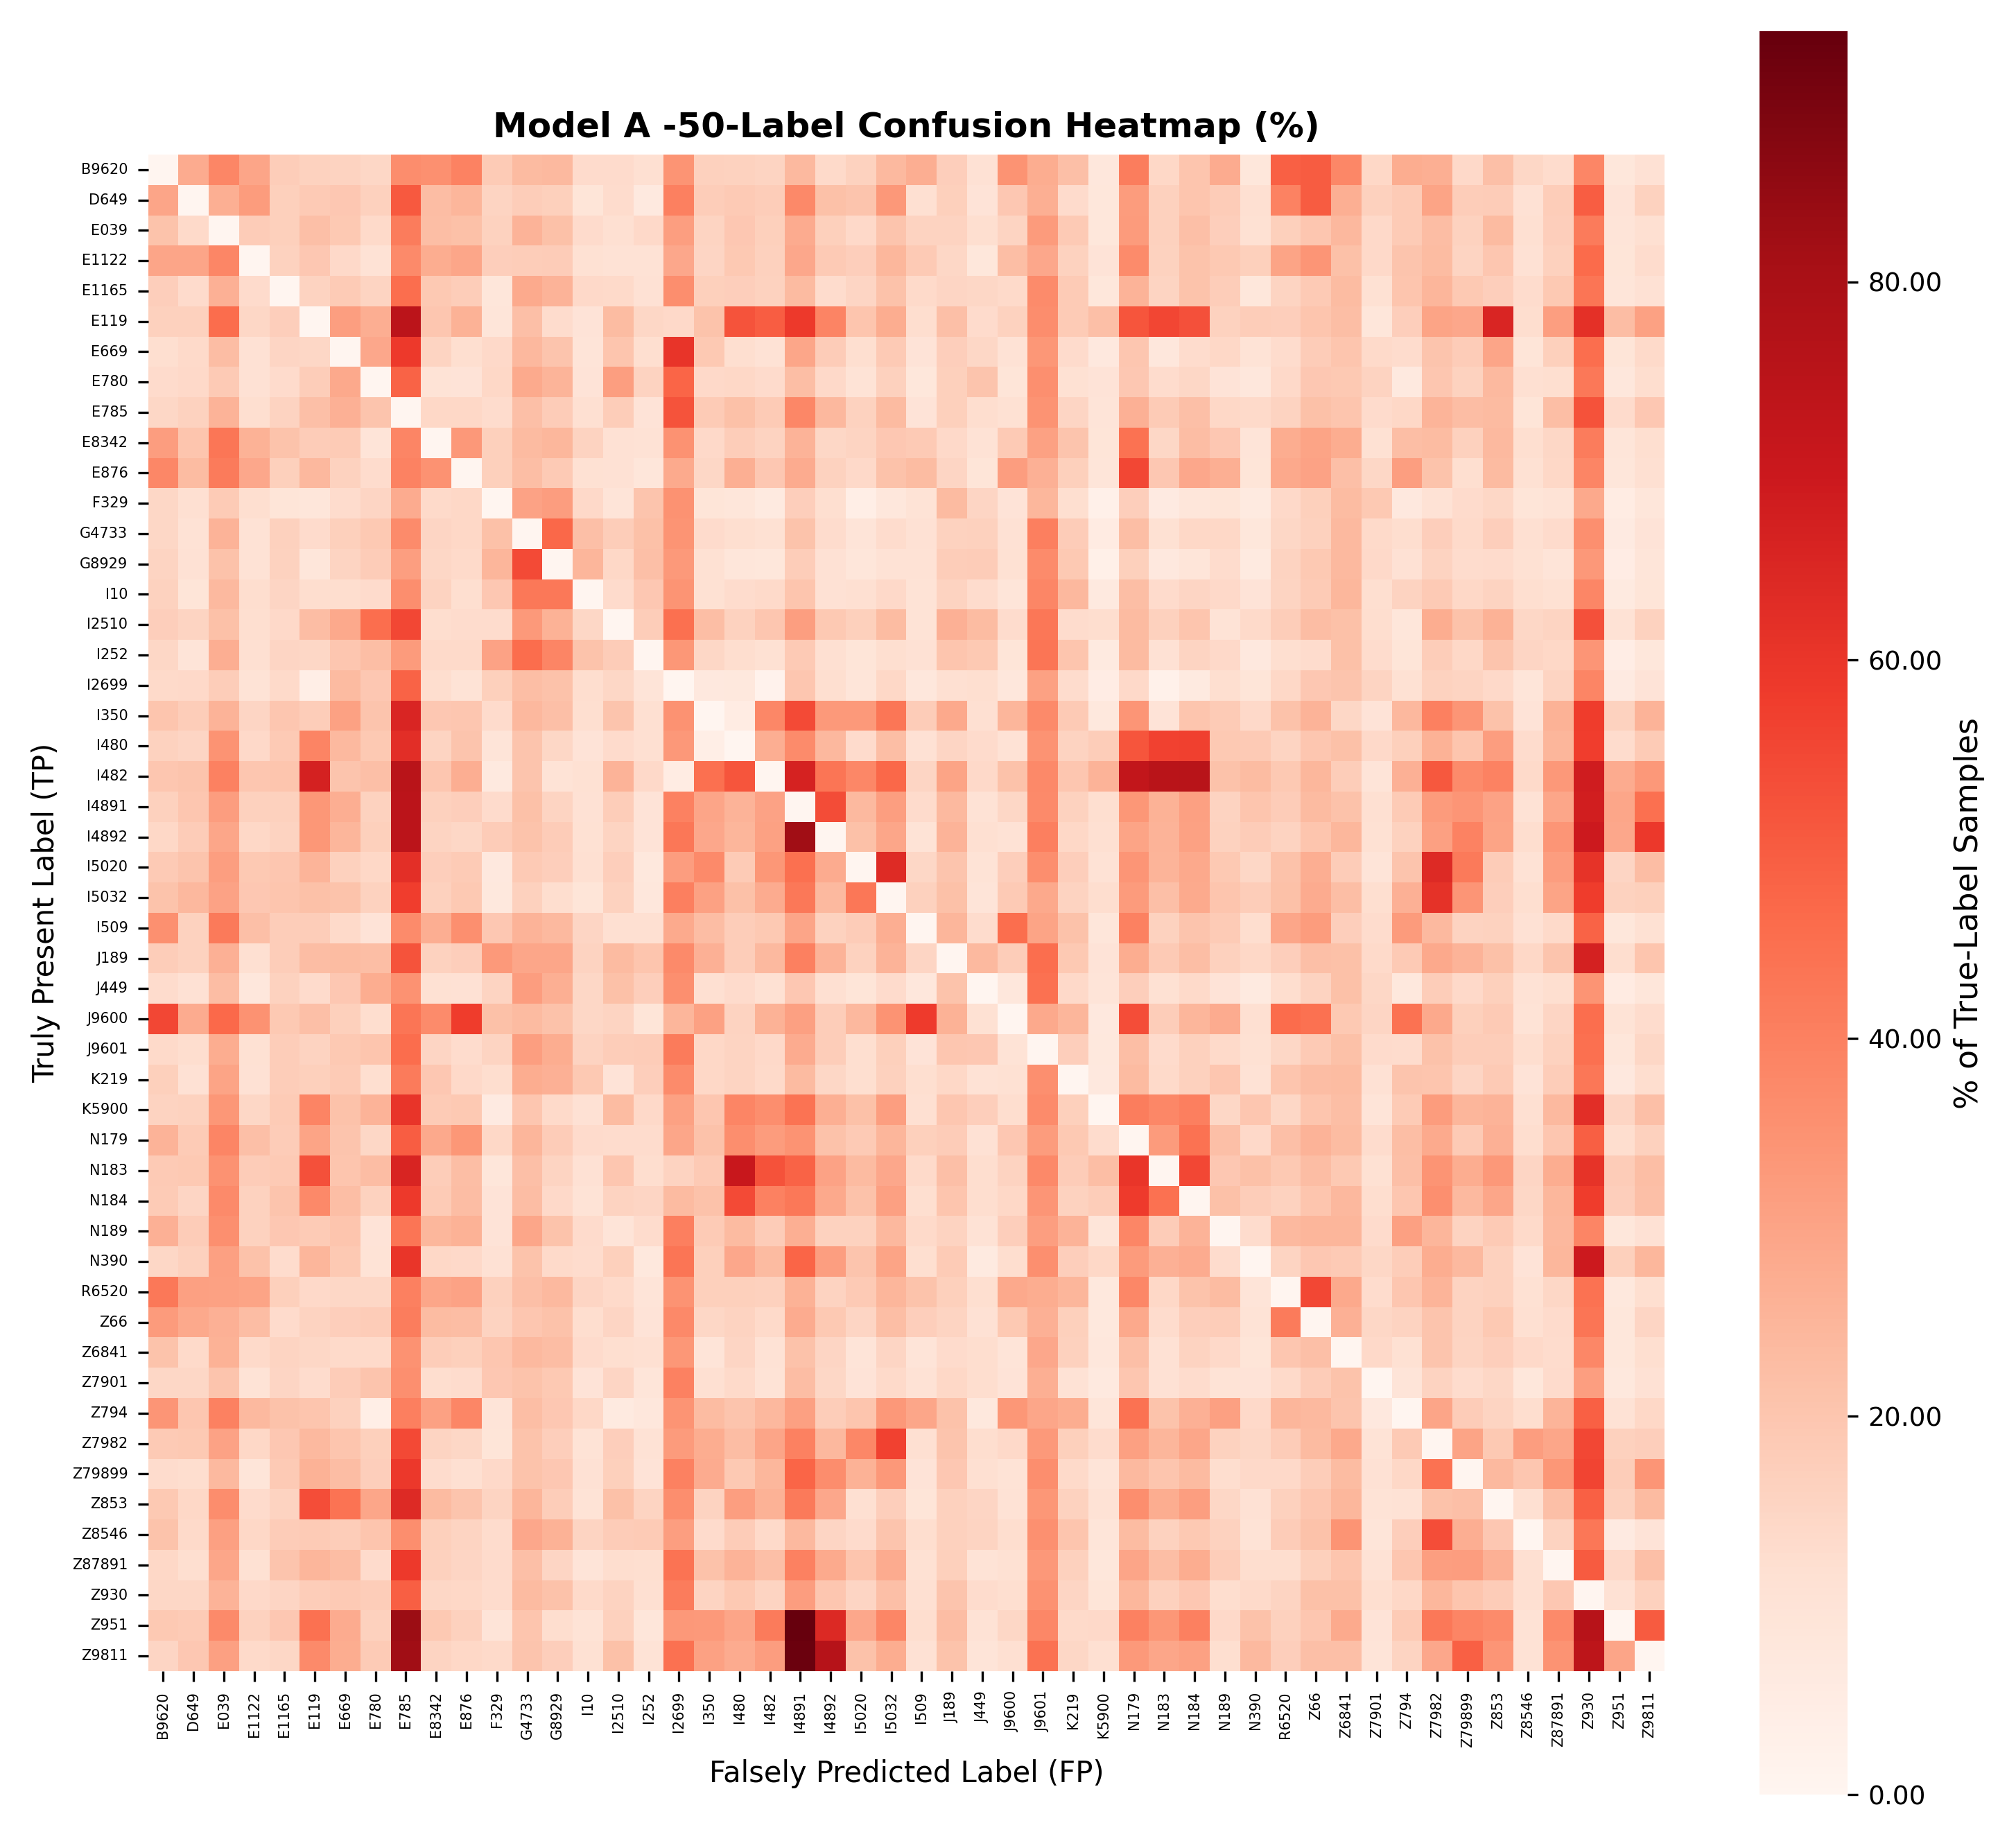
\includegraphics[width=0.65\textwidth]{figures/label_confusion_a.png}
    \caption{Full $50\times50$ inter-label confusion heatmap for TF-IDF + SGD (Model A).}
    \label{fig:label_confusion_base}
\end{figure}
\vspace{-6pt}
\begin{figure}[H]
    \centering
    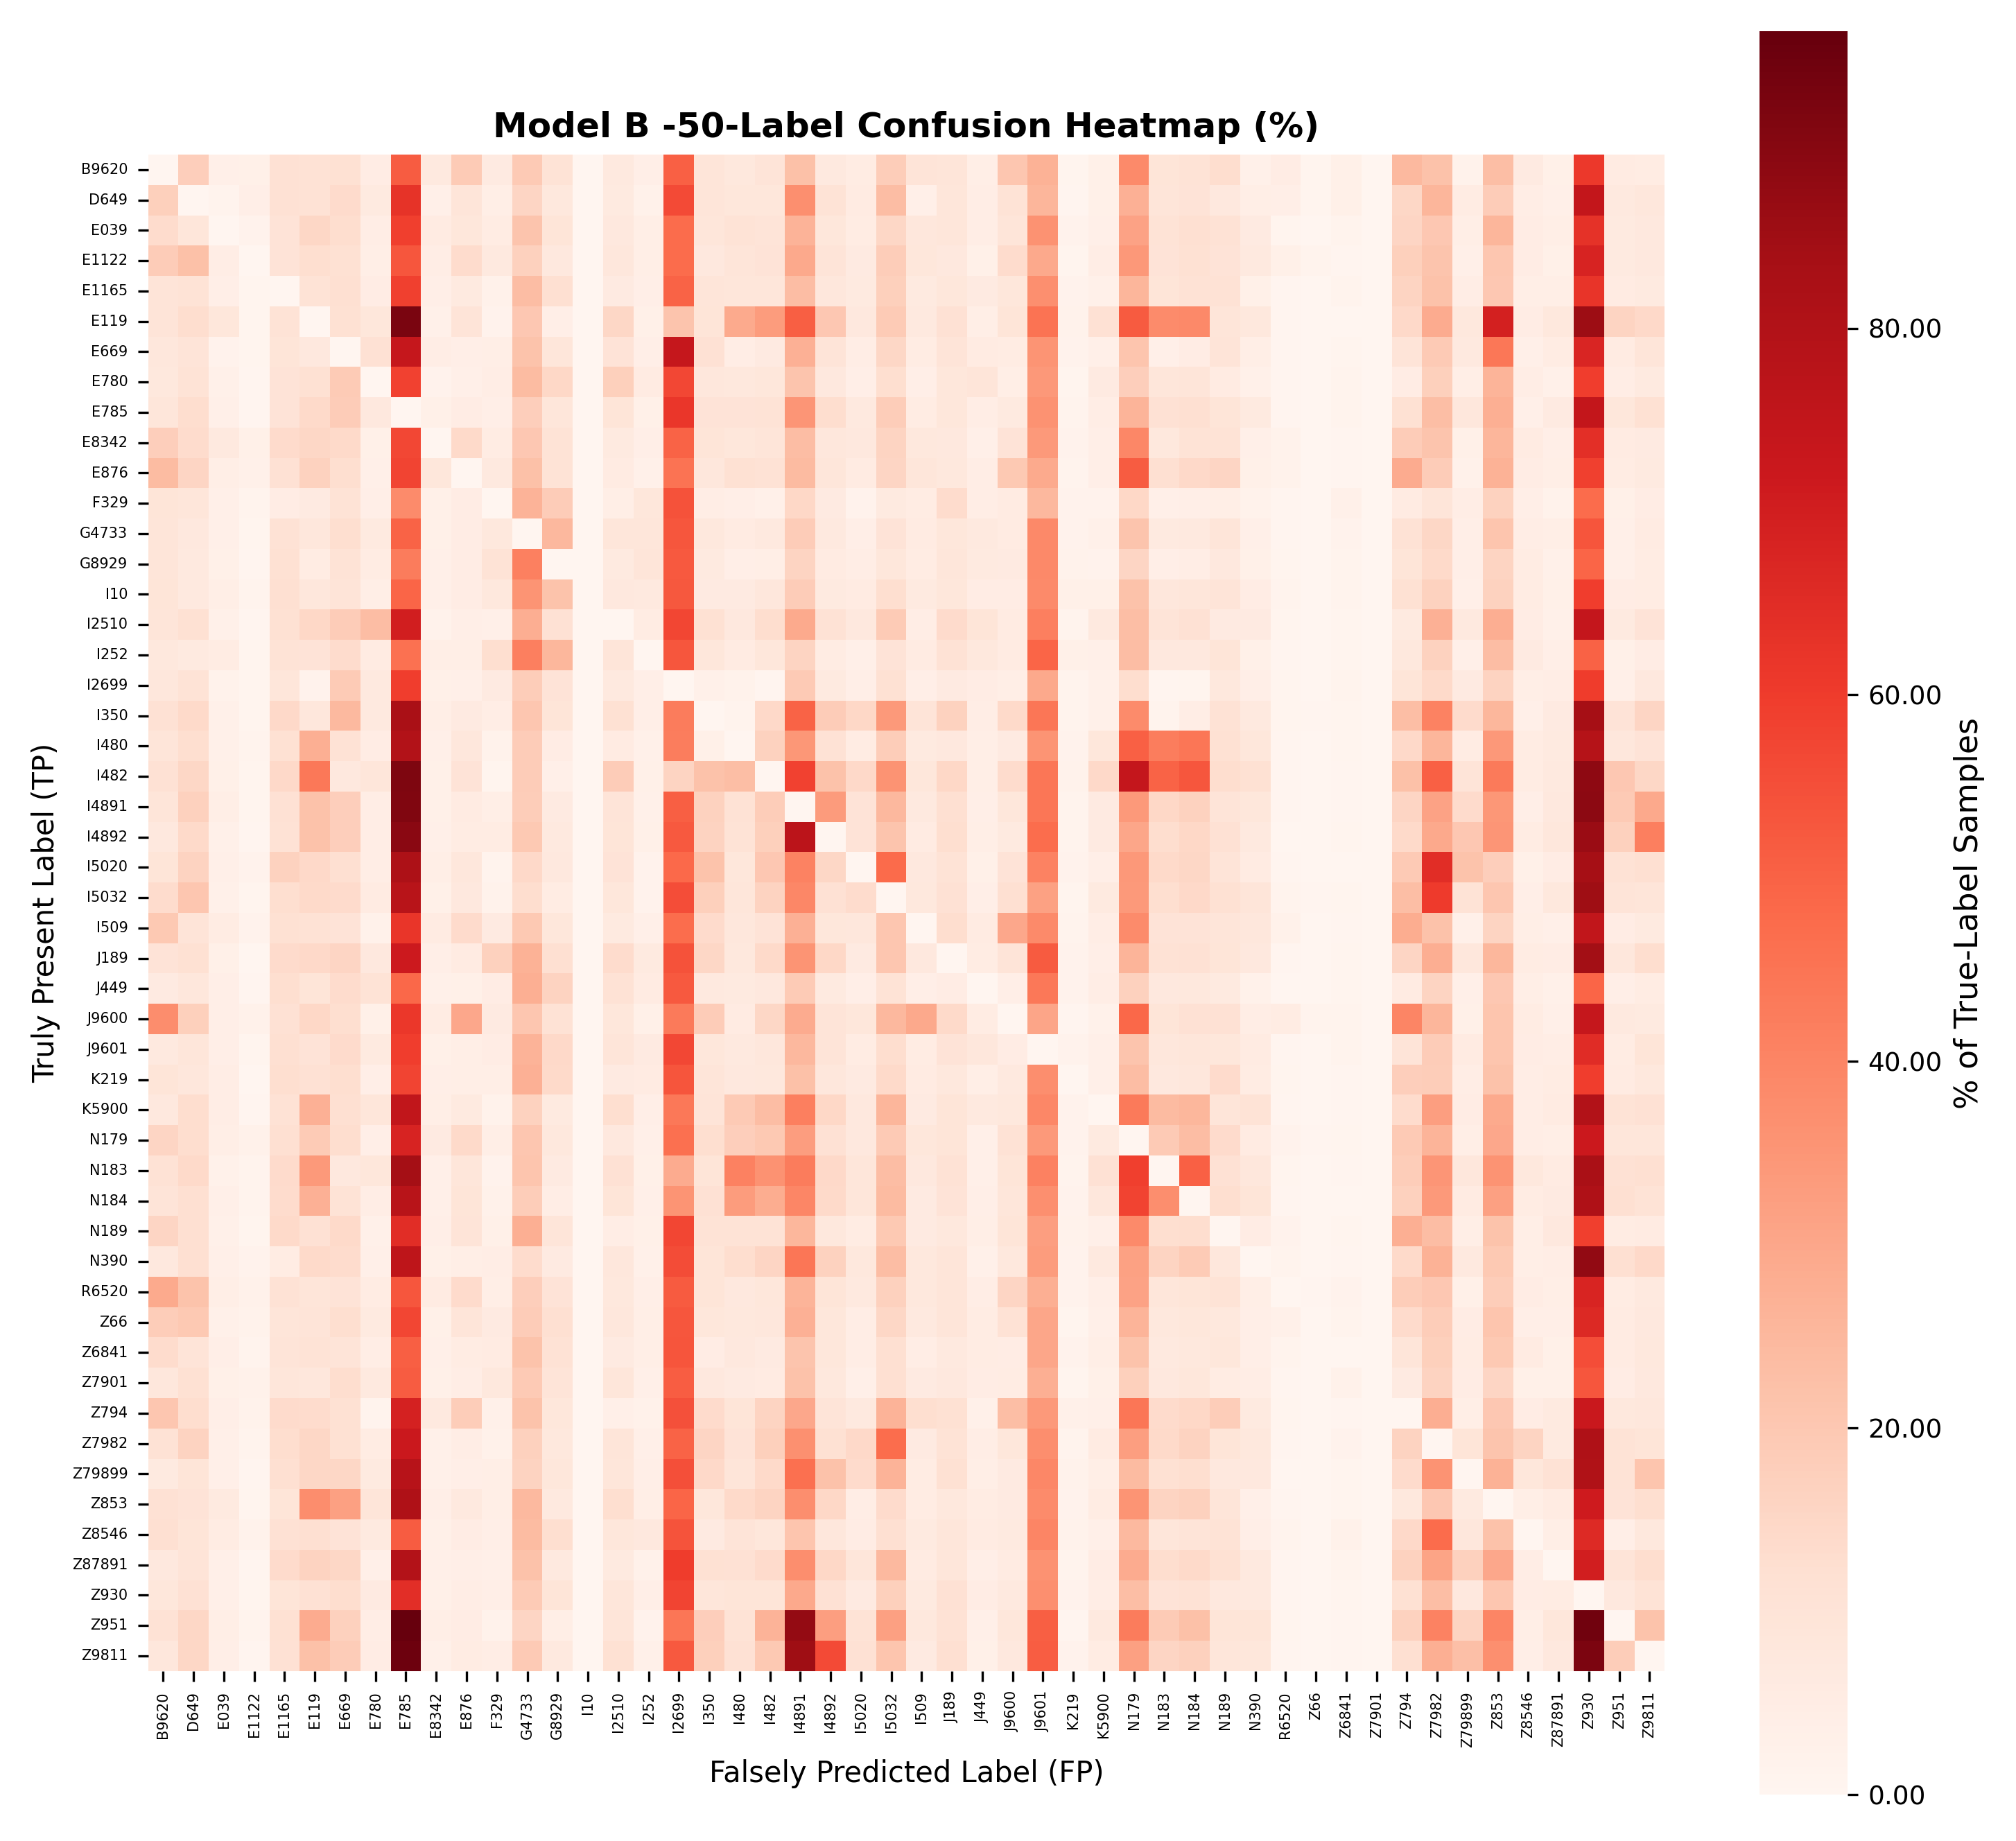
\includegraphics[width=0.65\textwidth]{figures/label_confusion_b.png}
    \caption{$50\times50$ inter-label confusion heatmap for ClinicalBERT (Model B).}
    \label{fig:label_confusion_b}
\end{figure}

\clearpage

\begin{figure}[H]
    \centering
    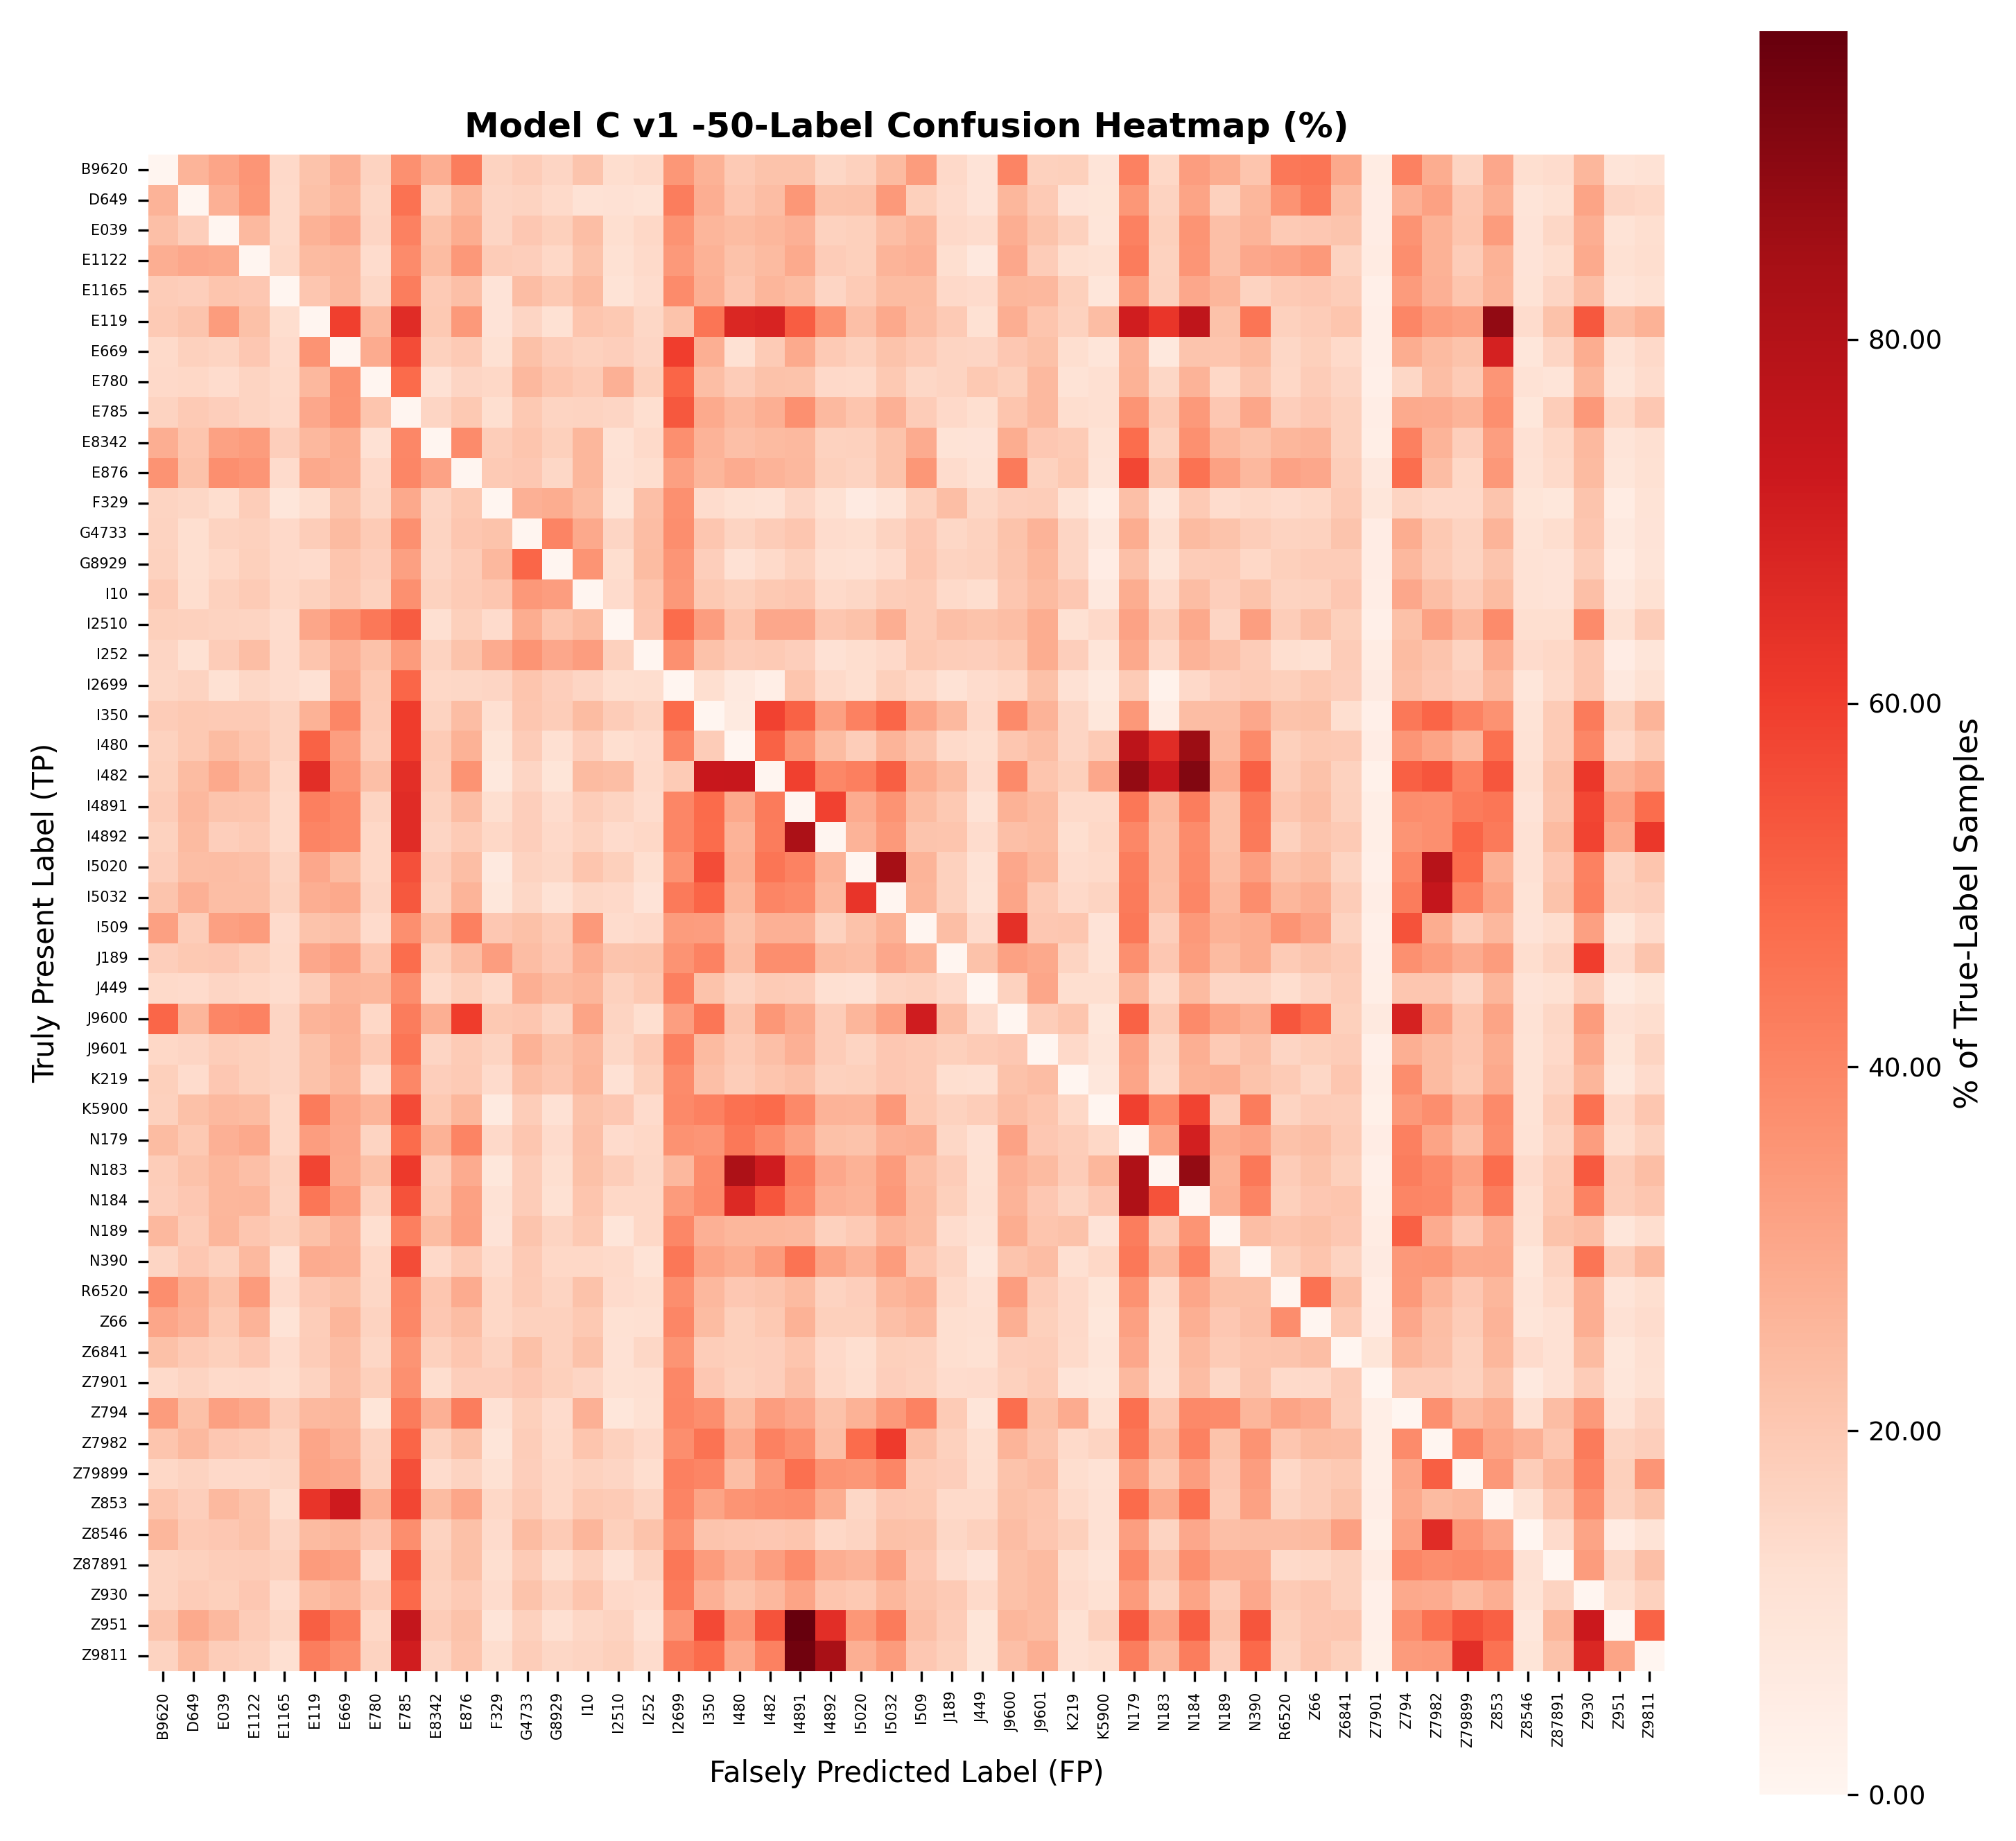
\includegraphics[width=0.65\textwidth]{figures/label_confusion_c.png}
    \caption{$50\times50$ inter-label confusion heatmap for Chunk-BERT v1 (Model C).}
    \label{fig:label_confusion_50}
\end{figure}
\vspace{-6pt}
\begin{figure}[H]
    \centering
    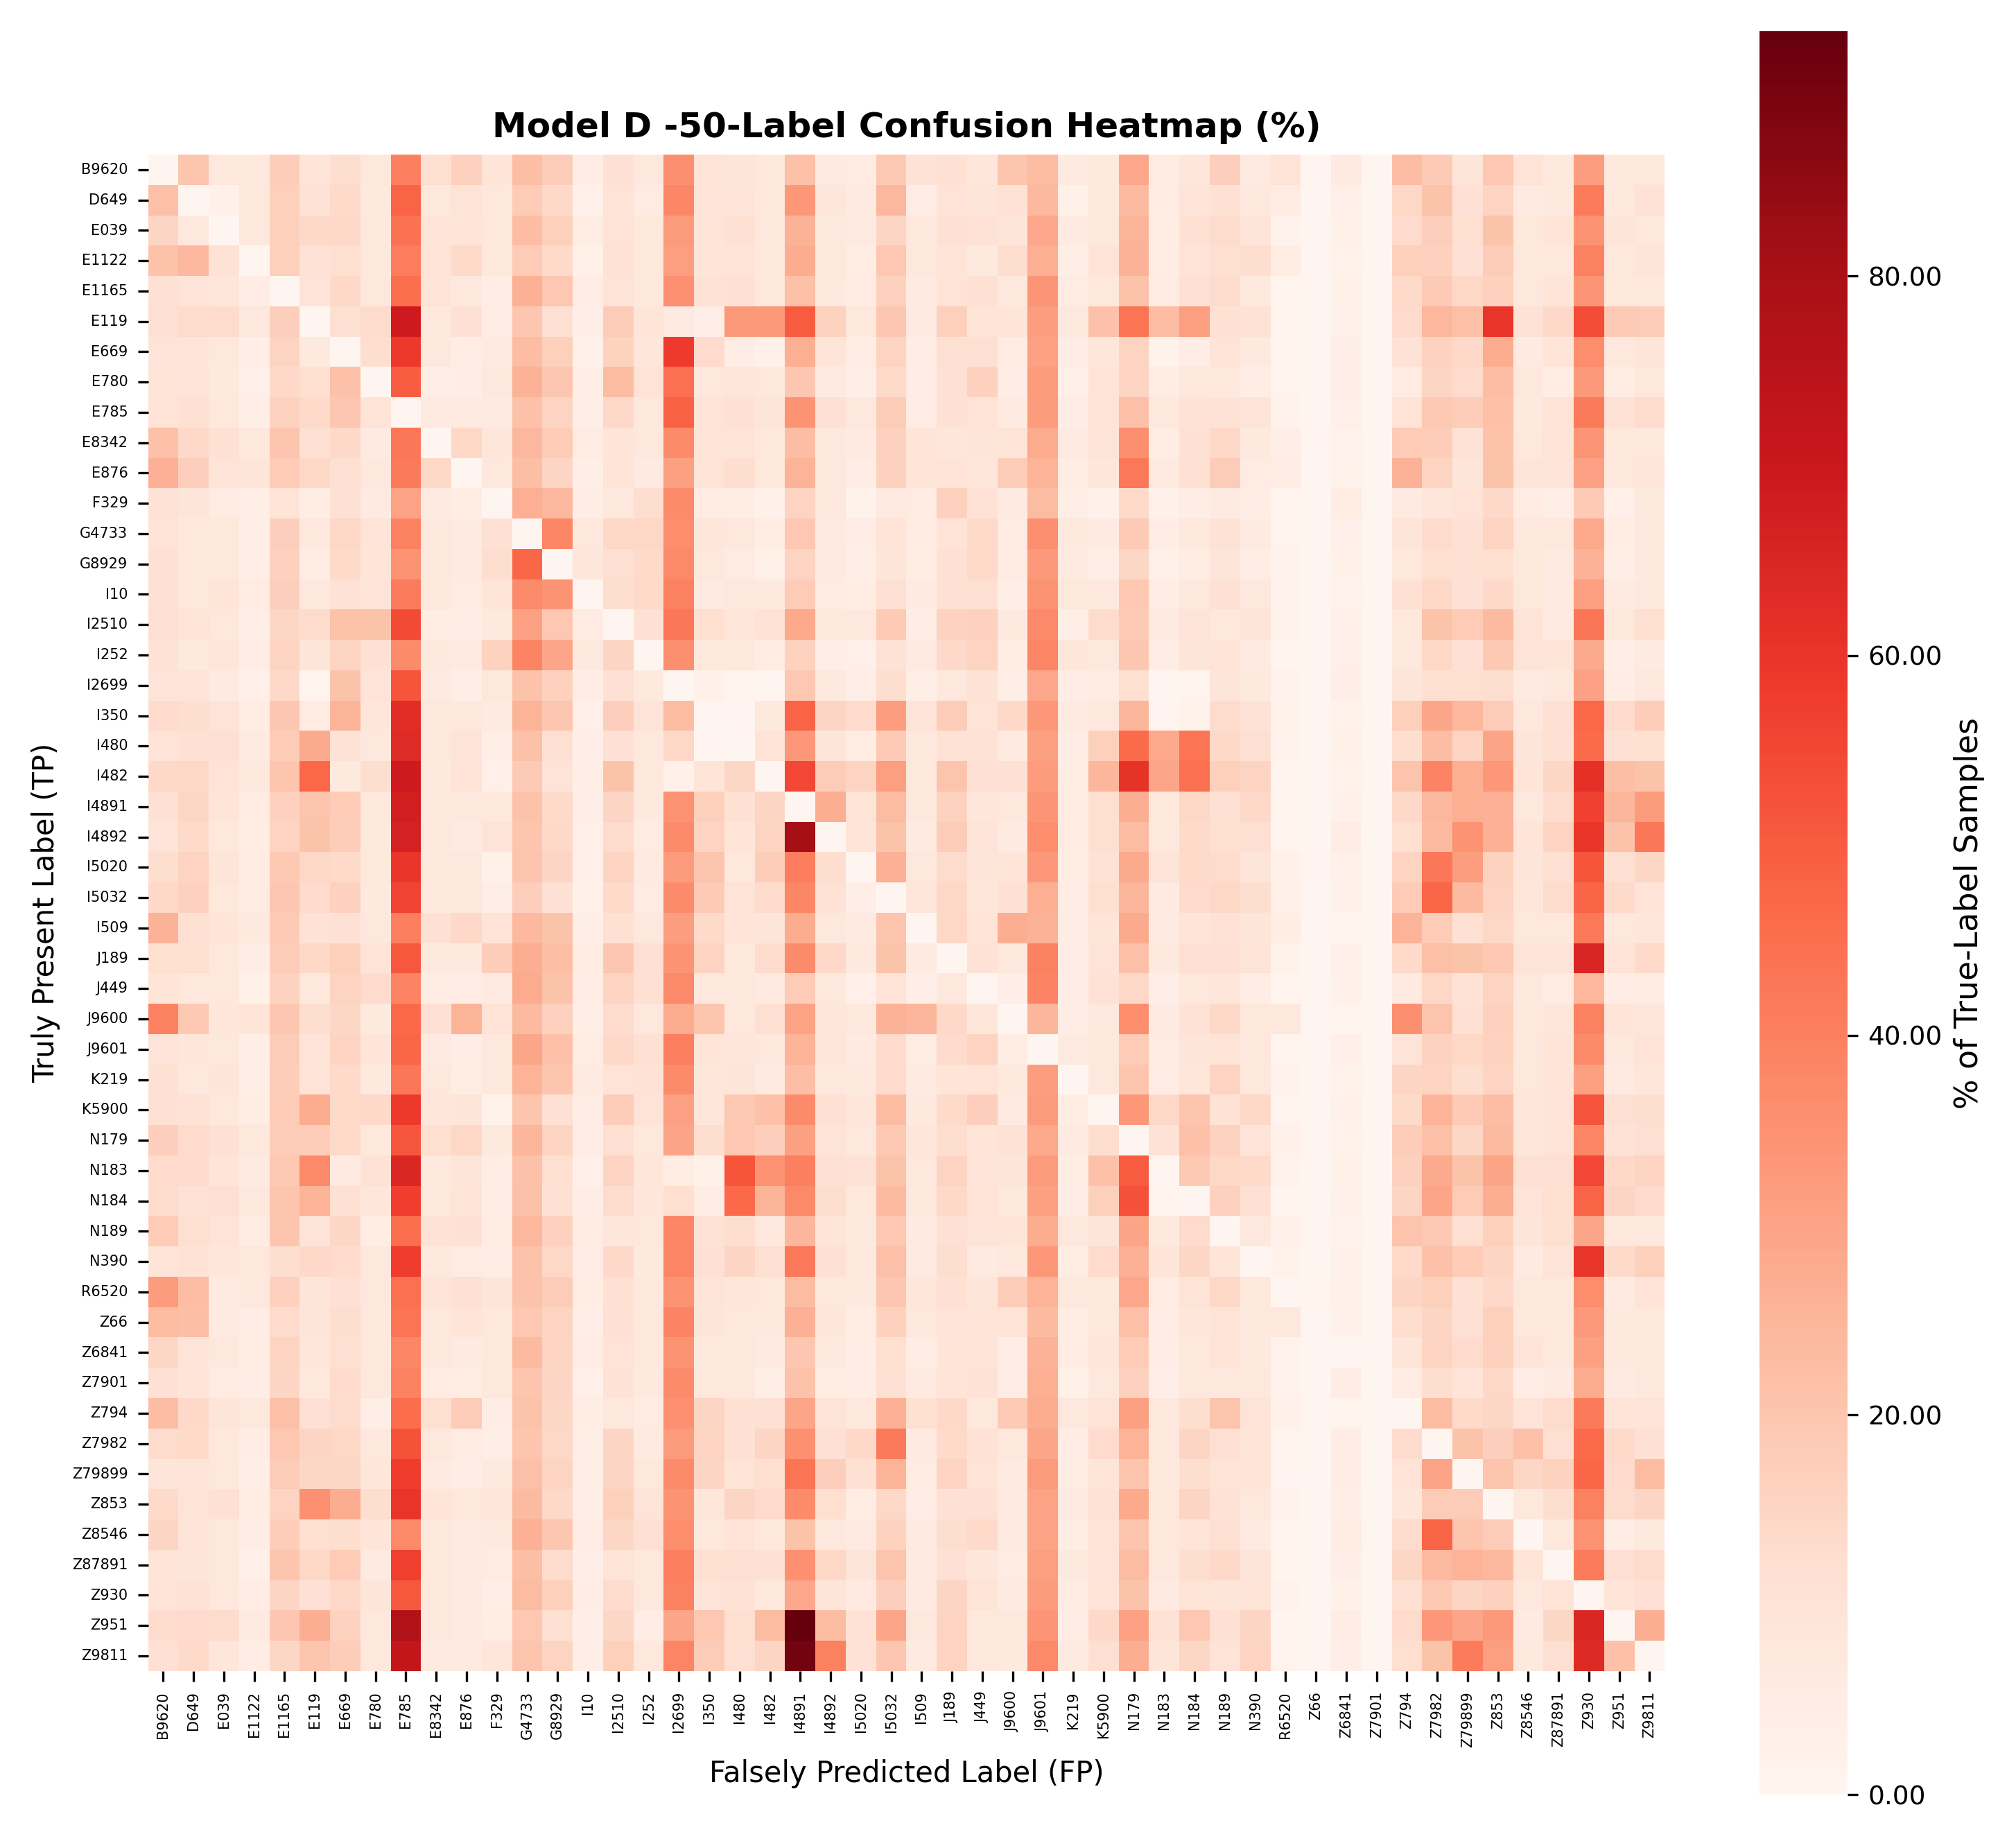
\includegraphics[width=0.65\textwidth]{figures/label_confusion_d.png}
    \caption{$50\times50$ inter-label confusion heatmap for BiLSTM-LAAT (Model D). Notably less off-diagonal confusion.}
    \label{fig:label_confusion_d}
\end{figure}

\clearpage

\begin{figure}[H]
    \centering
    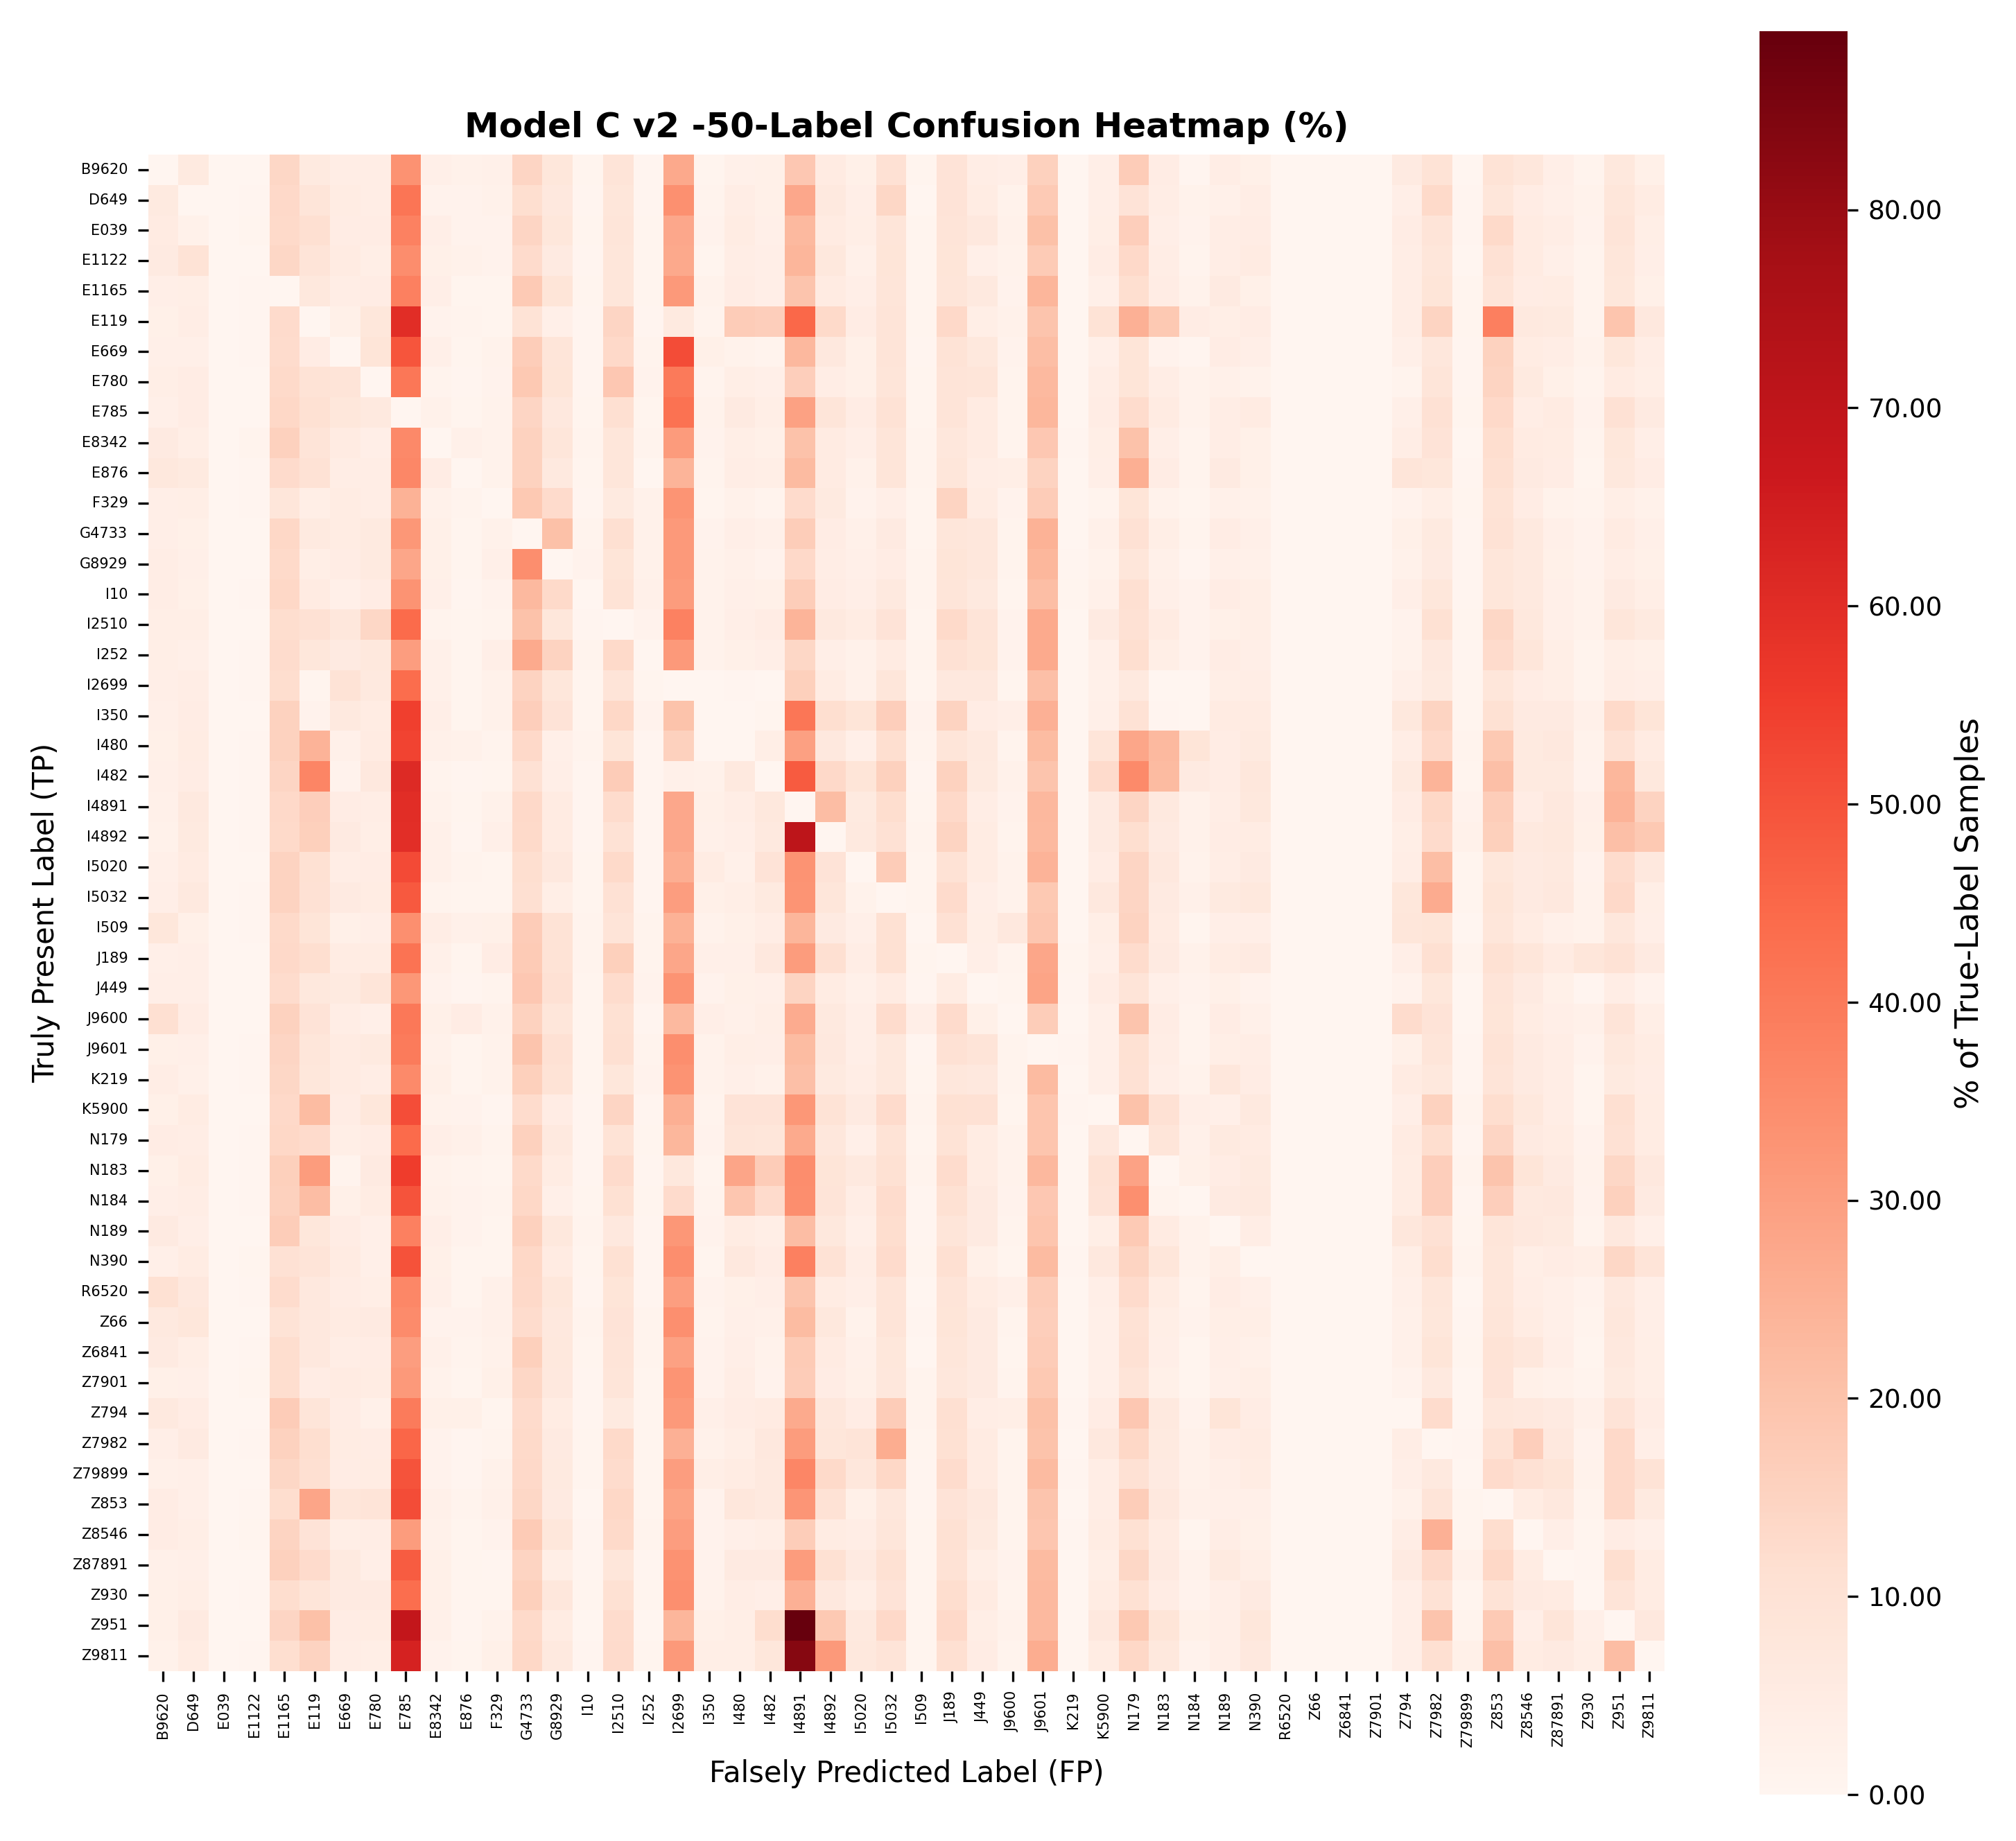
\includegraphics[width=0.65\textwidth]{figures/label_confusion_c_v2.png}
    \caption{$50\times50$ inter-label confusion heatmap for Chunk-BERT v2 (Focal Loss).}
    \label{fig:label_confusion_50_2}
\end{figure}
\vspace{-6pt}
\begin{figure}[H]
    \centering
    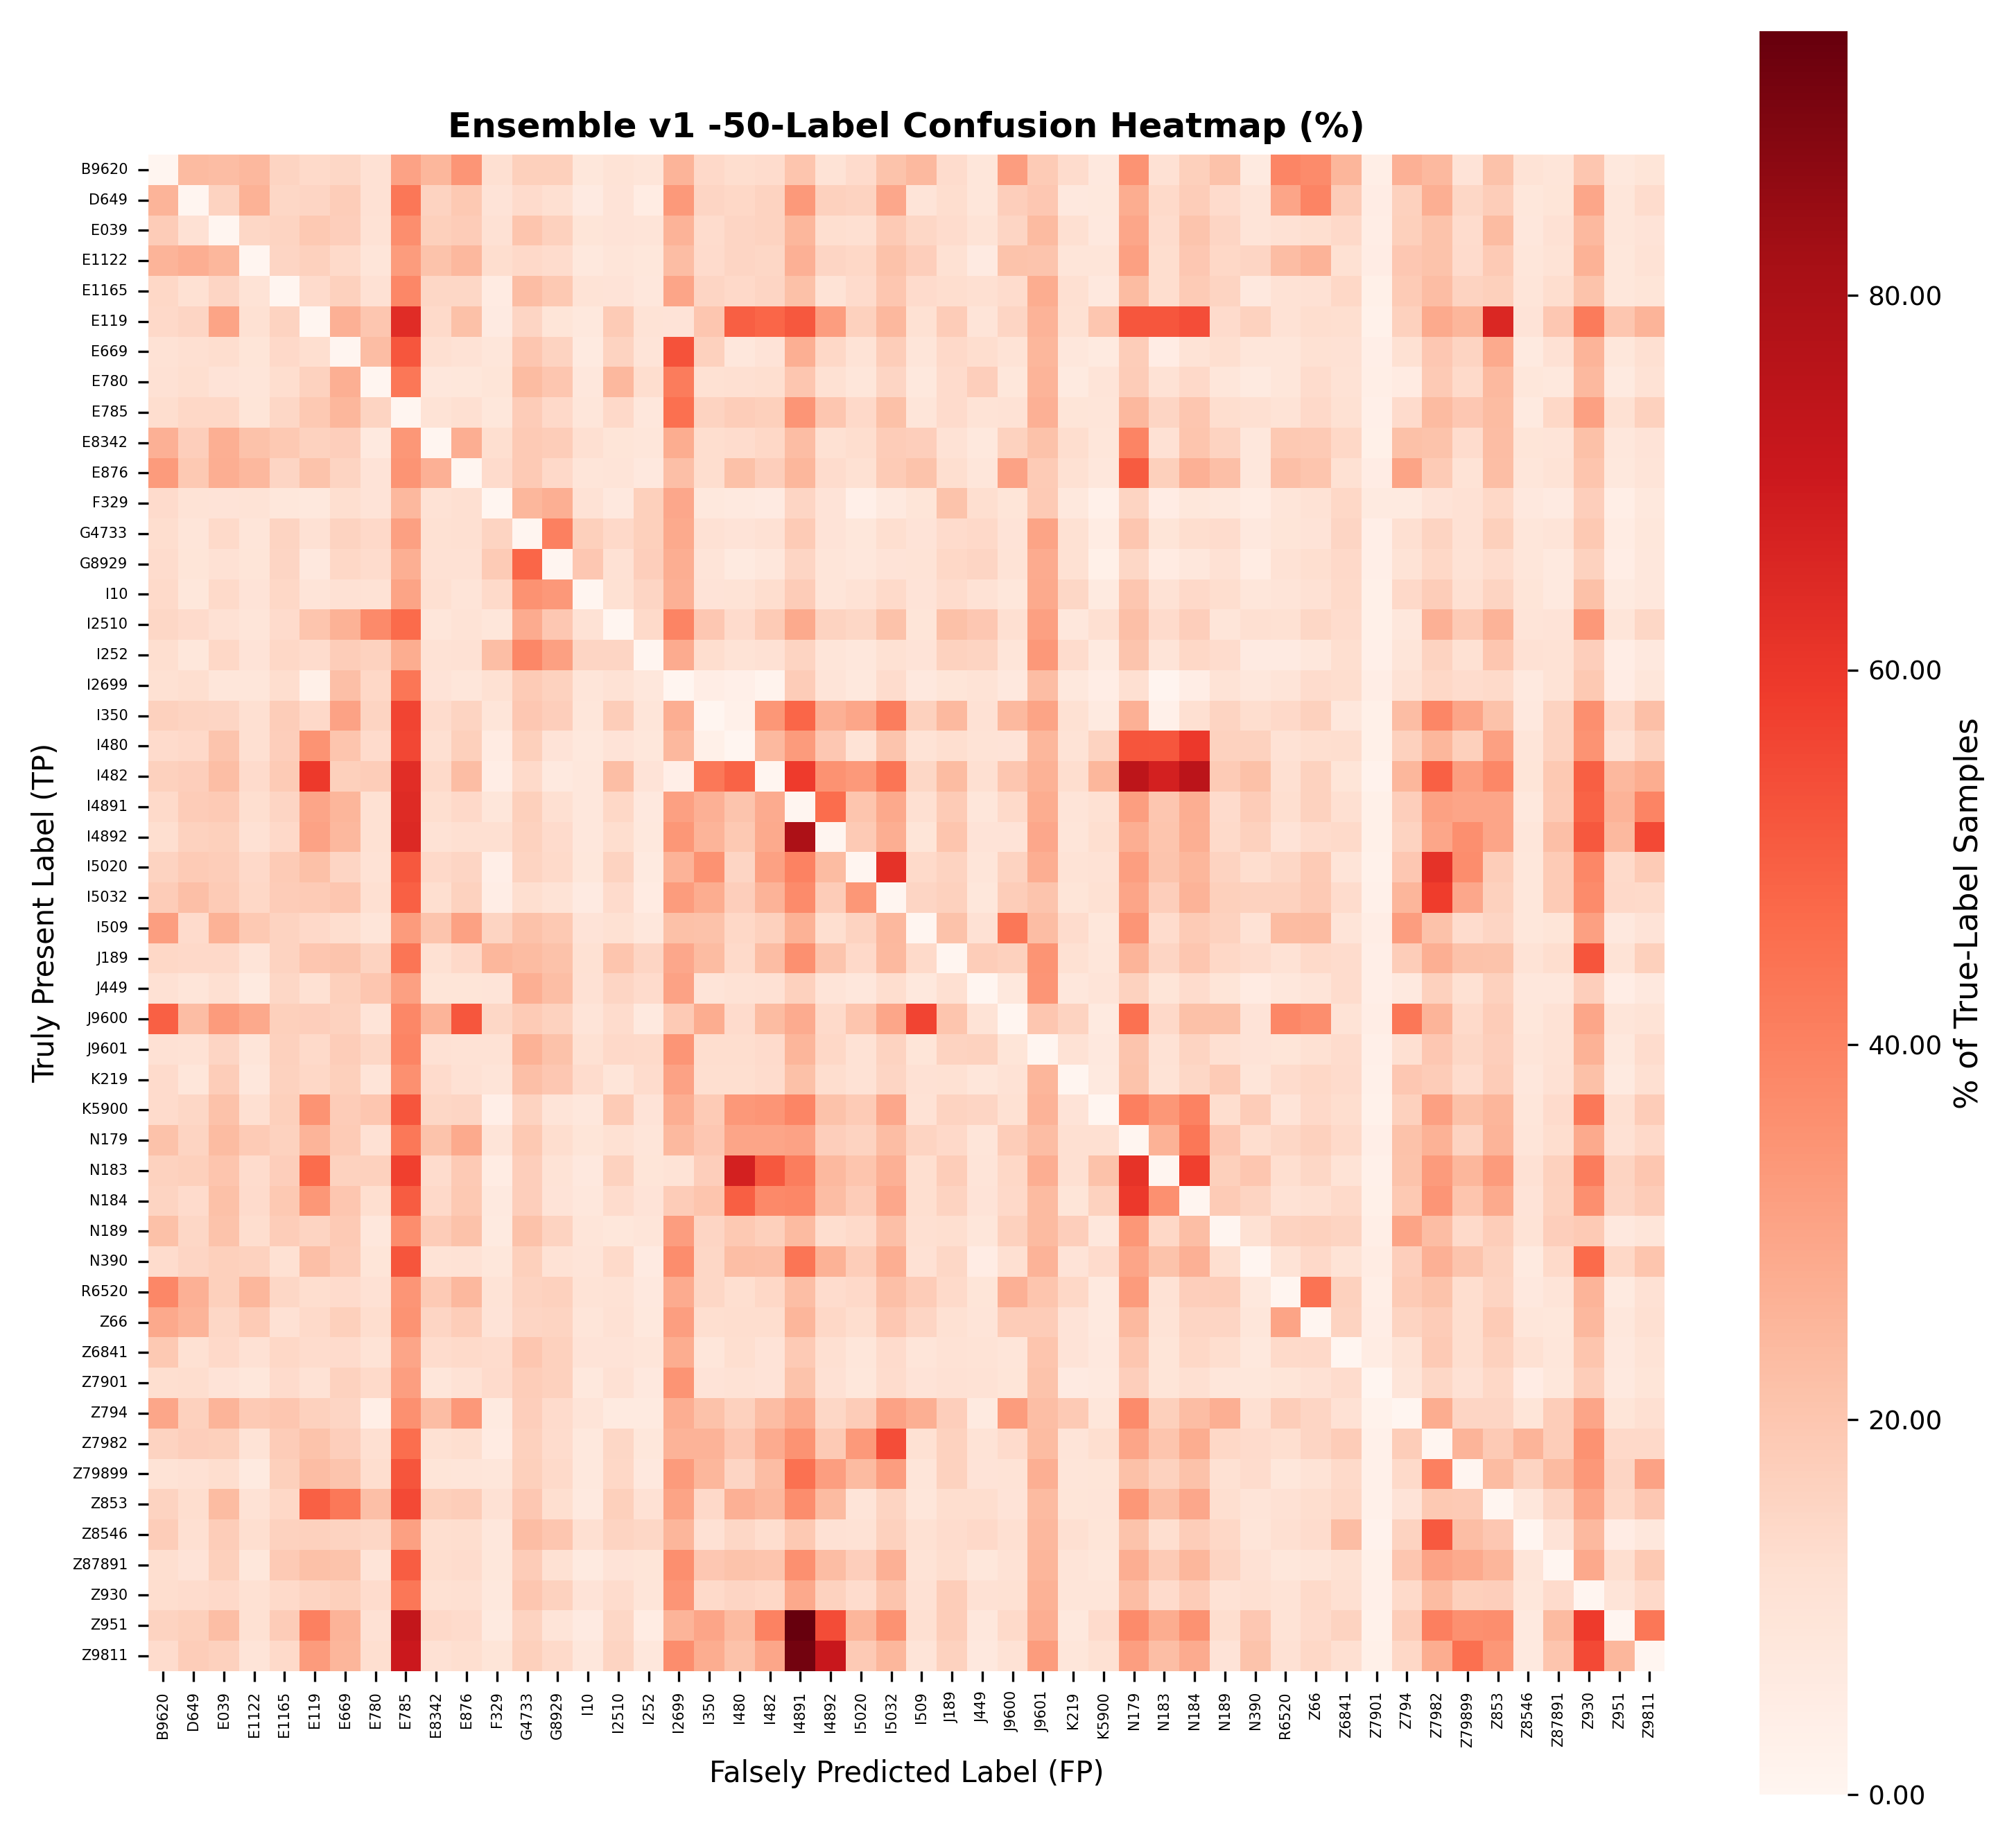
\includegraphics[width=0.65\textwidth]{figures/label_confusion_ensemble.png}
    \caption{$50\times50$ inter-label confusion heatmap for Ensemble v4 (TF-IDF + BiLSTM). Cleanest diagonal pattern.}
    \label{fig:label_confusion_ens}
\end{figure}

\subsection{Most Confused Label Pairs}
\label{sec:confused_pairs}

\begin{table}[H]
\centering
\caption{Top-5 most confused label pairs per model (bidirectional swap count on test set).}
\label{tab:confused_pairs}
\footnotesize
\resizebox{\textwidth}{!}{%
\begin{tabular}{l l l r l}
\toprule
\textbf{Model} & \textbf{Code A} & \textbf{Code B} & \textbf{Swaps} & \textbf{Clinical Interpretation} \\
\midrule
TF-IDF+SGD & Z6841 (BMI 40+)       & Z930 (Tracheostomy)     & 609 & Unrelated administrative codes \\
            & E039 (Hypothyroid)     & Z930 (Tracheostomy)     & 597 & Unrelated; high FP for Z930 \\
            & F329 (Depression)      & Z930 (Tracheostomy)     & 594 & Z930 over-predicted \\
            & I2699 (Heart dis.)     & Z930 (Tracheostomy)     & 504 & Z930 dominates errors \\
            & Z66 (DNR)              & Z930 (Tracheostomy)     & 462 & Administrative code confusion \\
\midrule
Chunk-BERT  & Z7901 (Anticoag.)      & Z930 (Tracheostomy)     & 1,108 & Worst pair; administrative \\
            & I10 (Hypertension)     & J9601 (Resp. failure)   & 781 & Common comorbidity pair \\
            & I10 (Hypertension)     & Z930 (Tracheostomy)     & 763 & High FP for Z930 \\
            & E039 (Hypothyroid)     & Z930 (Tracheostomy)     & 756 & Same Z930 pattern \\
            & F329 (Depression)      & Z930 (Tracheostomy)     & 756 & Same Z930 pattern \\
\midrule
BiLSTM-LAAT & F329 (Depression)      & Z930 (Tracheostomy)     & 489 & Reduced vs.\ Chunk-BERT \\
            & E785 (Hyperlipid.)     & Z930 (Tracheostomy)     & 382 & Still Z930-driven \\
            & I2699 (Heart dis.)     & I350 (Aortic stenosis)  & 375 & \textit{Clinically related} \\
            & I2699 (Heart dis.)     & Z930 (Tracheostomy)     & 378 & Mixed clinical/admin \\
            & I5020 (Systolic HF)    & I5032 (Diastolic HF)    & 326 & \textit{Closely related subtypes} \\
\midrule
Ensemble v4 & F329 (Depression)      & Z930 (Tracheostomy)     & 436 & Slightly improved vs.\ BiLSTM \\
            & E785 (Hyperlipid.)     & Z930 (Tracheostomy)     & 380 & Persistent Z930 issue \\
            & I2699 (Heart dis.)     & I350 (Aortic stenosis)  & 358 & \textit{Clinically related} \\
            & I2699 (Heart dis.)     & Z930 (Tracheostomy)     & 364 & Mixed \\
            & I5020 (Systolic HF)    & I5032 (Diastolic HF)    & 313 & \textit{HF subtype confusion} \\
\bottomrule
\end{tabular}}
\end{table}

One code dominates the confusion tables: Z930 (tracheostomy status). It shows up as a top confusion partner for every model, largely because tracheostomy patients tend to have many concurrent diagnoses, making the code easy to over-predict. BiLSTM-LAAT cuts Z930-related swaps by 40 to 70\% compared to Chunk-BERT v1, and its remaining top confusions shift toward clinically related pairs like I5020/I5032 (systolic vs.\ diastolic heart failure) and I2699/I350 (heart disease subtypes). The heart-failure confusion in particular is not surprising: both subtypes often appear in the same note with nearly identical wording.

\subsection{Hardest Codes to Predict}

\begin{table}[H]
\centering
\caption{Five hardest ICD-10 codes by F1 score for BiLSTM-LAAT on the test set.}
\label{tab:hardest_codes}
\small
\begin{tabular}{llcccc}
\toprule
\textbf{Code} & \textbf{Description} & \textbf{F1} & \textbf{Precision} & \textbf{Recall} & \textbf{\#True} \\
\midrule
Z7901 & Long-term anticoagulant use & 0.00 & 0.00 & 0.00 & 862 \\
Z66   & DNR status                  & 0.02 & 0.30 & 0.01 & 926 \\
R6520 & Severe sepsis               & 0.18 & 0.37 & 0.12 & 887 \\
Z6841 & BMI 40.00+                   & 0.20 & 0.36 & 0.14 & 1,874 \\
E039  & Hypothyroidism              & 0.45 & 0.56 & 0.38 & 1,982 \\
\bottomrule
\end{tabular}
\end{table}

What these codes have in common is that they encode status or administrative information (anticoagulant use, DNR, BMI) rather than acute diagnoses. Coders assign them based on scattered chart details that may not appear prominently in the discharge summary text.

\subsection{Head vs.\ Tail Performance}

\begin{figure}[H]
    \centering
    \begin{subfigure}[b]{0.48\textwidth}
        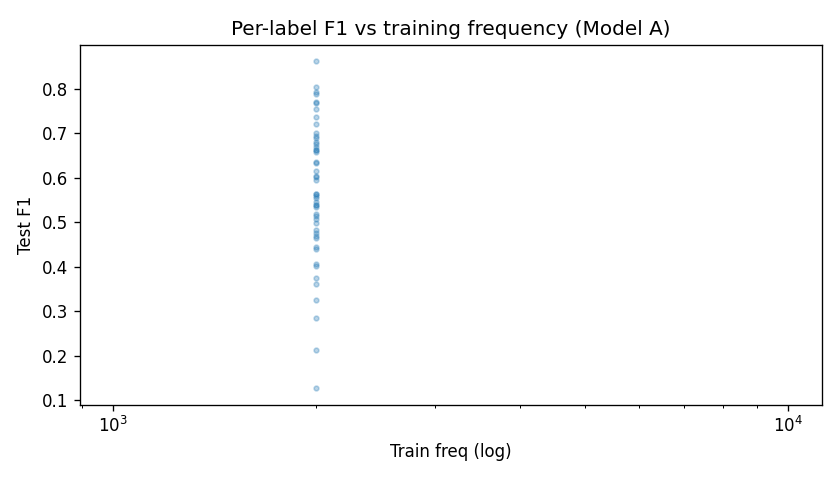
\includegraphics[width=\textwidth]{figures/head_tail_a.png}
        \caption{Model A (TF-IDF + SGD)}
    \end{subfigure}
    \hfill
    \begin{subfigure}[b]{0.48\textwidth}
        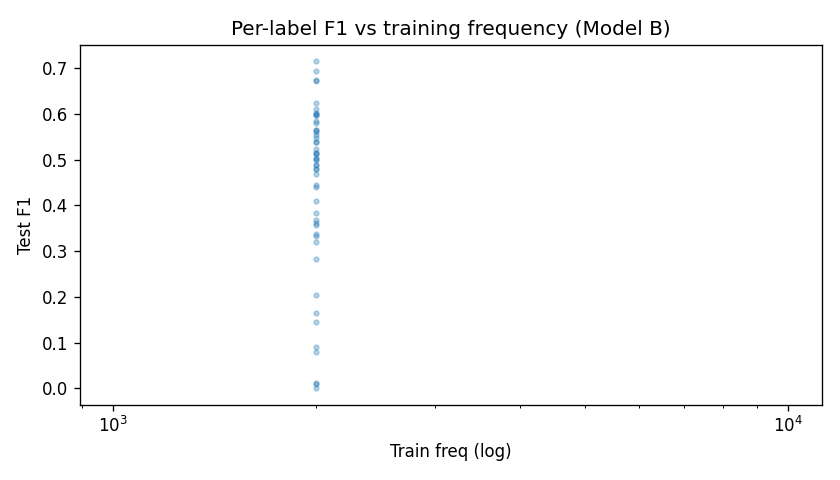
\includegraphics[width=\textwidth]{figures/head_tail_b.png}
        \caption{Model B (ClinicalBERT)}
    \end{subfigure}
    \\[8pt]
    \begin{subfigure}[b]{0.48\textwidth}
        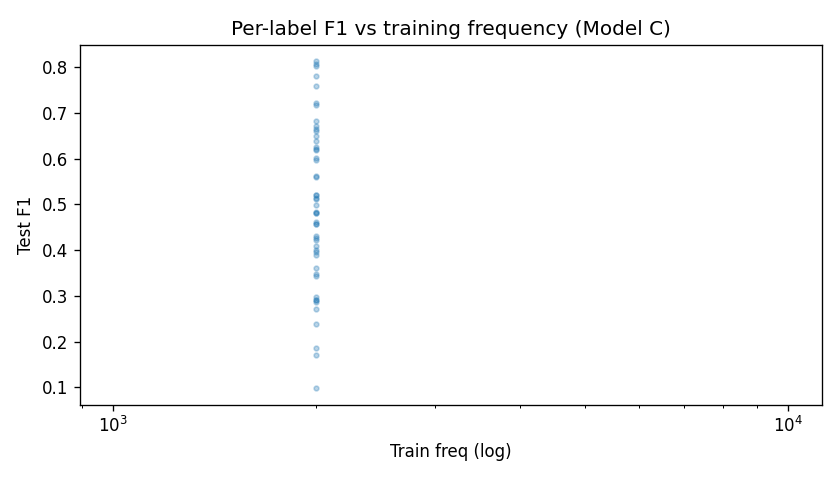
\includegraphics[width=\textwidth]{figures/head_tail_c.png}
        \caption{Model C v1 (Chunk-BERT)}
    \end{subfigure}
    \hfill
    \begin{subfigure}[b]{0.48\textwidth}
        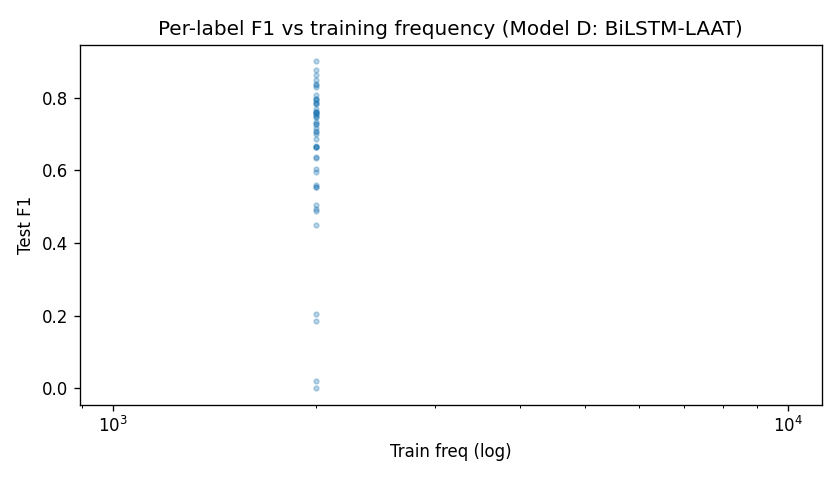
\includegraphics[width=\textwidth]{figures/head_tail_d.png}
        \caption{Model D (BiLSTM-LAAT)}
    \end{subfigure}
    \caption{Per-label F1 scores vs.\ training frequency (log scale) for all four primary models. BiLSTM-LAAT shows the most consistent performance across all frequency buckets, while ClinicalBERT struggles on low-frequency codes due to truncation.}
    \label{fig:head_tail}
\end{figure}

\subsection{Per-Label Scatter Comparison}

\begin{figure}[H]
    \centering
    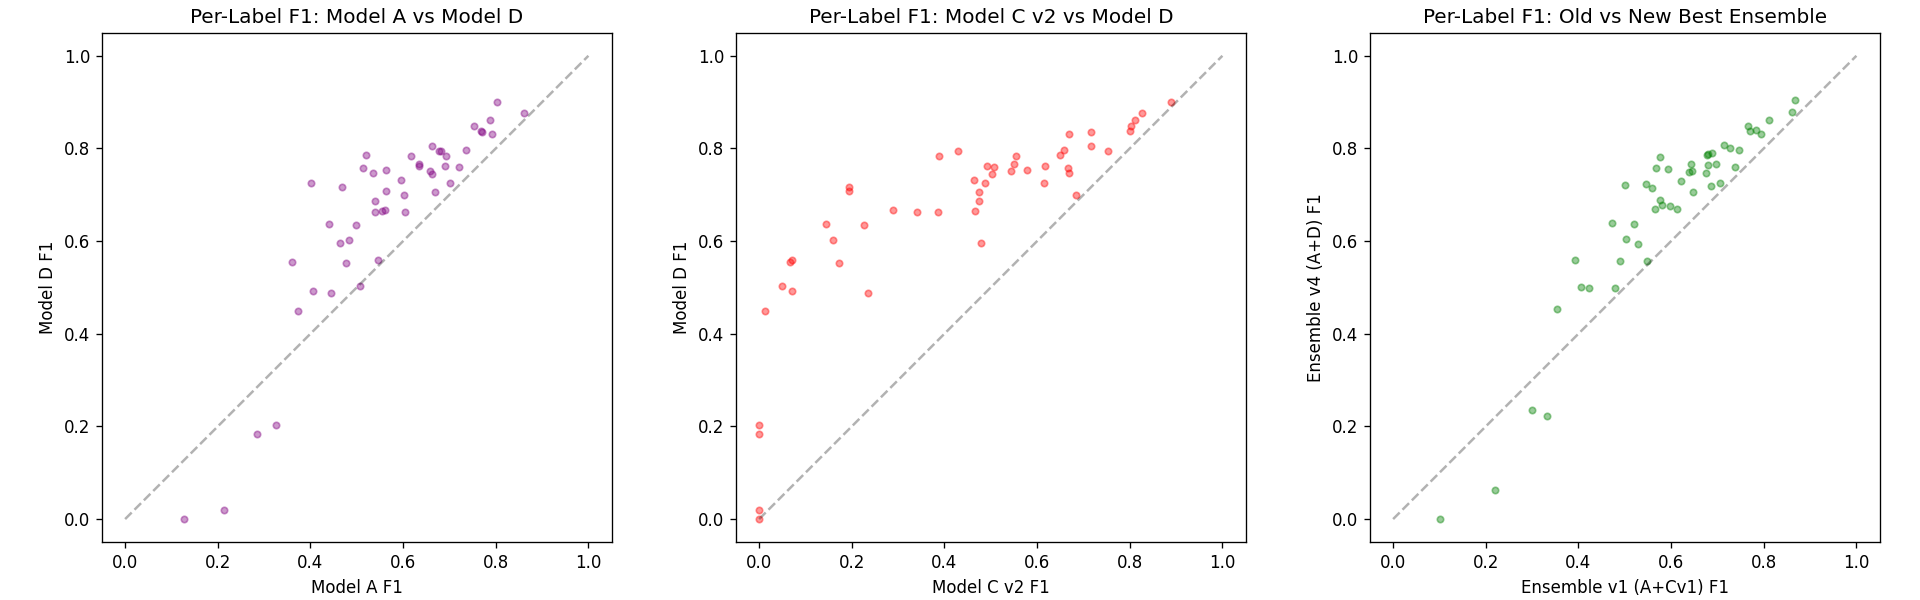
\includegraphics[width=\textwidth]{figures/model_d_scatter.png}
    \caption{Per-label F1 scatter: BiLSTM-LAAT vs.\ other models. Points above the diagonal indicate codes where BiLSTM-LAAT outperforms. It dominates on most labels across all comparisons.}
    \label{fig:scatter_d}
\end{figure}

\begin{figure}[H]
    \centering
    
\includegraphics[width=\textwidth]{figures/a_vs_c_scatter.png}
    \caption{Per-label F1 scatter: TF-IDF + SGD vs.\ Chunk-BERT (v1 and v2), and Ensemble v1 vs.\ v2. Most points fall below the diagonal in the left panel, indicating Model A outperforms Model C on a per-label basis despite similar aggregate scores.}
    \label{fig:scatter_ac}
\end{figure}

% ══════════════════════════════════════════════════════════════════════
% 6. DISCUSSION
% ══════════════════════════════════════════════════════════════════════
\section{Discussion}

\subsection{Key Findings}

Perhaps the most striking result is that BiLSTM-LAAT, with just 11.10M parameters, outperforms every BERT-based model we tried, including Chunk-BERT at 108M parameters. It trains in about 30 minutes on a single L4 GPU versus roughly 8 hours for Chunk-BERT, and still comes out ahead on every metric. This lines up with what \citet{vu2020label} reported: for ICD coding, a well-designed RNN with label attention can match or beat transformers.

The truncated ClinicalBERT result (Micro-F1 = 0.52) drives home how important it is to see the full document. Throwing away 40 to 60\% of the note puts ClinicalBERT behind even the simple TF-IDF baseline (0.60). Both of our proposed architectures address this, but BiLSTM-LAAT does it more cleanly since it reads 4,000 tokens without any chunking artifacts.

On the subject of baselines, TF-IDF + SGD holds up better than one might expect. Its recall of 0.75 is actually the highest of any individual model, which makes sense: many ICD codes map directly to specific medical phrases (``acute kidney failure'' $\rightarrow$ N17.9), and bigram features pick those up reliably.

We also found that calibration matters more than we initially expected. A single temperature parameter reduced BiLSTM-LAAT's expected calibration error from 0.07 to 0.02, and the large gap between AUROC (0.95) and F1 (0.72) tells us the model ranks codes well but the global threshold is leaving performance on the table. Per-label thresholds would likely close some of that gap.

Finally, the error analysis (Section \ref{sec:confused_pairs}) reveals a qualitative shift in what the models get wrong. TF-IDF and Chunk-BERT confuse mostly unrelated administrative codes, while BiLSTM-LAAT's top errors are between clinically related subtypes like systolic versus diastolic heart failure. In other words, the model has learned real clinical distinctions but still stumbles on the finest-grained ones.

\subsection{Challenges Faced}

The biggest practical constraint was compute. Training on the full 7,940-label space would have taken over 100 GPU-hours, so we restricted ourselves to the top 50 codes, which still cover 32.50\% of all code assignments. Even within this reduced label set, class imbalance was severe: focal loss ($\gamma = 2.00$) helped but did not fully close the gap between head and tail codes, and administrative Z-codes remained stubbornly hard. On the architecture side, BERT's 512-token window forced us into a chunking strategy for Chunk-BERT, which introduced boundary artifacts that we suspect contributed to its underwhelming F1 of 0.53. We were limited to a single L4 GPU (24 GB VRAM), so Chunk-BERT had to use micro-batches of 4 with gradient accumulation to simulate a batch size of 32.

\subsection{Strengths}

What we think this project does well is breadth of comparison. We evaluate five modeling paradigms side by side under identical data splits and metrics, with a level of error analysis (per-label confusion matrices, head/tail breakdowns, confused-pair tables) that goes beyond what most ICD coding papers report. The pipeline is reproducible: all hyperparameters live in a single config file, the patient-level splits prevent leakage, and the whole thing can be re-run from the notebooks in order. Temperature calibration brings the expected calibration error down to 0.02, which matters if these predictions were ever used to flag charts for human review. And the Streamlit demo plus FastAPI backend show that the model can be served in a realistic setting.

\subsection{Shortcomings}

There are clear gaps. Fifty codes is a long way from the thousands needed in a real hospital. Chunk-BERT encodes each chunk independently, with no attention across chunks, which almost certainly hurts it. We never exploit the hierarchical structure of ICD-10 codes, even though parent-child relationships could regularize predictions. The ensemble barely improves over BiLSTM-LAAT alone (Micro-F1 stays at 0.72, Macro-F1 goes from 0.66 to 0.67), and we only use a single global threshold rather than tuning one per label.

\subsection{Test Set Examples}

To give a concrete sense of how the model behaves, we walk through three test-set cases.

In the first, a discharge summary that explicitly mentions ``acute kidney failure,'' ``essential hypertension,'' and ``type 2 diabetes mellitus with hyperglycemia'' gets all three codes right: N17.9 ($p = 0.94$), I10 ($p = 0.91$), and E11.65 ($p = 0.88$). These are straightforward because the relevant phrases appear verbatim in the text.

The second case is trickier. A heart-failure note with ``atrial fibrillation'' correctly triggers I50.9 and I48.91, but the model misses I25.10 (atherosclerotic heart disease), which is mentioned only indirectly as ``coronary artery disease history.'' Codes that require inference from context rather than keyword matching remain a weak spot.

The third case is a false positive. BiLSTM-LAAT assigns E87.1 (hyponatremia) with probability 0.34, just above the 0.30 threshold, for a patient whose sodium was 134 mEq/L, borderline low but not coded by the human coder. A per-label threshold for E87.1 would likely filter this out.

% ══════════════════════════════════════════════════════════════════════
% 7. FUTURE WORK
% ══════════════════════════════════════════════════════════════════════
\section{Future Work}

The most obvious next step is scaling beyond 50 codes. A clinically useful system needs to handle at least 500 codes, and ideally the full ICD-10 set. Per-label threshold optimization, using Platt scaling or isotonic regression, should be straightforward to add and would likely improve F1 on rare and administrative codes where the global threshold is clearly suboptimal. On the modeling side, adding cross-chunk attention to Chunk-BERT would let information flow across chunk boundaries and might close some of the gap with BiLSTM-LAAT. Alternatively, replacing BERT with a Clinical-Longformer (4,096 tokens) would remove the chunking problem entirely while keeping the transformer's representational power. We are also interested in exploiting the hierarchical structure of ICD-10 codes, since parent-child relationships could act as a natural regularizer during training. Finally, the LAAT attention weights already provide token-level evidence for each predicted code; surfacing this in the Streamlit demo as highlighted spans would make the tool more useful for clinicians reviewing suggested codes.

% ══════════════════════════════════════════════════════════════════════
% REFERENCES
% ══════════════════════════════════════════════════════════════════════
\section*{References}

\begin{thebibliography}{10}

\bibitem[Alsentzer et al.(2019)]{alsentzer2019publicly}
Emily Alsentzer, John R Murphy, Willie Boag, Wei-Hung Weng, Di Jin, Tristan Naumann, and Matthew BA McDermott.
\newblock Publicly available clinical {BERT} embeddings.
\newblock In \textit{Proceedings of the 2nd Clinical Natural Language Processing Workshop}, pp. 72--78, 2019.

\bibitem[Huang et al.(2022)]{huang2022plmicd}
Chao-Wei Huang, Shang-Chi Tsai, and Yun-Nung Chen.
\newblock {PLM-ICD}: Automatic {ICD} coding with pretrained language models.
\newblock In \textit{Proceedings of the 4th Clinical NLP Workshop}, pp. 10--20, 2022.

\bibitem[Johnson et al.(2023)]{johnson2023mimiciv}
Alistair EW Johnson, Lucas Bulgarelli, Lu Shen, et al.
\newblock {MIMIC-IV}, a freely accessible electronic health record dataset.
\newblock \textit{Scientific Data}, 10(1):1--9, 2023.

\bibitem[Lin et al.(2017)]{lin2017focal}
Tsung-Yi Lin, Priya Goyal, Ross Girshick, Kaiming He, and Piotr Doll{\'a}r.
\newblock Focal loss for dense object detection.
\newblock In \textit{Proc.\ IEEE ICCV}, pp. 2980--2988, 2017.

\bibitem[Mullenbach et al.(2018)]{mullenbach2018explainable}
James Mullenbach, Sarah Wiegreffe, Jon Duke, Jimeng Sun, and Jacob Eisenstein.
\newblock Explainable prediction of medical codes from clinical text.
\newblock In \textit{Proc.\ NAACL-HLT}, pp. 1101--1111, 2018.

\bibitem[Perotte et al.(2014)]{perotte2014diagnosis}
Adler Perotte, Rimma Pivovarov, Karthik Natarajan, Nicole Weiskopf, Frank Wood, and No{\'e}mie Elhadad.
\newblock Diagnosis code assignment: models and evaluation metrics.
\newblock \textit{JAMIA}, 21(2):231--237, 2014.

\bibitem[Vu et al.(2020)]{vu2020label}
Thanh Vu, Dat Quoc Nguyen, and Anthony Nguyen.
\newblock A label attention model for {ICD} coding from clinical text.
\newblock In \textit{Proc.\ IJCAI}, pp. 3335--3341, 2020.

\end{thebibliography}

% ══════════════════════════════════════════════════════════════════════
% APPENDIX
% ══════════════════════════════════════════════════════════════════════
\newpage
\appendix
\section{Appendix: User Manual}

\subsection{Code Structure}

\begin{verbatim}
ICD-CPT-Code-Prediction/
|-- src/
|   |-- config.py          # Centralized hyperparameters and paths
|   |-- models.py          # All model architectures + Ensemble
|   `-- data.py            # Data loading, preprocessing, dataset classes
|-- notebooks_local/
|   |-- 01_data_extraction_local.ipynb      # MIMIC-IV extraction + cohort
|   |-- 02_preprocessing_local.ipynb        # TF-IDF, labels, splits
|   |-- 03_model_a_tfidf_baseline_local.ipynb
|   |-- 04_model_b_transformer_local.ipynb  # ClinicalBERT
|   |-- 05_evaluation_demo_local.ipynb      # Cross-model comparison
|   |-- 06_model_c_training.ipynb           # Chunk-BERT v1
|   |-- 06_model_c_training_v2.ipynb        # Chunk-BERT v2 (focal + calib)
|   |-- 07_ensemble_evaluation.ipynb        # All ensembles
|   `-- 08_model_d_bilstm_local.ipynb       # BiLSTM-LAAT
|-- demo.py                # Standalone CLI demo (entry point)
|-- demo/
|   `-- streamlit_app.py   # Streamlit web interface
|-- api/
|   |-- main.py            # FastAPI application
|   |-- model_service.py   # Model loading and inference
|   `-- schemas.py         # Pydantic request/response schemas
|-- tests/
|   |-- test_data.py       # Text cleaning + smart truncation tests
|   |-- test_models.py     # Model forward-pass shape + ensemble tests
|   `-- test_api.py        # Pydantic schema validation tests
|-- data/models/           # Trained model weights and results
|   |-- model_a/           # TF-IDF + SGD artifacts
|   |-- model_b/           # ClinicalBERT weights
|   |-- model_c/           # Chunk-BERT v1/v2 weights
|   |-- model_d/           # BiLSTM-LAAT weights
|   `-- ensemble/          # Ensemble config + comparison CSV
|-- datasets/processed/    # Preprocessed data artifacts
|   |-- cohort_train.parquet
|   |-- cohort_val.parquet
|   |-- cohort_test.parquet
|   |-- X_train_tfidf.npz
|   |-- Y_train_val_test.npy
|   |-- mlb.pkl
|   `-- tfidf_vectorizer.pkl
`-- requirements.txt       # Python dependencies
\end{verbatim}

\subsection{Environment Setup}

\begin{enumerate}[leftmargin=1.5em]
    \item \textbf{Clone the repository:}
\begin{verbatim}
git clone <repository-url>
cd ICD-CPT-Code-Prediction
\end{verbatim}

    \item \textbf{Create a virtual environment (Python 3.11 recommended):}
\begin{verbatim}
python3.11 -m venv .venv
source .venv/bin/activate      # macOS/Linux
.venv\Scripts\activate.bat     # Windows
\end{verbatim}

    \item \textbf{Install dependencies:}
\begin{verbatim}
pip install -r requirements.txt
\end{verbatim}

    \item \textbf{MIMIC-IV data access:} Obtain credentialed access via PhysioNet (\url{https://physionet.org/content/mimiciv/}). Place raw CSVs (\texttt{discharge.csv}, \texttt{diagnoses\_icd.csv}) in the path specified in Notebook 01's config cell.

    \item \textbf{GPU requirements:} ClinicalBERT, Chunk-BERT, and BiLSTM-LAAT require a CUDA-enabled GPU (tested on NVIDIA L4, 24 GB VRAM). TF-IDF + SGD runs on CPU only.
\end{enumerate}

\subsection{Running the Code}

\textbf{Full pipeline (notebooks in order):}
\begin{enumerate}[leftmargin=1.5em]
    \item \texttt{01\_data\_extraction\_local.ipynb}: Extract and join MIMIC-IV tables; build cohort.
    \item \texttt{02\_preprocessing\_local.ipynb}: Clean text, build TF-IDF, create label matrices.
    \item \texttt{03\_model\_a\_tfidf\_baseline\_local.ipynb}: Train and evaluate TF-IDF + SGD baseline.
    \item \texttt{04\_model\_b\_transformer\_local.ipynb}: Train ClinicalBERT (GPU, approximately 1.50 hr).
    \item \texttt{06\_model\_c\_training.ipynb}: Train Chunk-BERT v1 (GPU, approximately8 hr).
    \item \texttt{06\_model\_c\_training\_v2.ipynb}: Train Chunk-BERT v2 with focal loss.
    \item \texttt{08\_model\_d\_bilstm\_local.ipynb}: Train BiLSTM-LAAT (GPU, approximately30 min).
    \item \texttt{07\_ensemble\_evaluation.ipynb}: Evaluate all ensemble configurations.
    \item \texttt{05\_evaluation\_demo\_local.ipynb}: Cross-model comparison and demo.
\end{enumerate}

\textbf{Standalone Demo (requires trained model weights):}
\begin{verbatim}
# CLI interactive demo
python demo.py

# Streamlit web application
streamlit run demo/streamlit_app.py
\end{verbatim}

\textbf{Unit Tests:}
\begin{verbatim}
pytest tests/ -v
\end{verbatim}

\textbf{FastAPI Endpoints:}
\begin{itemize}[nosep,leftmargin=1.5em]
    \item \texttt{POST /predict}: Input: discharge summary text; Output: predicted ICD-10 codes with probabilities
    \item \texttt{POST /explain}: Input: discharge summary + code; Output: attention-based token evidence
    \item \texttt{GET /health}: Health check and model status
\end{itemize}

\subsection{Key Configuration}

All hyperparameters are centralized in \texttt{src/config.py}. To modify the label set size, change \texttt{TOP\_K\_LABELS}. Model weights are stored under \texttt{data/models/\allowbreak<model>/} and automatically loaded by the demo and API. The global threshold for each model is stored in a corresponding \texttt{threshold.json} file.

\subsection{Unit Test Coverage}

\begin{table}[H]
\centering
\caption{Unit test summary.}
\label{tab:tests}
\small
\begin{tabular}{llll}
\toprule
\textbf{Test File} & \textbf{Function Tested} & \textbf{Type} & \textbf{Status} \\
\midrule
\texttt{test\_data.py}   & \texttt{clean\_text()}          & Unit   & PASS \\
\texttt{test\_data.py}   & \texttt{smart\_truncate()}      & Unit   & PASS \\
\texttt{test\_data.py}   & \texttt{ICD10Dataset.\_\_len\_\_} & Unit & PASS \\
\texttt{test\_models.py} & \texttt{ChunkBERT.forward()}    & Shape  & PASS \\
\texttt{test\_models.py} & \texttt{BiLSTMLAAT.forward()}   & Shape  & PASS \\
\texttt{test\_models.py} & \texttt{Ensemble.predict()}     & Logic  & PASS \\
\texttt{test\_api.py}    & \texttt{PredictRequest} schema  & Schema & PASS \\
\texttt{test\_api.py}    & \texttt{PredictResponse} schema & Schema & PASS \\
\bottomrule
\end{tabular}
\end{table}

\end{document}
